\chapter{Mạng và mạng Internet}

\minitoc
\vspace{0.5cm}
\noindent
Trong chương này, ta sẽ thảo luận xung quanh khái niệm mạng; bao gồm việc nghiên cứu xem các máy tính kết nối với nhau, chia sẻ thông tin và
tài nguyên như thế nào. Ta cũng xem xét các  cấu trúc và điều khiển của hệ thống mạng, các ứng dụng mạng và những vấn đề liên quan đến an ninh
mạng. Chủ đề nổi bật trong chương này là mạng Internet, hệ thống kết nối các hệ thống mạng trên phạm vi toàn cầu.

%Nhu cầu chia sẻ thông tin và tài nguyên giữa các máy tính khác nhau dẫn tới các hệ thống
%máy tính được kết nối, gọi là các \textbf{mạng máy tính}, trong đó các máy tính được kết
%nối để dữ liệu có thể được truyền từ máy này sang máy khác. Trong các mạng máy tính này,
%người sử dụng có thể trao đổi các thông điệp và tài nguyên chia sẻ nằm rải rác trong toàn bộ hệ thống--như máy in, các gói
%phần mềm, và các phương tiện lưu trữ dữ liệu. Những
%phần mềm cơ bản đòi hỏi hỗ trợ như các ứng dụng từ những gói công cụ đơn giản cho đến một
%hệ thống mở rộng của phần mềm mạng mà cung cấp một cơ sở hạ tầng rộng lớn cho hệ thống
%mạng phức tạp. Theo một nghĩa nào đó, phần mềm mạng đang tiến hóa thành một hệ điều hành mạng lớn. %Trong
%chương này ta sẽ nghiên cứu lĩnh vực mở rộng này của khoa học máy tính.
%-----------------

 
   
\section{Cơ bản về mạng}
\label{sec:4.1}
Ta bắt đầu với các khái niệm cơ bản về mạng.

\subsection*{Phân loại hệ thống mạng}

Một mạng máy tính thường được phân loại dựa trên đặc tính về khoảng cách địa lý như
\textbf{mạng cục bộ (LAN)}, \textbf{mạng đô thị (MAN)} hay \textbf{mạng diện rộng
  (WAN)}. Mạng LAN thường bao gồm một tập hợp các máy tính trong một tòa nhà đơn lẻ hay
một liên hợp các tòa nhà. Ví dụ, các máy tính trong một khuôn viên trường đại học hay
trong một nhà máy chế tạo máy móc có thể được kết nối với nhau thông qua mạng LAN.  Mạng
MAN là mạng có phạm vi trung bình, ví dụ như mạng mở rộng trong phạm vi một địa phương cục
bộ.  Mạng WAN nối kết các thiết bị mạng có tầm khoảng cách lớn hơn, ví dụ như khoảng cách
giữa các thành phố hay giữa các vị trí trên thế giới.

Một cách thức phân loại mạng khác là chia thành mạng thành hai loại: \textbf{mạng mở} và
\textbf{mạng đóng}. Mạng mở là mạng mà sự vận hành bên trong của nó được dựa trên những
thiết kế trong một phạm vi công cộng. Mạng đóng là mạng được thiết kế của nó dựa trên
chính sự đổi mới của nó và được điều khiển bởi một cá nhân hay một tổ chức nào đó.

Một ví dụ về mạng mở là mạng Internet (mạng phạm vi toàn cầu). Trong mạng Internet, việc truyền thông tin được điều khiển bởi một tập các quy tắc chuẩn mở được thừa nhận rộng rãi như bộ giao thức TCP/IP. Mọi người đều có thể sử dụng những quy tắc chuẩn này mà
không phải trả phí cũng như không phải ký kết một thỏa thuận nào về quyền sử dụng. Ngược lại, các công ty như Novell, thường phát triển  hệ thống và duy trì quyền sở hữu của họ. Điều này cho phép công ty có thể thu được lợi nhuận từ việc bán
hay cho thuê các sản phẩm này. Những mạng dựa trên những hệ thống như vậy là ví dụ
về các mạng đóng.

\begin{figure}[tbh] 
\centering
    \scalebox{0.45}{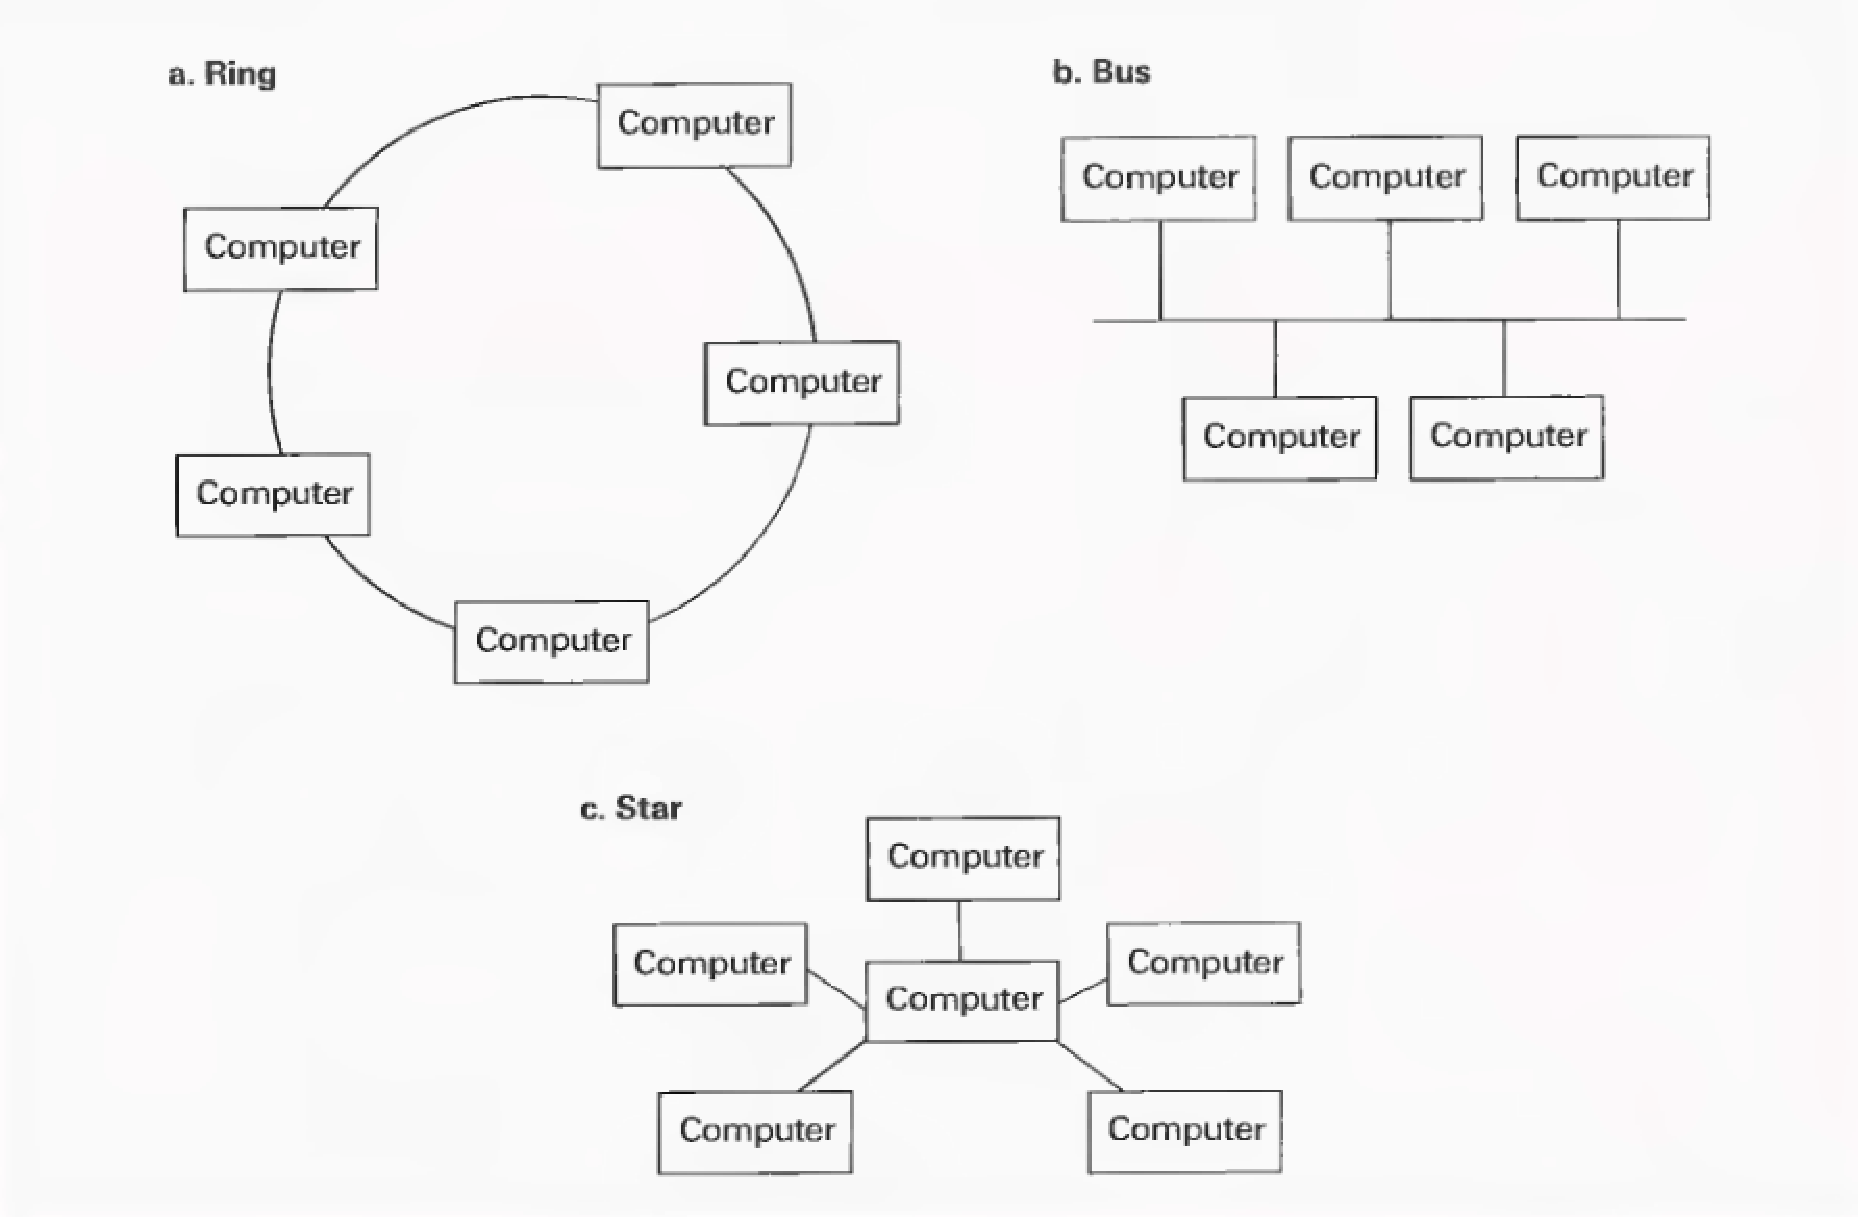
\includegraphics{ch5/fig41.pdf}}
\caption{Các hình trạng mạng}
  \label{fig:fig4.1}
\end{figure}

Còn một cách phân loại mạng khác đó là dựa trên hình trạng của mạng. Hình trạng mạng
là mô hình xác định cách để các thiết bị trong mạng kết nối với nhau. Hình~\ref{fig:fig4.1} giới
thiệu ba hình trạng mạng phổ biến:
\begin{inparaenum}[(1)]
\item Mạng vòng tròn (Ring), trong đó các thiết bị được kết nối với nhau
  theo hình tròn;
\item Mạng hình tuyến (Bus), trong đó tất cả các thiết bị được kết nối với nhau thông qua
  một đường truyền tải gọi là trục chính (Bus); và
\item Mạng hình sao, trong đó một thiết bị phục vụ như là một điểm trung tâm nơi mà các
  thiết bị khác được kết nối tới nó.
\end{inparaenum}

Trong những mô hình trên, mạng hình sao được sử dụng phổ biến nhất. Mạng này đã
phát triển từ mô hình trung tâm máy tính lớn phục vụ cho nhiều người sử dụng. Thể hiện rõ nhất là trường hợp những người dùng sử dụng các thiết bị đầu cuối kết nối vào các máy tính nhỏ. Ngày nay, mô hình mạng hình tuyến (bus) cũng
được sử dụng rộng rãi dưới hình thức mạng chuẩn là \textbf{Ethernet}, một
trong những mô hình mạng khá phổ biến.

Cần chú ý rằng hình trạng của mạng có thể không  thể hiện rõ qua mô hình vật
lý của nó. Ví dụ, một mạng hình tuyến (bus) không nhất thiết phải được triển khai
dưới một đường trục dài nơi mà các máy tính được kết nối thông qua các liên kết ngắn như
đã mô tả trong Hình~\ref{fig:fig4.1}. Thay vào đó, thông thường người ta dựng một mạng
hình tuyến bằng cách chạy các liên kết từ chính mỗi máy tính tới một vùng trung tâm, nơi
mà chúng được kết nối với nhau thông qua một thiết bị gọi là \textbf{hub}. Thiết bị hub
này nhỏ hơn bất kỳ một trục ngắn nào. Nó thực hiện tiếp sóng bất kỳ tín hiệu nào nó nhận
được (thông qua một vài bộ khuếch đại tín hiệu) và truyền tới tất cả các máy tính kết nối
với nó thông qua các cổng. Kết quả là một mạng trông như mạng hình sao lại được hoạt động
dưới hình thức là một mạng hình tuyến. Sự khác nhau ở đây là thiết bị trung tâm trong mô
hình mạng hình sao là một máy tính (thường là một thiết bị với nhiều khả năng hơn tại các
điểm nút của hình sao); nó  nhận và xử lý các thông điệp từ các máy tính khác. Ngược lại, thiết
bị trung tâm trong mô hình mạng hình tuyến là một hub; nó  chỉ đơn thuần cung cấp một kênh truyền
thông tin cho các máy tính.

Một quan điểm khác cũng cần phải chú ý là các kết nối giữa các thiết bị trong hệ thống
mạng không nhất thiết phải là các thiết bị vật lý. Hệ thống mạng không dây, sử dụng công
nghệ truyền phát qua sóng radio, cũng dần được sử dụng phổ biến. Đặc biệt, thiết bị hub
trong rất nhiều mô hình mạng hình tuyến ngày nay thực chất là một trạm tiếp và phát sóng
radio.

\subsection*{Các giao thức}
Để cho một hệ thống mạng hoạt động tin cậy, việc thiết lập những quy tắc nhờ
đó các hoạt động của mạng được kiểm soát là rất quan trọng. Những quy tắc này được gọi là
các \textbf{giao thức}. Thông qua việc phát triển và kế thừa các chuẩn giao thức, các nhà
cung cấp có thể xây dựng những sản phẩm cho các ứng dụng mạng tương thích với những sản
phẩm của nhà cung cấp khác. Việc phát triển các chuẩn giao thức là quá trình không
thể thiếu trong sự phát triển các công nghệ mạng.


Khi giới thiệu về khái niệm giao thức, ta hãy xem xét vấn đề  phối hợp truyền thông điệp giữa các máy tính trong một mạng. Nếu không có các quy tắc  quản lý quá
trình truyền  này, các máy tính có thể yêu cầu truyền thông điệp vào cùng một
thời điểm hoặc cũng có thể bị lỗi khi tiếp nhận các thông điệp khi hỗ trợ đó được yêu cầu.


\begin{figure}[tbh] 
\centering
    \scalebox{0.45}{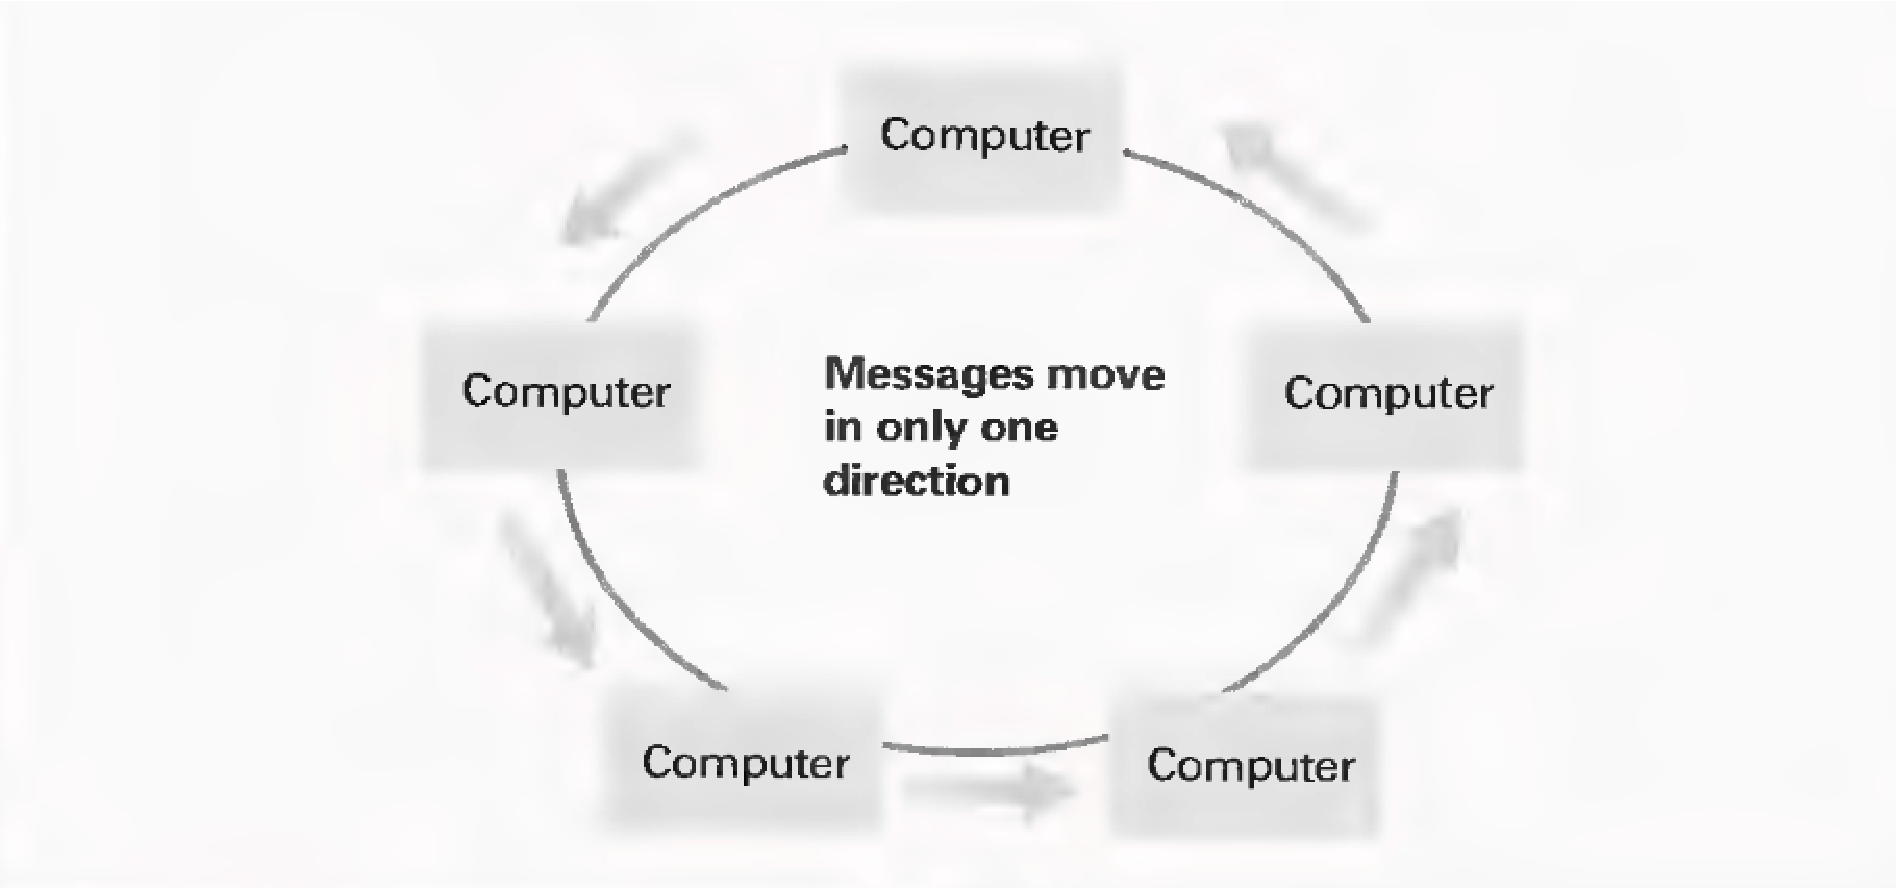
\includegraphics{ch5/fig42.pdf}}
    \caption{Truyền thông trong mạng vòng tròn}
  \label{fig:fig4.2}
\end{figure}

Một cách tiếp cận để có thể giải quyết được vấn đề này là giao thức \textbf{thẻ bài} trong
mạng vòng, được phát triển bởi IBM từ  những năm 1970 và tiếp tục trở nên phổ biến
trong các hệ thống mạng dựa trên nền tảng mô hình mạng vòng. Với giao thức này, tất
cả các thiết bị trong mạng truyền tải thông điệp theo một hướng chung duy nhất
(Hình~\ref{fig:fig4.2}), nghĩa là tất cả các thông điệp đó được gửi qua mạng di chuyển
vòng tròn theo cùng một hướng bằng cách chuyển tiếp từ máy tính này tới máy tính khác. Khi
một thông điệp được truyền tới đích của nó, máy tính đích giữ lại một bản sao và chuyển
tiếp một bản sao của thông điệp đó sang máy tính tiếp theo theo hình tròn. Khi bản sao
được chuyển tiếp về tới máy tính ban đầu, máy tính đó nhận thấy rằng thông điệp này đã
truyền được tới đích cần thiết, nó sẽ loại bỏ thông điệp ra khỏi vòng tròn. Tất nhiên, hệ
thống này còn phụ thuộc vào sự hợp tác của các liên máy tính. Nếu một máy tính yêu cầu
truyền phát liên tục các thông điệp từ chính nó thay vì chuyển tiếp các thông điệp sang
máy tính khác thì không có quá trình truyền tải nào được hoàn thành.


Để giải quyết vấn đề này, một xâu bít duy nhất, gọi là thẻ bài, được sử dụng trong quá
trình truyền tải theo vòng tròn. Quyền sở hữu của thẻ bài này được trao cho máy tính
nguồn, nơi bắt đầu truyền phát thông điệp; nếu không có thẻ bài, một máy tính chỉ được
phép chuyển tiếp thông điệp mà nó nhận được. Thông thường, mỗi máy tính đơn thuần chỉ tiếp
nhận và chuyển tiếp thẻ bài theo đúng cách mà nó chuyển tiếp thông điệp. Tuy nhiên, nếu
máy tính nhận được thẻ bài có thông điệp của chính nó đưa lên mạng, nó sẽ truyền một thông
điệp trong khi giữ lại thẻ bài. Khi thông điệp này hoàn tất quá trình truyền tải qua một
vòng tròn, máy tính chuyển tiếp thẻ bài cho máy tính tiếp theo trong vòng tròn. Như vậy,
khi máy tính tiếp theo nhận được thẻ bài, nó có thể chuyển tiếp thẻ bài ngay lập tức hoặc
truyền phát một thông điệp mới của mình trước khi chuyển tiếp thẻ bài cho máy tính tiếp
theo. Theo cách thức này, mỗi máy tính trong mạng đều có cơ hội như nhau để có thể gửi
thông điệp của nó cũng như thẻ bài đi xung quanh vòng tròn.


\begin{figure}[tbh]
\centering
    \scalebox{0.4}{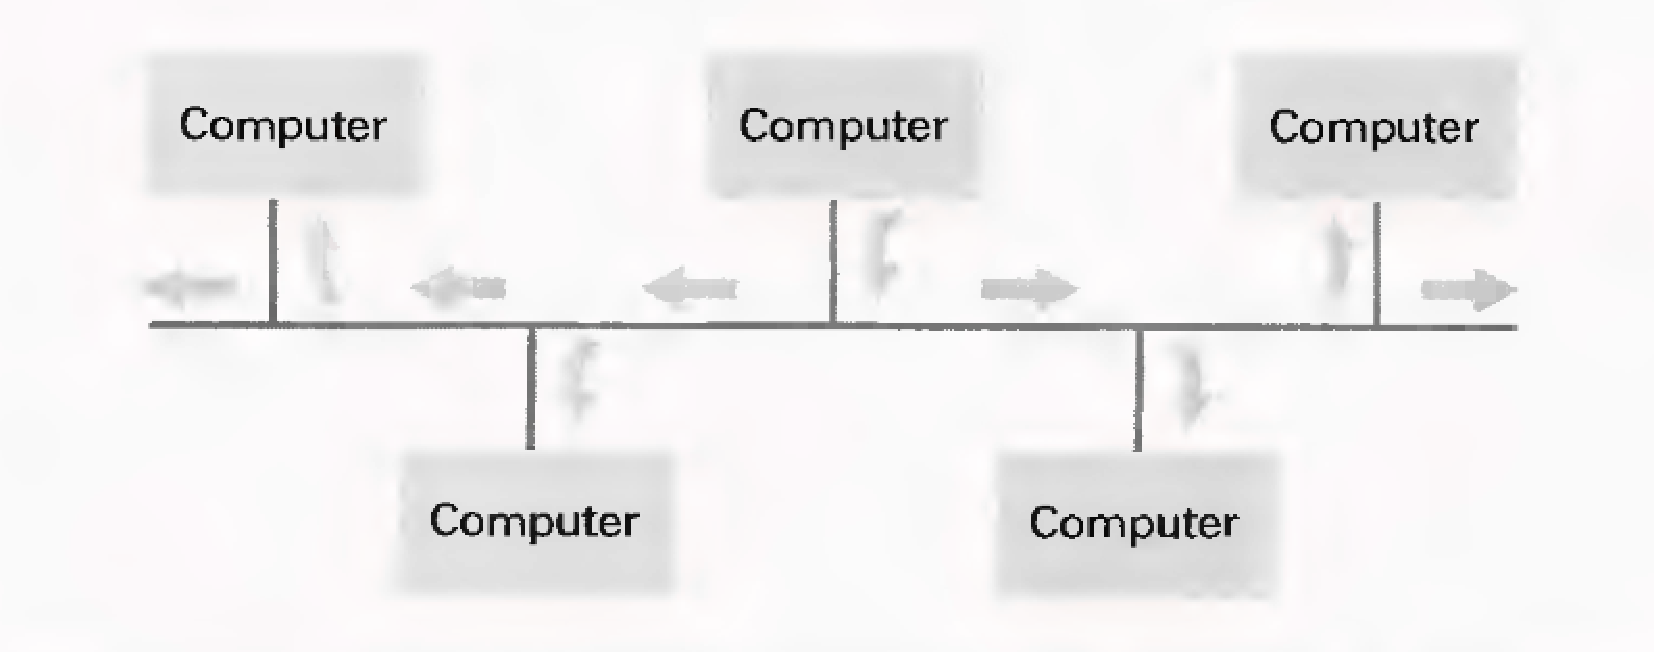
\includegraphics{ch5/fig43.pdf}}
    \caption{Truyền thông trong mạng hình tuyến}
  \label{fig:fig4.3}
\end{figure}

Một giao thức khác cũng được sử dụng trong công nghệ mạng hình tuyến cho việc phối hợp
truyền tải các thông điệp, đó là giao thức dựa trên tập các giao thức Ethernet. Trong hệ
thống mạng Ethernet, quyền truyền tải thông điệp được điều khiển bởi giao thức \textbf{Đa
  truy nhập có thăm dò và tách đụng độ} (Carrier Sense, Multiple Access with Collision
Detection--CSMA/CD). Giao thức này yêu cầu mỗi thông điệp phải được quảng bá cho tất cả
các máy tính trong trục chính (Hình~\ref{fig:fig4.3}). Mỗi máy tính sẽ theo dõi tất cả các
thông điệp những chỉ giữ lại những thông điệp nào được gửi tới chính nó thông qua địa
chỉ. Để truyền phát một thông điệp, một máy tính đợi cho đến khi đường trục chính rỗi, và
tại thời điểm này nó sẽ bắt đầu truyền phát tín hiệu trong khi tiếp tục theo dõi đường
trục chính. Nếu một máy tính khác cũng bắt đầu truyền tín hiệu, cả hai máy tính sẽ phát
hiện ra sự xung đột và sẽ tạm dừng trong một khoảng thời gian ngẫu nhiên trước khi truyền
tín hiệu lại. Một nhóm nhỏ người có nhu cầu đàm luận với nhau có thể sử dụng một hệ thống
tương đương như vậy. Nếu hai người cùng bắt đầu nói tại một thời điểm, cả hai sẽ dừng
lại. Một trong hai người có thể sẽ tiếp tục với một chuỗi câu như ``Xin lỗi, anh định nói
gì vậy?'', ``Không, không. Anh nói trước đi'', trong khi với giao thức CSMA/CD, mỗi máy
tính đơn thuần chỉ là thử truyền phát tín hiệu lại.


\subsection*{Kết hợp các hệ thống mạng}

Đôi khi cần phải kết nối các hệ thống mạng đã tồn tại thành một hệ thống truyền thông mở
rộng. Điều này có thể được thực hiện bằng việc kết nối các mạng thành một phiên bản lớn
hơn nhưng vẫn cùng ``kiểu'' như hệ thống cũ. Ví dụ, trong trường hợp những hệ thống mạng
hình tuyến dựa trên các giao thức mạng Ethernet, thông thường có thể kết nối các trục
chính thành một trục đơn lớn hơn. Việc này được thực hiện với điều kiện sử dụng các thiết
bị khác nhau được biết đến như\textbf{ bộ lặp tín hiệu} (repeater), \textbf{cầu nối}
(bridge), và \textbf{bộ chuyển mạch} (switch), đó là những sự khác biệt không dễ phát hiện
ra nhằm phục vụ cho việc mở rộng hệ thống mạng. Đơn giản nhất trong số đó là bộ lặp tín
hiệu, thiết bị dùng để kết nối trục chính của hai mạng hình tuyến lại với nhau thành một
trục dài hơn (Hình~\ref{fig:fig4.4}). Bộ khuếch đại (bộ lặp tín hiệu) đơn giản chỉ truyền
các tín hiệu về phía sau hay trước giữa hai tuyến gốc ban đầu (thông thường sử dụng với
một vài bộ khuếch đại tín hiệu) mà không cần biết ý nghĩa của những tín hiệu đó là gì.

\begin{figure}[tb] 
  \centering \scalebox{0.45}{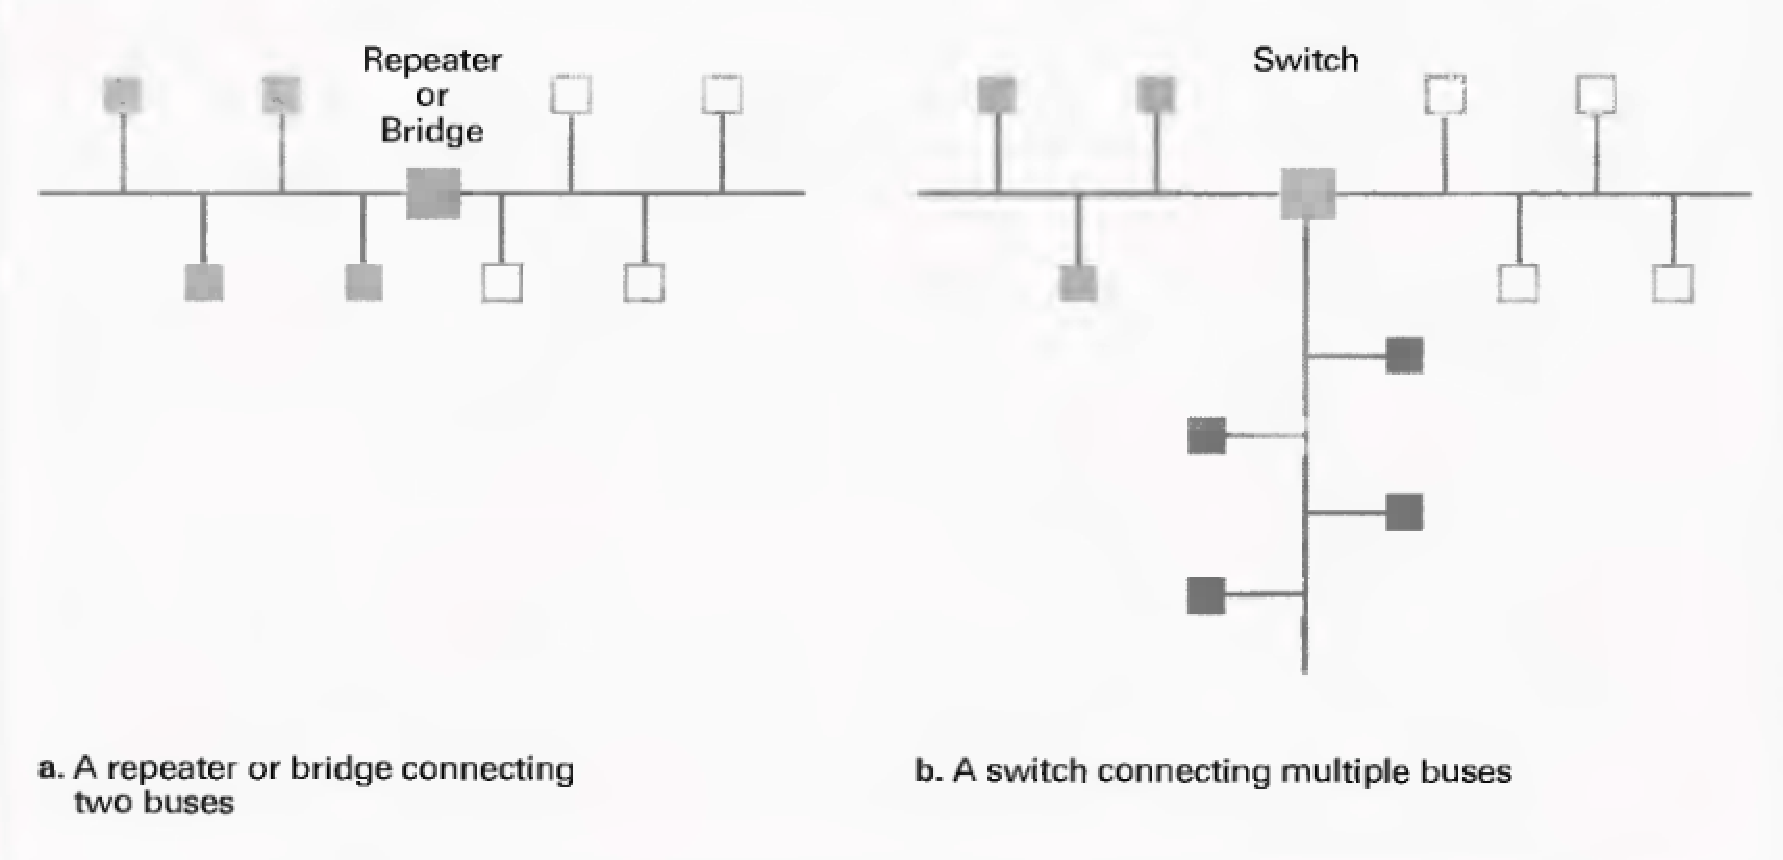
\includegraphics{ch5/fig44.pdf}}
  \caption{Xây dựng một mạng hình tuyến lớn từ những mạng nhỏ hơn}
  \label{fig:fig4.4}
\end{figure}

\textbf{Cầu nối} là một thiết bị tương đương, nhưng phức tạp hơn so với bộ lặp tín
hiệu. Cũng như bộ lặp tín hiệu, cầu nối kết nối hai mạng hình tuyến với nhau, nhưng nó
không nhất thiết phải chuyển tiếp tất cả các thông điệp từ tuyến này sang tuyến kia. Thay
vào đó, nó sẽ xem địa chỉ đích đi kèm với thông điệp và chuyển tiếp thông điệp qua kết nối
chỉ khi thông điệp đó đã được chỉ định trước là sẽ được gửi tới một máy tính ở phía bên
kia của kết nối. Do đó, hai thiết bị nằm ở trên cùng một phía của cầu nối có thể trao đổi
thông điệp mà không gây phiền phức cho sự truyền thông ở phía bên kia của cầu. Cầu nối
thường làm việc có hiệu quả hơn so với bộ lặp tín hiệu.

\textbf{Bộ chuyển mạch} về bản chất là một cầu nối có nhiều cổng kết nối, cho phép nó kết
nối tới nhiều hơn hai tuyến. Do đó, bộ chuyển mạch tạo ra một mạng bao gồm một vài tuyến
được mở rộng từ bộ chuyển mạch như những chiếc nan hoa của bánh xe
(Hình~\ref{fig:fig4.4}b). Cũng giống như cầu nối, bộ chuyển mạch sẽ xem xét địa chỉ đích
của tất cả các thông điệp và chỉ chuyển tiếp những thông điệp nào đã được chỉ định trước
sang các tuyến khác. Hơn nữa, mỗi thông điệp được chuyển tiếp chỉ được chuyển tới các
tuyến tương ứng của địa chỉ đích, chính vì vậy mà nó có thể giảm thiểu được giao thông
trên mỗi tuyến.

Cần phải chú ý rằng khi các mạng được kết nối với những thiết bị như bộ lặp tín hiệu, cầu
nối hay thiết bị chuyển mạch, kết quả là một mạng đơn lớn hơn được tạo ra. Mỗi máy tính
tiếp tục truyền tải thông qua hệ thống theo cách thức cũ (sử dụng cùng một giao thức mạng)
nếu hệ thống được xây dựng ban đầu như là một mạng đơn lớn. Điều đó có nghĩa là, các máy
tính cá nhân trong hệ thống không cần biết đến sự tồn tại của các bộ lặp tín hiệu, các cầu
nối, hay các thiết bị chuyển mạch.

Tuy nhiên, các hệ thống mạng được kết nối đôi khi cũng có những đặc tính không tương thích
nhau. Ví dụ, những đặc tính của mạng vòng tròn sử dụng giao thức thẻ bài vòng tròn
không tương thích với mạng Ethernet hình tuyến sử dụng CSMA/CD. Trong những trường hợp
này, các hệ thống mạng cần phải được kết nối theo một cách thức dùng để tạo ra hệ thống
mạng của các mạng, được biết đến như là hệ thống \textbf{liên mạng} (internet), trong đó
những mạng gốc ban đầu duy trì những tính chất riêng của chúng và tiếp tục vận hành như là
những hệ thống độc lập. (Chú ý rằng \textit{liên mạng (internet)} khác với mạng
\textit{Internet}. Mạng Internet, với chữ cái I được viết hoa, được nói đến như một hệ
thống liên mạng đặc biệt, có phạm vi rộng lớn mà ta sẽ nghiên cứu trong một phần khác của
chương này. Có rất nhiều ví dụ về những hệ thống liên mạng. Quả thực, hệ thống truyền
thông qua điện thoại cổ điển đã được sử dụng khá tốt trong các hệ thống liên mạng phạm vi
rộng trước khi mà mạng Internet được phổ biến.)


\begin{figure}[tb] 
  \centering \scalebox{0.45}{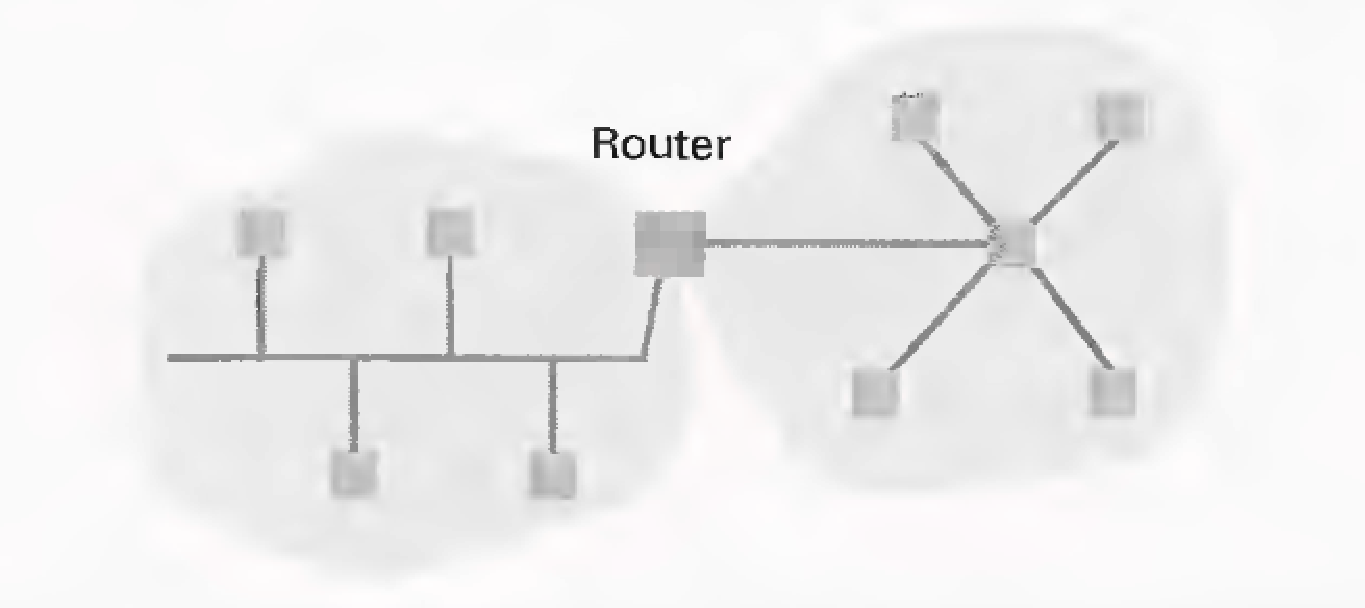
\includegraphics{ch5/fig45.pdf}}
  \caption{Bộ dẫn đường kết nối một mạng hình tuyến với một mạng hình sao tạo thành một hệ
    thống liên mạng}
  \label{fig:fig4.5}
\end{figure}

Sự kết nối giữa hai hệ thống mạng tạo thành một hệ thống liên mạng được thực hiện bởi một
thiết bị gọi là \textbf{bộ dẫn đường} (Router). Một bộ dẫn đường là một máy tính thuộc về
cả hai hệ thống mạng ở hai phía của nó với nhiệm vụ là chuyển tiếp các thông điệp từ mạng
này sang mạng kia (Hình~\ref{fig:fig4.5}). Chú ý rằng nhiệm vụ của bộ dẫn đường đặc biệt
to tát hơn nhiều so với các thiết bị như bộ lặp tín hiệu, cầu nối hay thiết bị chuyển mạch
bởi vì một bộ dẫn đường cần phải thực hiện chuyển đổi giữa các đặc tính riêng biệt của hai
mạng gốc ban đầu. Ví dụ, khi truyền phát một thông điệp từ một mạng sử dụng giao thức thẻ
bài vòng tròn tới một mạng sử dụng giao thức CSMA/CD, bộ dẫn đường phải nhận thông điệp sử
dụng một giao thức sau đó lại sử dụng một giao thức khác để truyền thông điệp đó tới mạng
kia.


Ta sẽ xem xét một ví dụ khác sẽ mô tả sự phức tạp khi thực hiện việc dẫn đường của
Router. Đó là vấn đề khi hai mạng kết nối với nhau lại sử dụng hai hệ thống địa chỉ khác
nhau để xác định các máy tính trong mạng. Khi một máy tính trong một mạng muốn gửi một
thông điệp tới một máy tính ở mạng bên kia, nó không thể xác định được máy tính đích theo
cách thức thông thường mà nó vẫn thường thực hiện.

\begin{figure}[t]
  \begin{quotation}
    \noindent
    \textbf{Mạng Enthernet} \vspace{0.3cm}
    \\
    Mạng Ethernet là một tập các chuẩn được triển khai trong một mạng LAN với mô hình mạng
    hình tuyến. Tên gọi của nó được bắt nguồn từ thiết kế mạng Ethernet ban đầu trong đó
    các thiết bị được kết nối với nhau qua cáp đồng trục. Khởi đầu mạng Ethernet được phát
    triển vào những năm 1970 và ngày nay được chuẩn hóa bởi IEEE là một phần của họ chuẩn
    IEEE 802, mạng Ethernet có hầu hết các cách thức chung của một mạng các máy tính. Việc
    cài đặt các card điều khiển mạng của các máy tính cá nhân trong mạng Ethernet có thể
    thực hiện được và khá dễ dàng.

    Ngày nay trên thực tế có một vài phiên bản của mạng Ethernet với những công nghệ tiên
    tiến hơn và tốc độ truyền tải thông tin cũng cao hơn. Tuy nhiên, tất cả những phiên
    bản mới đó vẫn có đủ các đặc tính chung của họ mạng Ethernet. Mỗi một phiên bản trong
    số đó là một khuôn thức mà trong đó dữ liệu được đóng gói trước khi truyền đi, sử dụng
    mã hóa Manchester (một phương pháp mà trong đó đại diện là các bít 0 và 1, với một bít
    0 sẽ đại diện cho một tín hiệu giảm dần và bít 1 đại diện cho một tín hiệu tăng dần)
    để truyền tải thực sự các bít dữ liệu, và sử dụng giao thức CSMA/CD để điều khiển
    quyền truyền phát.
  \end{quotation}
\end{figure}

Trong những trường hợp như vậy, một hệ thống địa chỉ với phạm vi liên mạng được thiết
lập. Kết quả là mỗi thiết bị trong một hệ thống liên mạng có hai địa chỉ: một địa chỉ của
chính mạng gốc ban đầu của nó và một địa chỉ liên mạng mới. Để gửi một thông điệp từ một
máy tính thuộc một trong những mạng gốc tới một máy tính trong mạng khác--máy tính có địa chỉ
liên mạng của gói tin gốc ban đầu, nó sẽ sử dụng hệ thống địa chỉ gốc của mạng cục bộ để
gửi gói tin tới bộ dẫn đường. Bộ dẫn đường sau đó sẽ xem xét bên trong của gói tin nhận
được, thực hiện tìm địa chỉ liên mạng đích sau cùng của thông điệp, dịch địa chỉ đó thành
địa chỉ có định dạng thích hợp với mạng kia, sau đó chuyển tiếp thông điệp tới đích của
nó. Nói một cách ngắn gọn, các thông điệp trong mỗi một mạng gốc tiếp tục được truyền theo
cách thức của hệ thống địa chỉ gốc của mỗi mạng, và bộ dẫn đường được phân công nhiệm vụ
là chuyển đổi giữa các hệ thống.

\subsection*{Truyền thông liên tiến trình}
Các tiến trình thực thi trên các máy tính khác nhau trong một mạng
máy tính (hay thậm chí trên cùng một máy  theo cách thức chia sẻ thời gian)
thường phải liên lạc với các tiến trình khác  để thực hiện những nhiệm vụ đã được xác định. Việc liên lạc này được gọi là sự \textbf{truyền thông liên tiến trình}.

Một trong những phương thức phổ biến trong truyền thông liên tiến trình là mô hình
\textbf{khách/chủ} (client/server). Mô hình này xác định  vai trò của các tiến
trình trên máy trạm, nơi mà sẽ phát sinh các yêu cầu tới các tiến trình khác trên máy chủ, và các tiến trính trên máy chủ  
nơi sẽ thực hiện các yêu cầu của máy trạm.

Một ứng dụng sơ khai trong mô hình khách/chủ đã xuất hiện trên những mạng liên kết tất cả
máy tính trong một nhóm các văn phòng. Trong tình huống như vậy, một máy in đơn lẻ, chất
lượng cao được kết nối vào mạng nơi mà tất cả các máy tính trong đó có thể sử dụng được
máy in đó. Với trường hợp này máy in đã đóng vai trò của một máy chủ (thường được gọi là
\textbf{máy chủ in} (printer server), và các máy tính khác được lập trình để đóng vai của
các máy trạm sẽ gửi các yêu cầu in ấn tới máy chủ in.

Một ứng dụng khác của mô hình khách/chủ cũng sớm được đưa vào sử dụng nhằm giảm chi phí
lưu trữ bằng cách loại bỏ những nhu cầu về các bản sao trùng lặp của những mẫu tin. Ở đây,
một máy tính trong mạng được trang bị một hệ thống lưu trữ thứ cấp có khả năng cao (thường
sử dụng một đĩa từ) mà trên đó chứa toàn bộ các thông tin dữ liệu của một đơn vị. Các máy
tính khác trên mạng có thể yêu cầu truy cập tới các thông tin dữ liệu mà chúng cần. Khi
đó, máy tính chứa thông tin dữ liệu đóng vai trò là một máy chủ (gọi là \textbf{máy chủ
  file}--file server), và các máy tính khác đóng vai trò là các máy trạm sẽ gửi các yêu
cầu truy cập với những file dữ liệu được lưu trữ trên máy chủ file.

\begin{figure}[tb] 
  \centering \scalebox{0.4}{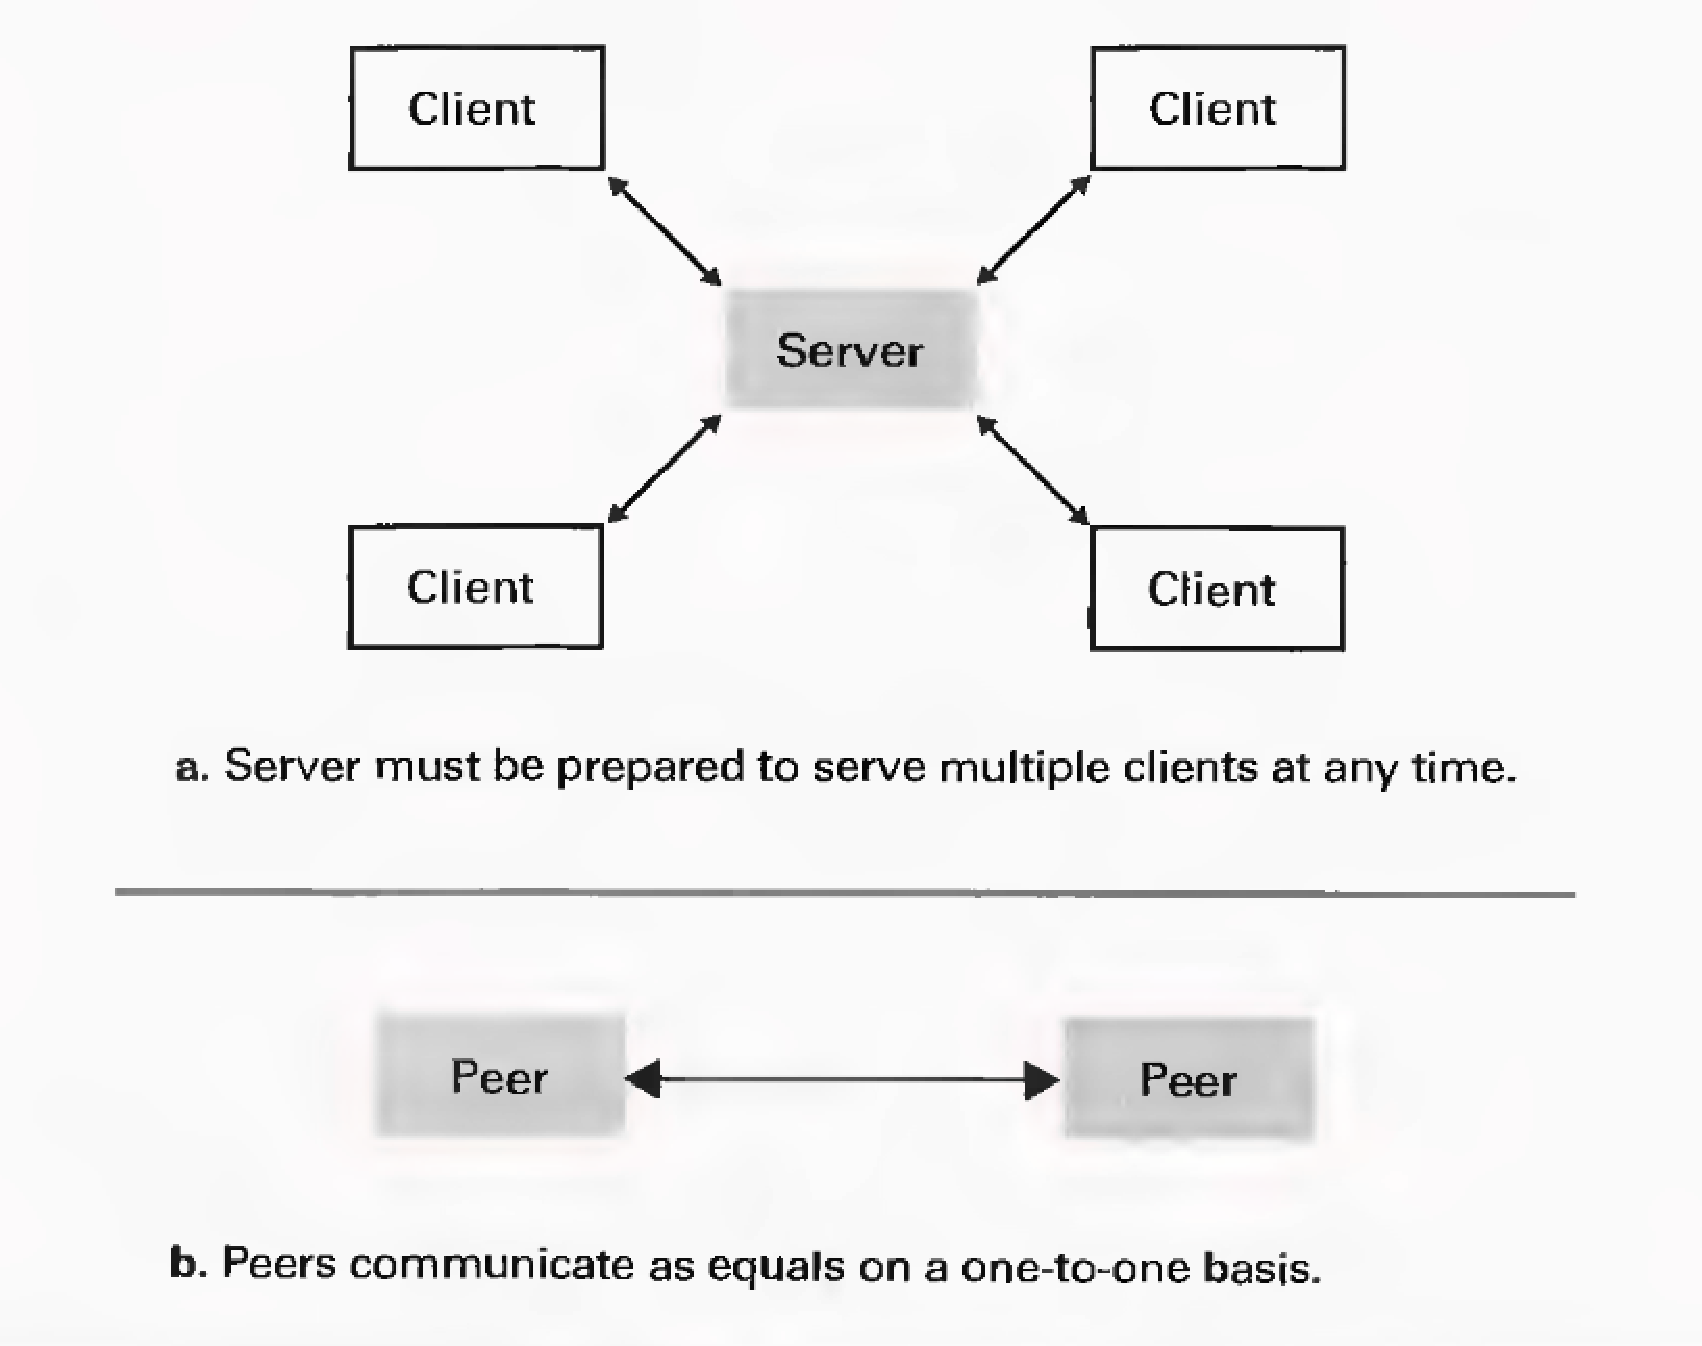
\includegraphics{ch5/fig46.pdf}}
  \caption{Mô hình client/server so sánh với mô hình peer-to-peer}
  \label{fig:fig4.6}
\end{figure}

Ngày nay, mô hình khách/chủ được sử dụng rộng rãi trong các ứng dụng mạng, ta sẽ xem xét ở
phần sau trong chương này. Tuy nhiên, không chỉ mô hình khách/chủ mới hoạt động theo cách
thức như một sự truyền thông liên tiến trình. Một mô hình khác với tên gọi
\textbf{peer-to-peer} (thường được viết tắt là P2P), có những tính chất trái ngược hoàn
toàn với mô hình khách/chủ. Trong khi mô hình khách/chủ bao gồm một tiến trình (trên máy
chủ) thực hiện liên lạc với nhiều tiến trình khác (tại các máy trạm) thì mô hình
peer-to-peer lại bao gồm hai tiến trình trao đổi ngang hàng với nhau
(Hình~\ref{fig:fig4.6}). Ngoài ra, một máy chủ phải chạy liên tục nhằm phục vụ cho các máy
trạm của nó tại bất kỳ thời điểm nào, ngược lại mô hình peer-to-peer với hai tiến trình có
thể thực hiện theo cách thức tạm thời. Ví dụ, các ứng dụng trong mô hình peer-to-peer bao
gồm việc gửi tức thì các thông điệp mà hai người thực hiện đối thoại với nhau qua Internet
cũng như những tình huống như hai người chơi những trò chơi như cờ vua hay cờ đam (một
loại trò chơi gồm 24 quân cờ cho 2 người chơi).


Mô hình peer-to-peer cũng hoạt động theo cách thức chia sẻ file như các bản nhạc hay những
bộ phim qua Internet (đôi khi đi kèm là vấn đề về bản quyền). Trong trường hợp này, những
cá nhân cần tìm kiếm những khoản mục phổ biến có thể quảng bá mong muốn của họ lên
Internet và liên hệ được với những ai sở hữu những khoản mục đó. Sau đó, những khoản mục
này được truyền tải giữa hai phía sử dụng mô hình peer-to-peer. Điều này trái ngược hoàn
toàn với cách tiếp cận của mô hình khách/chủ qua việc thiết lập một ``trung tâm phân
phối'' (máy chủ file) cho các máy trạm tải các bản nhạc (hay ít nhất là tìm thấy các nguồn
của những khoản mục đó). Tuy nhiên, máy chủ trung tâm, đã chứng thực được là một điểm
trung tâm mà tại đó ngành công nghiệp âm nhạc có thể được tuân thủ theo đúng luật bản
quyền, dẫn tới kết quả cuối cùng là sự dỡ bỏ các trung tâm phân phối âm nhạc. Ngược lại,
sự thiếu vắng các trung tâm điều hành như vậy trong mô hình peer-to-peer sẽ khiến nỗ lực
làm cho luật bản quyền có hiệu lực trở nên khó khăn.

Thông thường bạn có thể đọc và nghe về \textit{mạng peer-to-peer}, ví dụ như việc sử dụng
sai những thuật ngữ có thể mắc phải khi những ngôn từ kỹ thuật được thông qua bởi một cộng
đồng phi kỹ thuật. Mạng \textit{peer-to-peer} được biết đến như một hệ thống mà trong đó,
hai tiến trình trao đổi với nhau qua mạng (hoặc liên mạng). Nó không phải là một thuộc
tính của mạng (hay liên mạng). Một tiến trình có thể sử dụng mô hình peer-to-peer để trao
đổi với tiến trình khác thông qua cùng một hệ thống mạng. Vì vậy cần phải nói một cách
chính xác là truyền thông theo cách thức của mô hình peer-to-peer chứ không phải là truyền
thông qua một mạng peer-to-peer.

\subsection*{Các hệ thống phân tán}
Với sự thành công của công nghệ mạng, sự tương tác giữa những máy tính qua các hệ thống
mạng trở nên phổ biến và được thể hiện ở nhiều khía cạnh. Nhiều hệ thống phần mềm hiện
đại, như các hệ thống tìm kiếm hay phục hồi thông tin toàn cầu, các hệ thống kiểm toán có
phạm vi toàn công ty, các trò chơi máy tính, và thậm chí các phần mềm điều khiển chính hệ
thống cơ sở hạ tầng của mạng được thiết kế như là những \textbf{hệ thống phân tán}. Điều
đó có nghĩa là chúng gồm có những đơn vị phần mềm được thực thi dưới dạng các tiến trình trên
các máy tính khác nhau. Ta có thể hình dùng những tiến trình này như là những vị khách cư
trú tại các máy tính khác nhau mà qua đó các máy tính trong một mạng sẽ được gọi là các
\textbf{máy chủ} (host). Điều đó có nghĩa rằng host là một máy tính mà các tiến trình
trú ngụ trên đó theo một hay nhiều ngữ cảnh.

Các hệ thống phân tán đầu tiên được phát triển độc lập từ những hệ thống hỗn tạp. Nhưng
ngày nay, việc nghiên cứu một cách cẩn thận đã cho thấy một cơ sở hạ tầng phổ biến vận
hành trong suốt toàn bộ những hệ thống này, bao gồm cả những thứ như các hệ thống truyền
thông và bảo mật. Đổi lại, kết quả của sự cố gắng đã tạo ra các hệ thống mà có thể cung
cấp cơ sở hạ tầng cơ bản và chính vì vậy, nó cho phép các ứng dụng phân tán được xây dựng
bởi sự phát triển phần hệ thống duy nhất đối với ứng dụng đó.

Một kết quả của nhận định trên là hệ thống đặc tả về giao diện lập trình JavaBeans (được
phát triển bởi Sun Microsystems). Hệ thống này là một môi trường phát triển trợ giúp việc
xây dựng các hệ thống phần mềm phân tán mới. Sử dụng JavaBeans, một hệ thống phân tán được
xây dựng từ những đơn vị được gọi là các bean được tự động thừa kế những đặc tính cơ sở hạ
tầng của hệ thống cha. Do đó, chỉ có những thành phần ứng dụng phụ thuộc duy nhất của một
hệ thống mới mới được phát triển. Một cách tiếp cận khác là môi trường phát triển phần mềm
với tên gọi .NET Framework (được phát triển bởi Microsoft). Với thuật ngữ .NET, các thành
phần của hệ thống phân tán được gọi là các assembly. Mặt khác, bằng việc phát triển các
đơn vị này trong môi trường .NET, chỉ những nét đặc trưng duy nhất đối với một ứng dụng
phổ biến là cần phải được xây dựng dựa trên nền tảng cơ sở hạ tầng có sẵn. Cả hai môi
trường JavaBeans và .NET Framework đều rất đơn giản trong việc phát triển các hệ thống
phần mềm phân tán mới.

\subsection*{Câu hỏi \& Bài tập}

\begin{enumerate}
\item Thế nào là một hệ thống mạng mở?

\item Tóm tắt những đặc tính khác biệt giữa thiết bị lặp tín hiệu và cầu nối

\item Thiết bị dẫn đường là gì?

\item Mô tả một vài mối quan hệ trong xã hội tuân theo mô hình khách/chủ.

\item Mô tả một vài giao thức được sử dụng trong xã hội.

\end{enumerate}



%%% Local Variables: 
%%% mode: latex
%%% TeX-master: "../tindaicuong"
%%% End: 


\section{Mạng Internet}
\label{sec:4.2}
Một trong những hệ thống liên mạng nổi trội nhất đó là mạng \textbf{Internet} (chú ý chữ I
viết hoa), đây là hệ thống mà bắt nguồn từ những dự án nghiên cứu từ những năm 1960 trở về
trước. Mục đích là phát triển khả năng kết nối nhiều mạng máy tính mà chúng có chức năng
như là một hệ thống kết nối không bị phá vỡ bởi những nguy cơ cục bộ. Hầu hết những công
việc ban đầu đều được tài trợ bởi chính phủ Mỹ thông qua Quỹ nghiên cứu Bộ quốc phòng Mỹ
(DARPA - được phát âm là ``DAR-pa''). Trải qua nhiều năm, sự phát triển của mạng Internet
thay đổi (thăng trầm) từ dự án quốc phòng tới dự án nghiên cứu mang tính chất học thuật,
và ngày nay nó được coi là một hệ thống thương mại mà có thể nối kết một tổ hợp các mạng
WAN, MAN, và LAN bao gồm hàng triệu máy tính.

\subsection*{Cấu trúc mạng Internet}
Về khía cạnh khái niệm, mạng Internet có thể được xem như là một tập hợp nhiều
\textbf{miền} (domains), mỗi miền bao gồm một mạng máy tính hay một liên mạng vừa và nhỏ được
điều hành bởi một tổ chức độc lập như một trường đại học, một công ty, hay cơ quan thuộc
chính phủ. Mỗi miền là một hệ thống tự trị (autonomous system) mà có thể được cấu hình với
yêu cầu về mức độ quyền hạn cục bộ. Nó có thể bao gồm một máy tính đơn hay một hệ thống
liên mạng phức tạp có thể bao gồm rất nhiều mạng LAN, MAN, hay thậm chí là mạng WAN.

Sự thành lập của các miền được giám sát bởi \textbf{ICANN (Internet Corporation for
  Assigned Names and Numbers)}, là một tổ chức phi lợi nhuận thực hiện việc thiết lập tên
cho các miền và gán các địa chỉ Internet, ta sẽ xem xét tới vấn đề này ngay sau
đây. Để thành lập một miền trên mạng Internet, miền đó trước tiên phải được đăng ký thông
qua các công ty, gọi là các nhà đăng ký mà đại diện cho tổ chức ICANN.


\begin{figure}[t]
  \begin{quotation}
    \noindent
    \textbf{Internet2} \vspace{0.3cm}
    \\
    Ngày nay mạng Internet đã thay đổi từ một dự án nghiên cứu thành một sản phẩm mang
    tính chất gia đình, cộng đồng nghiên cứu đã chuyển sang một dự án mang tên
    Internet2. Internet2 được mong đợi như là một hệ thống có tính chất học thuật và bao
    gồm rất nhiều các trường đại học làm việc công tác với ngày công nghiệp và chính
    phủ. Mục đích là kiểm soát việc nghiên cứu đối với các ứng dụng liên mạng yêu cầu độ
    rộng dải tần cao trong truyền thông, như hệ thống truy cập và điều khiển từ xa của
    những thiết bị đắt tiền như kính viễn vọng và những thiết bị chẩn đoán trong y tế. Một
    ví dụ của nghiên cứu này là việc thực hiện phẫu thuật từ xa thông qua bàn tay của rô
    bốt bắt chước các cử động của đôi bàn tay của một nhà phẫu thuật ngồi từ xa và quan
    sát bệnh nhân qua băng video. Bạn có thể xem thêm về Internet2 tại địa chỉ \url{
      http://www.internet2.org}
  \end{quotation}
\end{figure}


Khi một miền được đăng ký, nó có thể được gắn vào mạng Internet hiện tại thông qua một bộ
dẫn đường (router) mà kết nối một trong những mạng trong miền tới một mạng đã tồn tại trên
Internet. Bộ dẫn đường đặc biệt này thường được xem như là một cổng vào/ra (gateway) của
miền mà qua đó, nó đại diện cho cổng của miền ra phần còn lại của Internet. Xét trên góc
độ tầm nhìn, nó là một miền đơn lẻ, phần mạng của Internet nằm phía ngoài của cổng vào ra đôi
khi được gọi là đám mây (cloud).

\subsection*{Kết nối tới mạng Internet}

Để đơn giản hóa quá trình kết nối tới mạng Internet, rất nhiều công ty, được gọi là
\textbf{nhà cung cấp dịch vụ Internet (ISP)}, cho phép các khách hàng kết nối những miền
của họ ra ngoài Internet thông qua các thiết bị của ISP hay trở thành một phần của một
miền đã được thiết lập bởi ISP. Có lẽ những cách thức kết nối với chi phí ít tốn kém nhất
tới một ISP vẫn được sử dụng là thông qua các kết nối điện thoại được gọi là kết nối kiểu
quay số (dial-up). Bằng việc sử dụng theo cách thức này, một cá nhân có thể kết nối máy
tính của anh ta hay của cô ta tới đường thoại cục bộ và thực thi một gói phần mềm với
nhiệm vụ gọi đến một máy tính đặt tại ISP. Tại thời điểm đó, ISP cung cấp truy cập
Internet trong suốt thời gian gọi của điện thoại.


\begin{figure}[bth] 
  \centering \scalebox{0.45}{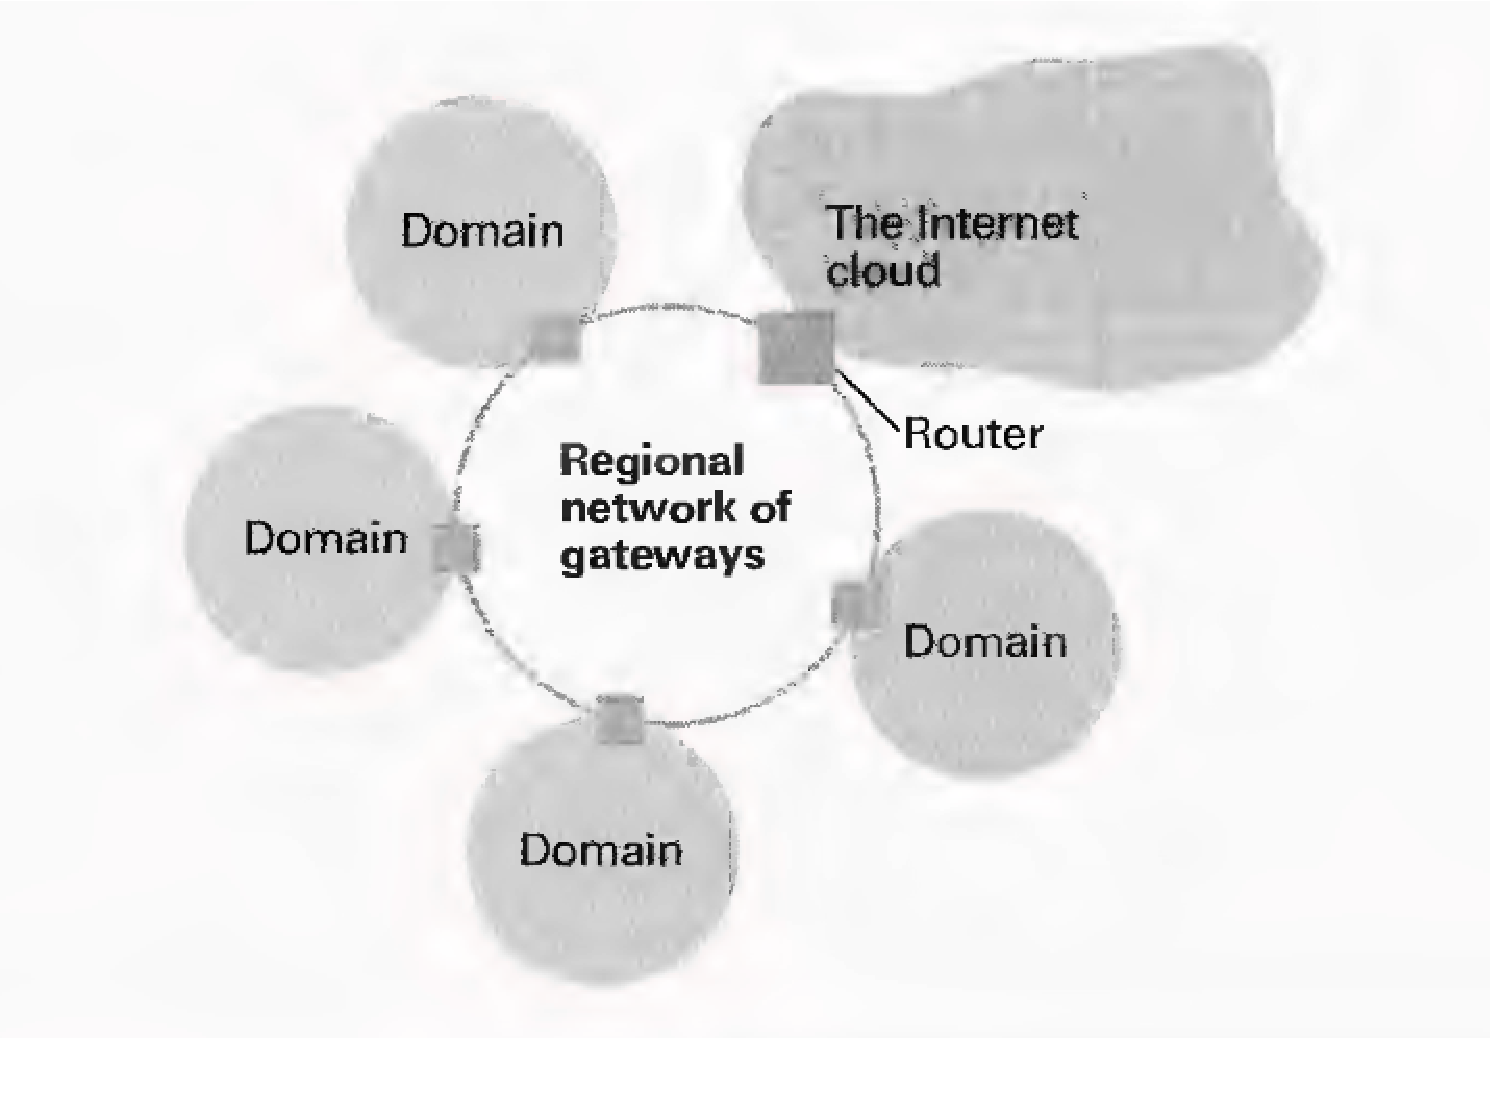
\includegraphics{ch5/fig47.pdf}}
  \caption{ Một cách thức kết nối điển hình tới mạng Internet}
  \label{fig:fig4.7}
\end{figure}

\subsection*{Đánh địa chỉ Internet}
Như đã giới thiệu trong Mục~\ref{sec:4.1}, một liên mạng cần phải được kết hợp với một hệ
thống địa chỉ liên mạng diện rộng mà sẽ gán một địa chỉ xác định cho mỗi máy tính trong hệ
thống. Trong Internet, những địa chỉ này được biết đến như là những \textbf{địa chỉ IP}
(Ký hiệu IP được viết tắt từ cụm “Internet Protocol”, khái niệm mà ta sẽ được giới thiệu
trong Mục~\ref{sec:4.4}). Mỗi địa chỉ IP là một bộ gồm 32 bít và trên thực tế cho đến ngày
nay địa chỉ IP đang trên đà tăng lên thành 128 bít (xem thảo luận về IPv6 trong phần
4.4). Mỗi địa chỉ 32 bít bao gồm hai phần: một phần xác định miền mà trong đó các máy tính
cư trú và một phần xác định mỗi máy tính cụ thể trong miền đó. Phần địa chỉ xác định miền,
được gọi là phần \textbf{định danh mạng}, được gán dưới sự kiểm soát của ICANN tại thời
điểm mà miền đó được đăng ký. Như vậy thông qua quá trình đăng ký này mà mỗi miền trong
mạng Internet được đảm bảo chắc chắn là có một định danh mạng là duy nhất. Phần địa chỉ
xác định một máy tính cụ thể trong miền được gọi là \textbf{địa chỉ máy chủ} (host). Địa
chỉ host được gán bởi người có thẩm quyền trong nội bộ miền đó, thông thường là người có
công việc như quản trị mạng hay quản trị hệ thống.

Địa chỉ IP theo truyền thống được viết thông qua các \textbf{dấu chấm thập phân} ngăn cách
các byte của địa chỉ mà được phân chia theo đoạn và mỗi byte được biểu diễn dưới dạng là
một số nguyên ở dạng thập phân. Ví dụ, sử dụng dấu chấm thập phân, chuỗi 5.2 sẽ được phân
tách thành một chuỗi bít hai byte $0000010100000010$, trong đó bao gồm byte $00000101$
(đại diện cho $5$) và byte liền sau đó là byte $00000010$ (đại diện cho $2$), và chuỗi
$17.12.25$ được biểu diễn thành một chuỗi bít ba byte bao gồm byte $00010001$ (là số $17$
được viết dưới dạng nhị phân), byte sau đó là byte $00001100$ (là số $12$ được viết dưới
dạng nhị phân), và byte cuối cùng là byte $00011001$ (là số $25$ được viết dưới dạng nhị
phân). Như vậy, một máy tính trong miền của Nhà xuất bản~Addison-Wesley có thể có địa chỉ
là $192.207.177.133$, trong đó ba byte đầu tiên ($192.207.177$) được hiểu là định danh cho
mạng (xác định miền Addison-Wesley) và byte cuối cùng ($133$) là địa chỉ host (xác định
một máy tính cụ thể trong miền của Addison-Wesley).

Những địa chỉ dưới dạng bít (thậm chí ngay cả khi được phân tách bằng các dấu chấm thập
phân) rất khó gần gũi theo cách nhận biết của ta. Chính vì lý do này mà mỗi miền cũng được
gán một địa chỉ dễ nhớ hơn được biết đến là \textbf{tên miền} (domain name). Ví dụ, tên
miền của Nhà xuất bản Addison-Wesley là \texttt{aw.com}. Chú ý rằng hệ thống tên miền cũng
phản ánh sự phân loại của miền đó, trong trường hợp này một tổ chức thương mại sẽ được chỉ
định bởi hậu tố \texttt{com}. Sự phân loại này được xem như là miền có \textbf{cấp cao
  nhất} (TLD: top-level domain). Có rất nhiều TLD, bao gồm \texttt{edu} cho các lĩnh vực
liên quan đến giáo dục, \texttt{gov} đại diện cho các cơ quan chính phủ Mỹ, \texttt{info}
đại diện cho mục đích sử dụng không hạn chế, và \texttt{net}, được mong đợi dành cho những
nhà cung cấp dịch vụ Internet nhưng ngày nay lại được sử dụng trong rất nhiều lĩnh vực
khác. Bên cạnh những TLD, còn có các ký hiệu hai ký tự TLD đại diện cho các quốc gia (được
gọi là TLD mã quốc gia), ví dụ như \texttt{au} đại diện cho Australia và \texttt{ca} đại
diện cho Canada.

Khi một miền có một tên dễ nhớ, người có quyền trong nội bộ miền đó có thể tùy ý mở rộng
đặt các tên dễ nhớ cho các máy tính trong miền của mình. Ví dụ, một máy tính cá nhân trong
miền \texttt{aw.com} có thể được xác định qua tên \url{ssenterprise.aw.com}.

Ta cần phải nhấn mạnh rằng dấu chấm thập phân được sử dụng trong những địa chỉ dễ
nhớ không liên quan gì với những dấu chấm thập phân được dùng trong địa chỉ IP. Thay vào
đó, những phần trong một địa chỉ dễ nhớ xác định vị trí của một máy tính trong một hệ
thống phân cấp có thứ bậc. Nói một cách cụ thể, địa chỉ \url{ssenterprise.aw.com} chỉ ra
máy tính \texttt{ssenterprise} là nằm trong tổ chức \texttt{aw}, \texttt{aw} nằm trong lớp
(hay TLD) của những miền thương mại \texttt{com}. Trong trường hợp những miền lớn, người
có quyền trong nội bộ miền đó có thể chia nhỏ miền lớn thành những miền con (subdomain),
trong đó những địa chỉ dễ nhớ đại diện cho các máy tính trong miền có thể được đặt dài
hơn. Ví dụ, đại học Nowhere được gán một tên miền là \url{nowhereu.edu} và chọn lựa chia
miền lớn thành nhiều miền con. Khi đó, một máy tính tại đại học Nowhere có thể có một địa
chỉ như \url{r2d2.compsc.nowhereu.edu}, điều này có nghĩa là máy tính r2d2 là thuộc miền
con \texttt{compsc} nằm trong miền \texttt{nowhereu} nằm trong lớp miền thuộc lĩnh vực
giáo dục \texttt{edu}.

Mỗi người có quyền nội bộ trong miền của mình có trách nhiệm duy trì một danh mục chứa địa
chỉ dễ nhớ và địa chỉ IP tương ứng của những máy tính trong miền đó. Danh mục này được
triển khai trên một máy tính ủy quyền trong miền dưới dạng là một máy chủ (server), được
gọi là \textbf{máy chủ tên miền}, có nhiệm vụ đáp ứng lại với những yêu cầu về thông tin
địa chỉ. Tất cả các máy chủ tên miền ở khắp nơi trên Internet là thành phần của một hệ
thống danh mục mạng Internet diện rộng được biết đến như \textbf{hệ thống tên miền} (DNS:
domain name system) được sử dụng để chuyển đổi địa chỉ từ dạng dễ nhớ sang dạng bít tương
đương. Cụ thể là khi một người gửi yêu cầu cần xác định tới một đích ở dạng dễ nhớ thông
qua một thông điệp, DNS được sử dụng để chuyển đổi địa chỉ dễ nhớ đó sang dạng địa chỉ IP
tương đương mà tương thích với các ứng dụng Internet. Quá trình bóc tách thông tin từ DNS
thường được hiểu như là quá trình ``tra cứu DNS'' (DNS lookup). Thông thường, một tra cứu
DNS được hoàn thiện trong một phần của giây.


\subsection*{Các ứng dụng trên mạng Internet}
Trong phần này ta sẽ thảo luận về ba ứng dụng truyền thống của mạng Internet, và
trong phần tiếp theo ta sẽ khám phá ứng dụng thứ tư của nó. Ta xem xét những
ứng dụng truyền thống này vì chúng đề cập tới quy ước giao tiếp giữa các máy tính với nhau
trên mạng Internet. Tuy nhiên, ngày nay, sự khác biệt giữa một máy tính và các thiết bị
điện tử khác cũng trở nên không rõ ràng nhiều. Điện thoại, vô tuyến truyền hình, các hệ
thống âm thanh, chuông báo trộm, lò vi sóng, và cả máy quay video, tất cả đều trở thành
các máy tính và có xu hướng trở thành các ``thiết bị Internet''. Ngược lại, những ứng dụng
truyền thống của mạng Internet hầu hết có thể bị làm cho lạc hậu bởi một sự tràn lan mở
rộng của những thói quen tập tục mới, minh họa là sự mở rộng nhanh chóng của lĩnh vực điện
thoại Internet với tên gọi là \textbf{voice over Internet} (hay với những tên gọi thiên về
kỹ thuật hơn như \textbf{voice over IP}, viết tắt là \textbf{VoIP}), với cách thức truyền
dữ liệu thoại đơn giản qua Internet thay vì qua hệ thống mạng điện thoại truyền thống.

Với sự phân tích cuối cùng, mạng Internet chỉ đơn thuần là một hệ thống truyền thông mà dữ
liệu có thể được truyền tải qua đó. Khoa học kỹ thuật tiếp tục làm tăng tốc độ truyền của
hệ thống, nội dung dữ liệu được truyền tải sẽ bị giới hạn chỉ bởi sức tưởng tượng của một
ai đó--điện thoại và sóng vô tuyến là sự xác thực đúng đắn.

Tuy nhiên, bay giờ ta hãy xem xét ba ứng dụng sơ đẳng ``hướng máy tính'' của mạng
Internet.

\paragraph{Thư điện tử (Electronic Mail)} Một trong những thói quen phổ biến nhất trên
mạng Internet là \textbf{thư điện tử} (email - viết tắt của từ electronic mail), một hệ
thống mà trong đó các thông điệp được truyền tải giữa những người sử dụng Internet. Nhằm
phục vụ cho mục đích của dịch vụ cung cấp thư điện tử, mỗi người quản lý miền cục bộ của
mình được chỉ định một máy tính đặc biệt mà trong đó miền của nó điều khiển các hoạt động
thư điện tử. Máy tính này được biết đến như là một \textbf{máy chủ thư} của miền (mail
server). Với mỗi thông điệp thư điện tử được gửi từ bên trong của miền, trước tiên phải
được gửi tới máy chủ thư của miền, sau đó nó sẽ gửi thông điệp này tới đích của thông
điệp. Tương tự như vậy, mỗi thông điệp thư điện tử được đánh địa chỉ gắn với một người
trong miền sẽ được nhận bởi máy chủ thư của miền, nơi mà thông điệp sẽ được giữ lại đó cho
đến khi một ai đó yêu cầu xem thư đến (incoming mail) của anh ta hay cô ta.

Với vai trò của máy chủ thư của miền, có thể dễ dàng hiểu được cấu trúc của một địa chỉ
thư điện tử của một cá nhân nào đó. Nó bao gồm một chuỗi ký tự (đôi khi được gọi là tên
tài khoản) xác định một cá nhân duy nhất, sau đó là ký tự \texttt{@} (đọc là ``at''), sau
đó là chuỗi tên dễ nhớ mà đại diện cho máy chủ thư nơi có thể nhận được thư. (Trên thực
tế, chuỗi này thường chỉ đơn thuần xác định miền đích, và máy chủ thư của miền là định
danh cơ bản lấy được từ quá trình tra cứu DNS). Như vậy địa chỉ thư điện tử của một cá
nhân lại Nhà xuất bản~Addison-Wesley có thể sẽ là \url{shakespeare@aw.com}. Nói cách khác,
một thông điệp được gửi tới địa chỉ này thì sẽ đi tới máy chủ thư nằm trong miền aw.com
nơi mà nó có thể được nắm giữ bởi một người có định danh là một chuỗi ký
tự~\texttt{shakespeare}.

\begin{figure}[t]
  \begin{quotation}
    \noindent
    \textbf{POP3 so sánh với IMAP} \vspace{0.3cm}
    \\
    Những người sử dụng trên mạng Internet sử dụng dịch vụ thư điện tử thông qua những kết
    nối từ xa tạm thời tới nhà cung cấp Internet của họ có thể cũng đã nghe nói, và có lẽ
    nhận được một sự lựa chọn giữa, POP3 (đánh vần là ``pop-BA'') và IMAP (đánh vần là
    ``AI-mép''). Đây là những giao thức mà qua đó một người dùng tại một máy tính từ xa
    (có thể là một máy tính xách tay hay một thiết bị cầm tay PDA) có thể truy cập vào các
    thông điệp mà đã thu thập được qua một máy chủ thư và lưu trữ trong hòm thư của người
    dùng đó. POP3 là chữ viết tắt của cụm từ Post Office Protocol--version 3 và đơn giản
    hơn hai. Thông qua việc sử dụng POP3, người dùng truyền (tải) các thông điệp tới máy
    tính cục bộ của anh ta hay cô ta nơi mà họ có thể đọc, lưu trữ vào nhiều thư mục khác
    nhau, sửa đổi, và những thao tác khác tùy theo mong muốn của người dùng. Hành động này
    được thực hiện trên máy tính cục bộ của người dùng qua việc sử dụng bộ nhớ thứ cấp của
    máy tính đó. IMAP, viết tắt của cụm từ Internet Mail Access Protocol, cho phép một
    người dùng lưu trữ và thao tác trên các thông điệp và những tài nguyên liên quan trên
    chính máy chủ thư. Theo cách thức này, một người dùng phải truy cập vào thư điện tử
    của anh ta hay cô ta từ những máy tính khác nhau có thể vẫn duy trì những bản ghi trên
    máy chủ thư và sau đó có thể sử dụng thông qua bất kỳ một máy tính từ xa nào mà người
    dùng đó có thể truy cập. Do đó, IMAP cung cấp một cấp độ dịch vụ cao hơn từ phía ISP
    trong việc duy trì máy chủ thư, và chính vì vậy mà ISP có thể đòi trả một mức phí cao
    hơn đối với dịch vụ IMAP khi so sánh với POP3.
  \end{quotation}
\end{figure}

\paragraph{Giao thức truyền tệp (File Transfer Protocol)} Một cách thức truyền tải các tệp
(ví dụ như văn bản, ảnh, hay những thông tin được mã hóa khác) là đính kèm chúng vào các
thông điệp thư điện tử. Tuy nhiên, một phương pháp hiệu quả hơn là tận dụng được lợi ích
của\textbf{ giao thức truyền tệp} (FTP), là giao thức khách/chủ cho phép truyền tải các
tệp qua mạng Internet. Để truyền một tệp sử dụng FTP, một người dùng từ một máy tính nào
đó trên mạng Internet sử dụng một gói phần mềm cho phép thi hành FTP nhằm thiết lập một
kết nối với một máy tính khác. (Máy tính gốc đóng vai trò là máy khách. Máy tính mà nó kết
nối tới đóng vai trò là một máy chủ, thường được gọi là máy chủ FTP.)  Khi kết nối này
được thiết lập, các tệp có thể được truyền tải giữa hai máy tính theo một trong hai hướng.

FTP đã trở thành một cách thức cung cấp truy cập hạn chế tới dữ liệu phổ biến qua mạng
Internet. Ví dụ như bạn muốn cho phép một người nào đó truy cập được tới một tệp trong khi
những người khác lại không được phép. Bạn chỉ cần đặt tệp đó trên một máy tính có khả năng
như một máy chủ FTP và thiết lập quyền truy cập tới tệp thông qua một mật khẩu. Sau đó,
người nào biết được mật khẩu đó sẽ có thể đạt được quyền truy cập tới tệp thông qua FTP,
trong khi những người khác thì bị chặn lại. Một máy tính trên mạng Internet được sử dụng
theo cách tương tự đôi khi được gọi là các site FTP bởi vì nó tạo thành một vị trí trên
mạng Internet mà tại đó các tệp có thể được truyền tải thông qua FTP.

Các FTP site cũng thường cung cấp quyền truy cập không hạn chế tới các tệp. Để thực hiện
được điều này, các máy chủ FTP sử dụng một khoản mục \textit{nặc danh} (anonymous) như là
một tên đăng nhập thông thường. Những site như vậy thường được xem như là những site
\textbf{FTP nặc danh} và cung cấp quyền truy cập tệp không hạn chế dưới sự đỡ đầu của
chúng.

Một đặc tính rất dễ bị hiểu nhầm của FTP là sự khác biệt mà nó tạo ra giữa những ``tệp văn
bản'' và ``tệp nhị phân''. Căn nguyên của sự khác biệt này là khi in một tệp văn bản với
những thiết bị điện báo đánh chữ đời đầu, một dòng văn bản mới yêu cầu phải có cả hai ký
tự xuống dòng (di chuyển theo chiều dọc) và ký tự về đầu dòng (di chuyển theo chiều
ngang), mỗi ký tự đó được mã hóa riêng biệt theo mã ASCII. (Một ký tự xuống dòng được chỉ
ra qua chuỗi nhị phân $00001010$, trong khi một ký tự về đầu dòng được biểu diễn dưới dạng
một chuỗi nhị phân là $00001101$.) Nhằm đạt được mục đích hiệu quả, rất nhiều nhà lập
trình ban đầu đã tìm ra nó thuận tiện trong việc đánh dấu những ngắt dòng trong một tệp
văn bản với chỉ một trong những mã này. Ví dụ, nếu một ai đó đồng ý đánh dấu ngắt dòng với
chỉ một ký tự về đầu dòng hơn là dùng cả hai ký tự về đầu dòng và xuống dòng, khi đó, tám
bít của khoảng trống trong tệp sẽ được lưu trữ cho mỗi dòng văn bản trong tệp đó. Cần nhớ
rằng phải chèn ký tự xuống dòng cho mỗi lần gặp ký tự về đầu dòng khi thực hiện in tệp
đó. Những cách thức nhanh chóng (vắn tắt) này vẫn còn tiếp tục tồn tại trong nhiều hệ
thống ngày nay. Cụ thể là hệ điều hành UNIX thừa nhận rằng ký tự ngắt dòng trong một tệp
văn bản được chỉ ra chỉ là ký tự xuống dòng, trong khi những hệ thống được phát triển bởi
công ty Apple Computer, lại sử dụng ký tự về đầu dòng, và hệ điều hành của Microsoft lại
yêu cầu cả hai ký tự về đầu dòng và xuống dòng. Kết quả là khi những tệp này được truyền
từ một hệ thống này sang một hệ thống khác, cần phải thiết lập những quá trình chuyển đổi.

Chính điều này đã dẫn tới sự khác biệt giữa ``tệp văn bản'' và ``tệp nhị phân'' trong
FTP. Nếu một tệp là ``tệp văn bản'' được truyền đi sử dụng FTP, quá trình chuyển đổi theo
yêu cầu sẽ được tạo ra như là một phần của quá trình truyền; nếu tệp cần truyền là ``tệp
nhị phân'', không có quá trình chuyển đổi nào cần phải tạo ra. Chính vì vậy mà thậm chí
cho dù bạn có thể nghĩ rằng một tệp được tạo ra bởi một bộ xử lý văn bản dưới dạng tệp văn
bản, nó không thể truyền như là một ``tệp văn bản'' khi những tệp này sử dụng những mã đại
diện cho ký tự xuống dòng và về đầu dòng thuộc quyền sở hữu riêng của bộ xử lý văn
bản. Nếu một ``tệp nhị phân'' ngẫu nhiên được truyền dưới dạng như là một ``tệp văn bản'',
nó sẽ gặp những vấn đề biến đổi không lường trước.

\paragraph{Telnet và Secure Shell} Một trong những thói quen sơ khai trên mạng Internet là
cho phép người dùng máy tính truy cập vào các máy tính khác từ một khoảng cách
xa. \textbf{Telnet} là một hệ giao thức mà qua đó có thể thực hiện được cho mục đích
này. Qua telnet, một người dùng (chạy phầm mềm telnet khách) có thể liên lạc với máy chủ
telnet tại một máy tính từ xa và sau đó theo quy trình đăng nhập của hệ điều hành, người
dùng sẽ đạt được quyền truy cập vào máy chủ đó.

Tất cả sự liên lạc qua telnet được thực hiện dưới dạng là thông qua một thiết bị ảo, được
gọi là Network Virtual Terminal (NVT), mà theo cách tưởng tượng độc đáo thì đó như là một
bàn phím và một máy in. Giao thức telnet định nghĩa một tập các lệnh cho việc truyền các
ký tự tới và từ một thiết bị ảo như vậy. Tất cả các máy chủ telnet đều được thiết kế nhằm
cho phép người dùng liên lạc được thông qua các câu lệnh này ngay cả khi chúng giao tiếp
với một NVT. Ngược lại, tất cả các máy khách phải thực hiện liên lạc với một máy chủ
telnet với tư cách như là một NVT. Chính vì vậy, nhiệm vụ của một máy khách telnet là phải
chuyển đổi những đặc tính riêng trong hệ thống cục bộ của nó nhằm thích ứng được với những
thuộc tính của một NVT.

Do được thiết kế vào những thời gian đầu trong quá trình phát triển của mạng Internet nên
telnet cũng có một vài điều thiếu sót. Một trong những lời lẽ chỉ trích đó là cho rằng
thông tin liên lạc qua telnet là không được mã hóa. Điều này rất có ý nghĩa cho dù chủ đề
của sự liên lạc là không dễ dàng bị tác động bởi vì mật khẩu của người dùng cũng là một
phần của sự liên lạc đó trong suốt quá trình đăng nhập. Do đó thói quen sử dụng telnet
cũng mở ra khả năng cho một người nghe trộm có thể chặn được mật khẩu và sau đó sử dụng
sai mục đích những thông tin nghiêm trọng này. \textbf{Secure Shell (SSH)} là một hệ thống
liên lạc đưa ra được một giải pháp cho vấn đề này và đã nhanh chóng thay thế vị thế của
telnet. Một trong những đặc tính của SSH là nó cung cấp khả năng mã hóa dữ liệu khi được
truyền cũng như khả năng xác thực thông tin (Mục~\ref{sec:4.5}), và trên thực tế đó cũng
là quá trình tạo dựng sự chắc chắn cho việc hai bên đang liên lạc với nhau như chúng khẳng
định.

\subsection*{Câu hỏi \& Bài tập}


\begin{enumerate}
\item Sự khác nhau giữa một định danh mạng và địa chỉ host là gì?
\item Nêu những thành phần của một địa chỉ Internet của một máy tính?
\item Chuỗi bít đại diện cho $3.4.5$ với ký hiệu dấu chấm thập phân là gì?  Biểu diễn
  chuỗi bít $0001001100010000$ sử dụng ký hiệu dấu chấm thập phân.
\item Theo cách nào thì cấu trúc của một địa chỉ dễ nhớ của một máy tính trên mạng
  Internet (ví dụ như \url{r2d2.compsc.nowhereu.edu}) tương đương như một địa chỉ bưu điện
  truyền thống? Cấu trúc tương tự này có xảy ra đối với địa chỉ IP không?
\item Nêu tên ba loại máy chủ trên mạng Internet và kể về mỗi loại đó.
\item Tại sao SSH lại được xem là tốt hơn so với telnet?
\end{enumerate}









%%% Local Variables: 
%%% mode: latex
%%% TeX-master: "../tindaicuong"
%%% End: 


\section{World Wide Web}

Trong phần này ta sẽ tập trung vào thảo luận về một ứng dụng trên mạng Internet mà
nhờ nó thông tin đa phương tiện có thể được phổ biến thông qua mạng Internet. Nó được dựa
trên khái niệm về \textbf{siêu văn bản} (hypertext), một cụm từ mô tả những tài liệu dạng
văn bản mà trong đó có chứa các liên kết, với tên gọi là \textbf{các siêu liên kết}
(hyperlinks), hay chứa những văn bản khác. Ngày nay, siêu văn bản đã mở rộng ra và có thể
bao gồm cả hình ảnh, âm thanh và video, và cũng chính sự mở rộng phạm vi này mà đôi khi nó
còn được gọi là \textbf{siêu phương tiện} (hypermedia).

Khi sử dụng một giao diện đồ họa (GUI), người đọc một tài liệu siêu văn bản có thể lần
theo những siêu liên kết trong tài liệu bằng cách kích chuột vào nó. Ví dụ, giả sử câu
``Sự trình diễn nhạc qua điệu nhảy ‘Bolero’ bởi Maurice Ravel rất ấn tượng'' xuất hiện
trong một tài liệu siêu văn bản và tên \textit{Maurice Ravel} được liên kết tới một tài
liệu khác--có thể cho ta thông tin về nhà soạn nhạc đó. Một người đọc có thể chọn xem
thông tin liên quan đó bằng cách di chuyển trỏ chuột vào tên \textit{Maurice Ravel} và
kích vào nút chuột. Ngoài ra, nếu những siêu liên kết thích ứng được cài đặt, người đọc có
thể nghe được một bản ghi âm của buổi hòa nhạc bằng cách kích chuột vào tên
\textit{Bolero}.

Theo cách đó, một người đọc những tài liệu siêu văn bản có thể khai thác được những tài
liệu liên quan hay lần theo chuỗi từ tài liệu này đến tài liệu khác. Khi nhiều phần khác
nhau của các tài liệu được liên kết tới những tài liệu khác, một mạng lưới thông tin liên
quan với nhau được hình thành. Khi triển khai trên một mạng máy tính, các tài liệu trong
đó như một mạng lưới có thể thường trú trên nhiều máy tính khác nhau, dạng như một lưới
mạng diện rộng. Mạng lưới mà đã phát triển trên mạng Internet mở rộng ra phạm vi toàn cầu
và được biết đến với tên gọi là World Wide Web (thường được viết tắt là \textbf{WWW},
\textbf{W3} hay \textbf{Web}). Một tài liệu siêu văn bản trên World Wide Web thường được
gọi là một \textbf{trang Web} (Web page). Một tập hợp những trang Web có mối quan hệ gần
nhau được gọi là một \textbf{website}.

World Wide Web có nguồn gốc khởi đầu là từ công việc của Tim Berners-Lee, người đã nhận ra
được tiềm năng của việc kết hợp khái niệm liên kết tài liệu với công nghệ liên mạng và đã
đưa ra được phần mềm đầu tiên là việc triển khai WWW vào tháng 12 năm 1990.

\subsection*{Triển khai Web}

Những gói phần mềm cho phép người sử dụng truy cập tới những siêu văn bản trên mạng
Internet thuộc về một trong hai loại: những gói đóng vai trò là những ứng dụng khách, và
những gói đóng vai trò là những ứng dụng phục vụ. Một gói ứng dụng khách thường được đặt
trên máy tính của người sử dụng và được giao nhiệm vụ thu nạp các tài liệu mà được yêu cầu
từ phía người dùng, sau đó trình diễn những tài liệu này cho người dùng xem theo một cách
thức có tổ chức. Ứng dụng khách mà cung cấp giao diện người dùng cho phép một người sử
dụng có thể duyệt qua lại trên Web. Do đó những ứng dụng khách dạng như vậy thường được
gọi là \textbf{trình duyệt} (browser), hay đôi khi còn được gọi là trình duyệt Web. Gói
ứng dụng trên máy chủ (thường gọi là \textbf{ứng dụng phục vụ Web} (Web server)) thường
trú trên một máy tính chứa các tài liệu siêu văn bản sẽ được truy cập tới. Nhiệm vụ của nó
là cung cấp quyền truy cập tới các tài liệu trên nó khi có yêu cầu từ phía các ứng dụng
khách. Nói tóm lại, một người dùng giành được quyền truy cập tới các tài liệu siêu văn bản
thông qua một trình duyệt thường trú trên máy tính của người dùng đó. Trình duyệt này,
đóng vai trò là một ứng dụng khách, thu nạp các tài liệu bằng cách gửi các yêu cầu về dịch
vụ tới các máy chủ Web nằm rải rác trên mạng Internet. Các tài liệu siêu văn bản thông
thường được truyền qua lại giữa các trình duyệt và máy chủ Web sử dụng một giao thức được
biết đến là \textbf{Giao thức Truyền Siêu văn bản} (HTTP: Hypertext Transfer Protocol).

Để có thể định vị và truy nạp các tài liệu trên World Wide Web, mỗi tài liệu được gắn vào
nó là một địa chỉ duy nhất với tên gọi là Địa chỉ \textbf{Uniform Resource
  Locator(URL)}. Mỗi URL chứa thông tin cho phép một trình duyệt liên lạc được tới một máy
chủ tương ứng và yêu cầu nạp tài liệu mong muốn. Do đó, khi xem một trang Web, một người
nào đó trước tiên cần phải cung cấp cho trình duyệt URL của tài liệu mà anh ta hay cô ta
cần nạp và sau đó ra lệnh cho trình duyệt nạp và hiển thị tài liệu đó lên.

\begin{figure}[bt] 
  \centering \scalebox{0.45}{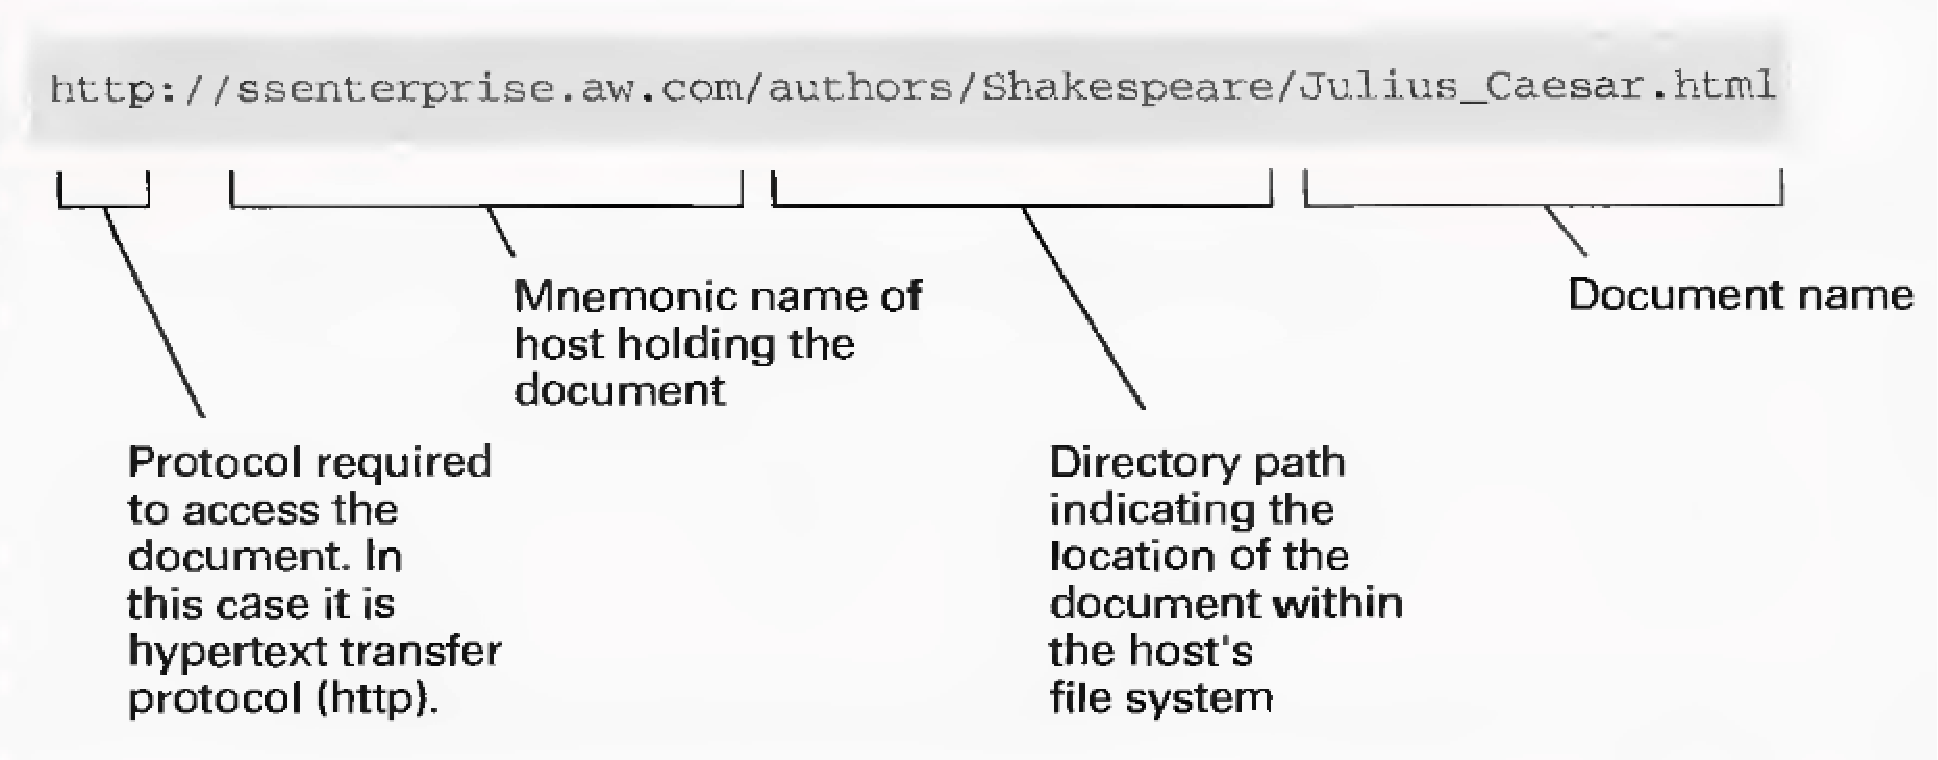
\includegraphics{ch5/fig48.pdf}}
  \caption{Một URL đặc trưng}
  \label{fig:fig4.8}
\end{figure}

Một URL đặc trưng được biểu diễn qua Hình~\ref{fig:fig4.8}. Nó bao gồm bốn phần: giao thức
được sử dụng để giao tiếp với ứng dụng trên máy chủ điều khiển truy cập tới tài liệu, địa
chỉ dễ nhớ của máy tính chứa ứng dụng chủ, đường dẫn cần cho ứng dụng chủ tìm tới thư mục
chứa tài liệu, và cuối cùng là tên của tài liệu. Nói một cách ngắn gọn, URL trong
Hình~\ref{fig:fig4.8} chỉ ra rằng một trình duyệt liên lạc tới một ứng dụng phục vụ Web
đặt trên một máy tính được biết đến là \url{ssenterprise.aw.com} sử dụng giao thức HTTP để
thu nạp tài liệu tên là \texttt{Julius\_Caesar.html} được đặt trong thư mục con
\texttt{Shakespeare} trong thư mục \texttt{authors}.

Đôi khi một URL có thể không nhất thiết phải chứa đủ cả các thành phần được chỉ ra trong
Hình~\ref{fig:fig4.8}. Ví dụ, nếu ứng dụng chủ không cần phải lần theo một đường dẫn thư
mục tới tài liệu, khi đó sẽ không có đường dẫn xuất hiện trong URL nữa. Ngoài ra, đôi khi
một URL sẽ bao gồm chỉ một giao thức và địa chỉ dễ nhớ của một máy tính. Trong trường hợp
này, ứng dụng phục vụ Web tại máy tính đó sẽ trả về một tài liệu được chỉ định trước,
thông thường được gọi là trang chủ (home page), mà thường mô tả thông tin sẵn có trên
website đó. Những URL được làm ngắn gọn như vậy cung cấp một cách thức đơn giản để liên
lạc được với các tổ chức. Ví dụ, URL \url{http://www.aw.com} sẽ dẫn tới trang chủ của Nhà
xuất bản~Addison-Wesley, mà trên đó có chứa các siêu liên kết tới rất nhiều các tài liệu
khác liên quan đến nhà xuất bản và các sản phẩm của họ.

Nhằm đơn giản hóa việc định vị các website, rất nhiều trình duyệt mặc định hiểu rằng giao
thức HTTP sẽ được sử dụng nếu không có giao thức nào được chỉ định. Những trình duyệt này
có thể nạp chính xác trang chủ của Addison-Wesley khi nhận được yêu cầu nạp từ ``URL'' bao
gồm chỉ đơn thuần là \url{www.aw.com}.

Tất nhiên, một người sử dụng Web có thể cần phải tìm kiếm về một chủ đề nào đó hơn là truy
nạp một tài liệu cụ thể. Với mục đích này, rất nhiều website (bao gồm cả các trang chủ của
hầu hết các ISP) cung cấp các dịch vụ của một phương tiện tìm kiếm. Một \textbf{phương
  tiện tìm kiếm} là một gói phần mềm được thiết kế nhằm trợ giúp cho người sử dụng Web xác
định các tài liệu liên quan tới các chủ đề khác nhau. Để sử dụng một phương tiện tìm kiếm,
người sử dụng cần gõ một tập các từ hay cụm từ mà tài liệu mong muốn tìm được có thể chứa
chúng, sau đó phương tiện tìm kiếm sẽ quét toàn bộ các bản ghi của nó, đưa ra báo cáo về
các tài liệu mà nội dung có chứa văn bản cần xác định. Việc cải tiến công nghệ cho các
phương tiện tìm kiếm, bao gồm những phương pháp tốt hơn cho việc xác định các tài liệu
liên quan và cải tiến những hệ thống xây dựng và lưu trữ những bản ghi nằm trong hệ thống
tìm kiếm, đang là một quá trình tiếp diễn.


\begin{figure}[t]
  \begin{quotation}
    \noindent
    \textbf{World Wide Web Consortium} \vspace{0.3cm}
    \\
    The World Wide Web Consortium (W3C) được hình thành vào năm 1994 nhằm đẩy mạnh World
    Wide Web bằng cách phát triển các quy ước chuẩn (được biết đến là các chuẩn W3C). Trụ
    sở W3C được đặt tại CERN, phòng thí nghiệm vật lý hạt nhân năng lượng cao tại Geneva,
    Thụy Sĩ. CERN là nơi mà ngôn ngữ đánh dấu HTML gốc được phát triển theo giao thức HTTP
    nhằm truyền tải các tài liệu HTML qua mạng Internet. Ngày nay W3C là nguồn gốc của rất
    nhiều chuẩn (bao gồm cả những chuẩn cho XML và rất nhiều các ứng dụng đa phương tiện)
    mà có thể tương thích trên diện rộng của những sản phẩm Internet. Bạn có thể nghiên
    cứu thêm về W3C thông qua địa chỉ website của nó tại \url{http://www.w3c.org}
  \end{quotation}
\end{figure}

\subsection*{HTML}
Một tài liệu siêu văn bản truyền thống cũng tương tự như một tệp văn bản vì văn bản của nó
được mã hóa ký tự qua các ký tự sử dụng một hệ thống bảng mã như ASCII hay Unicode. Sự
khác biệt là một tài liệu siêu văn bản có thể chứa các ký tự đặc biệt, gọi là các
\textbf{thẻ} (tag), mà mô tả tài liệu đó xuất hiện trên màn hình hiển thị như thế nào, các
tài nguyên đa phương tiện (như các hình ảnh) đi kèm với tài liệu là gì, và các mục nằm bên
trong tài liệu đó được liên kết tới những tài liệu khác ra sao. Hệ thống các thẻ này được
biết đến là \textbf{Ngôn ngữ Đánh dấu Siêu văn bản (HTML)} (HTML: Hypertext Markup
Language).

Theo cách thức đó, nó chính là thể hiện dưới dạng HTML mà tác giả của một trang Web mô tả
thông tin một trình duyệt cần có để trình diễn trang đó lên màn hình của người sử dụng
và tìm ra bất kỳ tài liệu nào có liên quan đến trang hiện tại. Quá trình này tương tự như
việc thêm các quy định xếp chữ vào một văn bản được gõ trơn (plain text) (có thể sử dụng
một bút màu đỏ) mà một máy xếp chữ sẽ biết được làm thế nào mà các tài liệu có thể xuất
hiện theo một định dạng cuối cùng. Trong trường hợp của siêu văn bản, việc đánh dấu đỏ
được thay thế bằng các thẻ HTML, và một trình duyệt đơn giản là đóng vai trò của máy xếp
chữ, đọc các thẻ HTML nhằm nhận biết được làm thế nào để cho văn bản được trình diễn lên
màn hình máy tính.

\begin{figure} 
  \centering \scalebox{0.5}{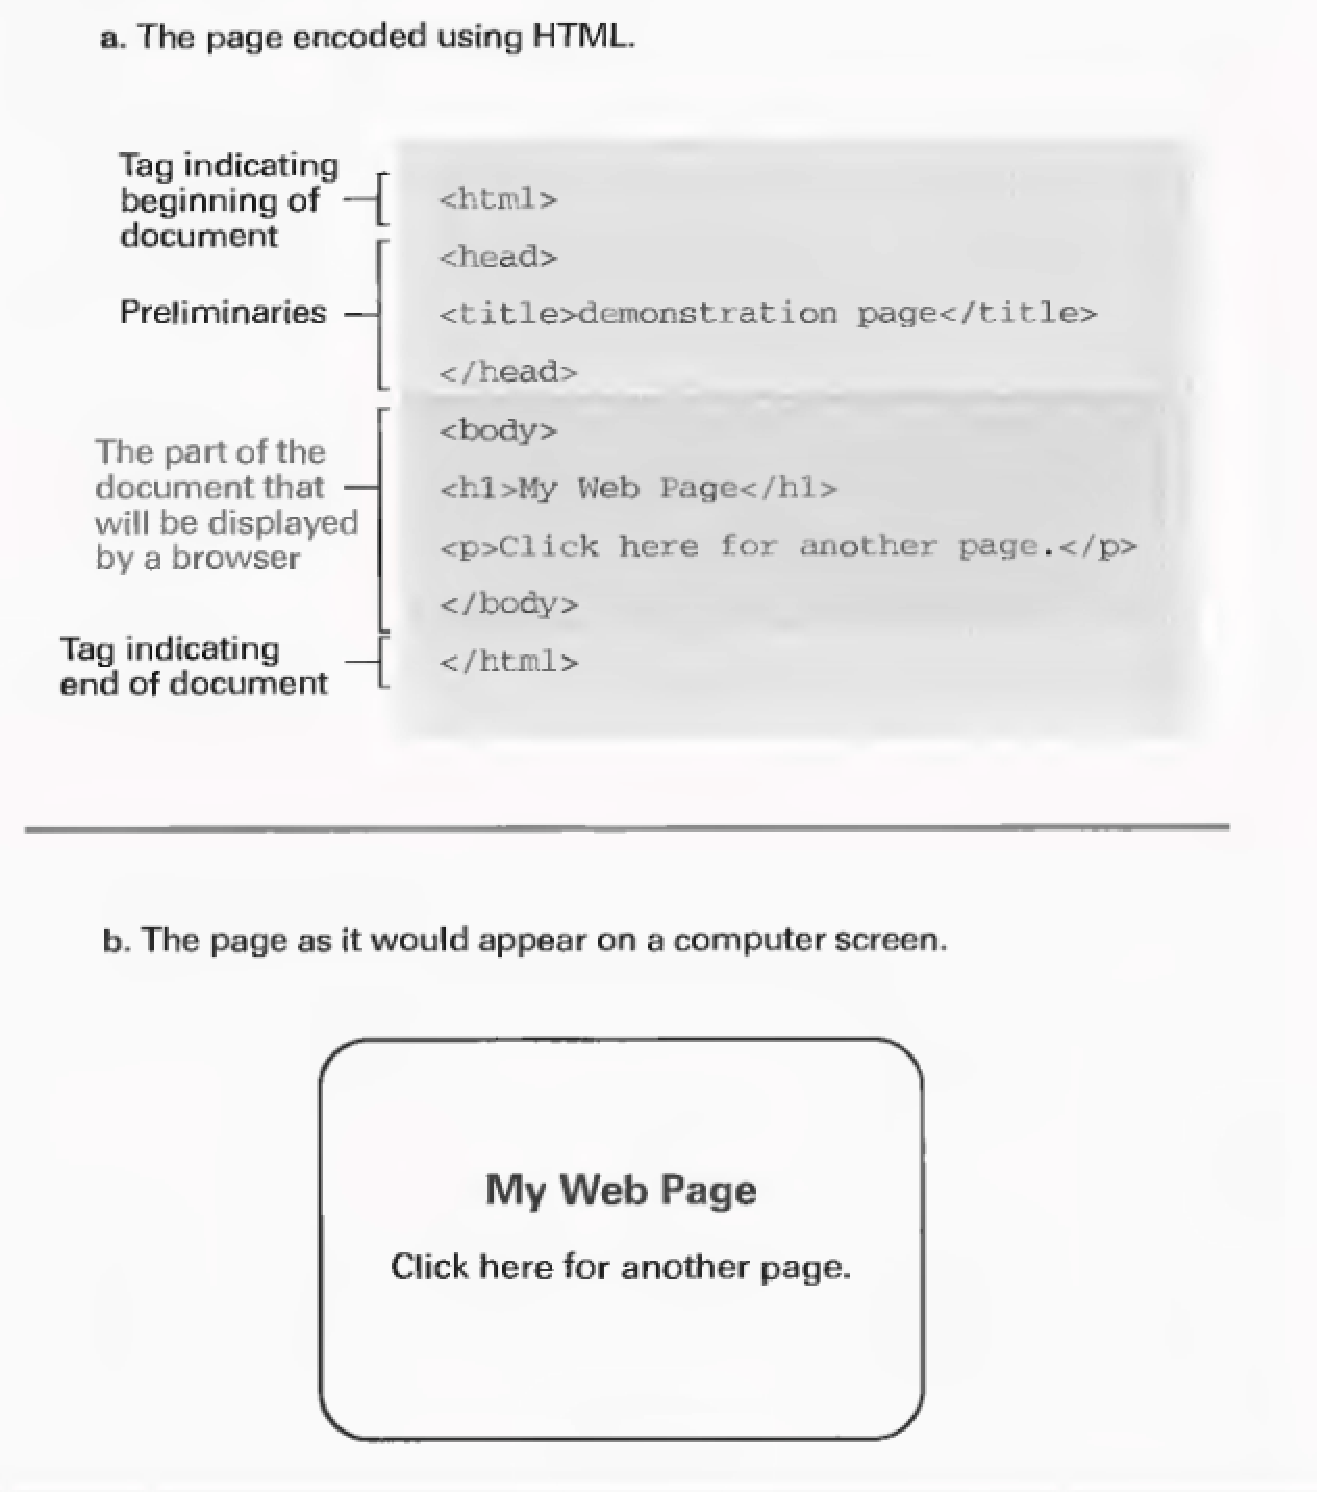
\includegraphics{ch5/fig49.pdf}}
  \caption{Một trang Web đơn giản}
  \label{fig:fig4.9}
\end{figure}

Bản HTML được mã hóa (gọi là bản nguồn) của một trang Web cực kỳ đơn giản được chỉ ra
trong Hình~\ref{fig:fig4.9}a. Cần chú ý rằng các thẻ được phác họa qua các ký tự
\texttt{<} và \texttt{>}.  Tài liệu HTML nguồn bao gồm hai phần--phần đầu (được bao quanh
bởi cặp thẻ \texttt{<head>} và \texttt{</head>}) và phần thân (được bao quanh bởi cặp thẻ
\texttt{<body>} và \texttt{</body>}). Sự khác biệt giữa phần đầu và phần thân của một
trang Web tương tự như phần đầu và phần thân của một cuốn sổ ghi nhớ trong nội bộ một tổ
chức. Trong cả hai trường hợp, phần đầu thường chứa thông tin sơ bộ về tài liệu (ngày,
tiêu đề,… trong trường hợp của sổ ghi nhớ). Phần thân chứa nội dung cốt lõi của tài liệu,
mà trong trường hợp của trang web thì đó là các tài liệu được trình chiếu trên màn hình
máy tính khi trang đó được hiển thị lên.

Phần đầu của trang Web hiển thị trong Hình~\ref{fig:fig4.9}a chứa chỉ duy nhất tiêu đề của
tài liệu (được bao quanh bởi cặp thẻ ``title''). Tiêu đề này chỉ có mang tính chất là dẫn
chứng cho tài liệu; nó không phải là phần được hiển thị lên trên màn hình máy tính. Nội
dung mà sẽ hiển thị lên trên màn hình máy tính được chứa trong phần thân của tài liệu.


Mục đầu tiên trong phần thân của tài liệu trong Hình~\ref{fig:fig4.9}a là tiêu đề cấp độ 1
(được bao quanh bởi cặp thẻ \texttt{<h1>} và \texttt{</h1>}) chứa dòng văn bản ``My Web
Page.''. Là tiêu đề cấp độ 1 có nghĩa là trình duyệt sẽ hiển thị văn bản này nổi bật trên
màn hình. Mục tiếp theo trong phần thân là một đoạn văn bản (được bao quanh bởi cặp thẻ
\texttt{<p>} và \texttt{</p>}) chứa đoạn văn bản ``Click here for another
page.''. Hình~\ref{fig:fig4.9}b chỉ ra trang web sẽ được hiển thị như thế nào trên màn
hình máy tính thông qua một trình duyệt.

Trong hình dạng hiện tại của nó, trang Web trong Hình~\ref{fig:fig4.9} không có đầy đủ các
chức năng nên khi đó sẽ không có gì xảy ra khi người xem kích chuột vào từ \textit{here},
 mặc dù theo yêu cầu trình duyệt sẽ phải hiển thị một trang khác. Để đạt được yêu cầu, ta cần phải liên kết từ \textit{here} tới một tài liệu khác.

\begin{figure}
  \centering \scalebox{0.5}{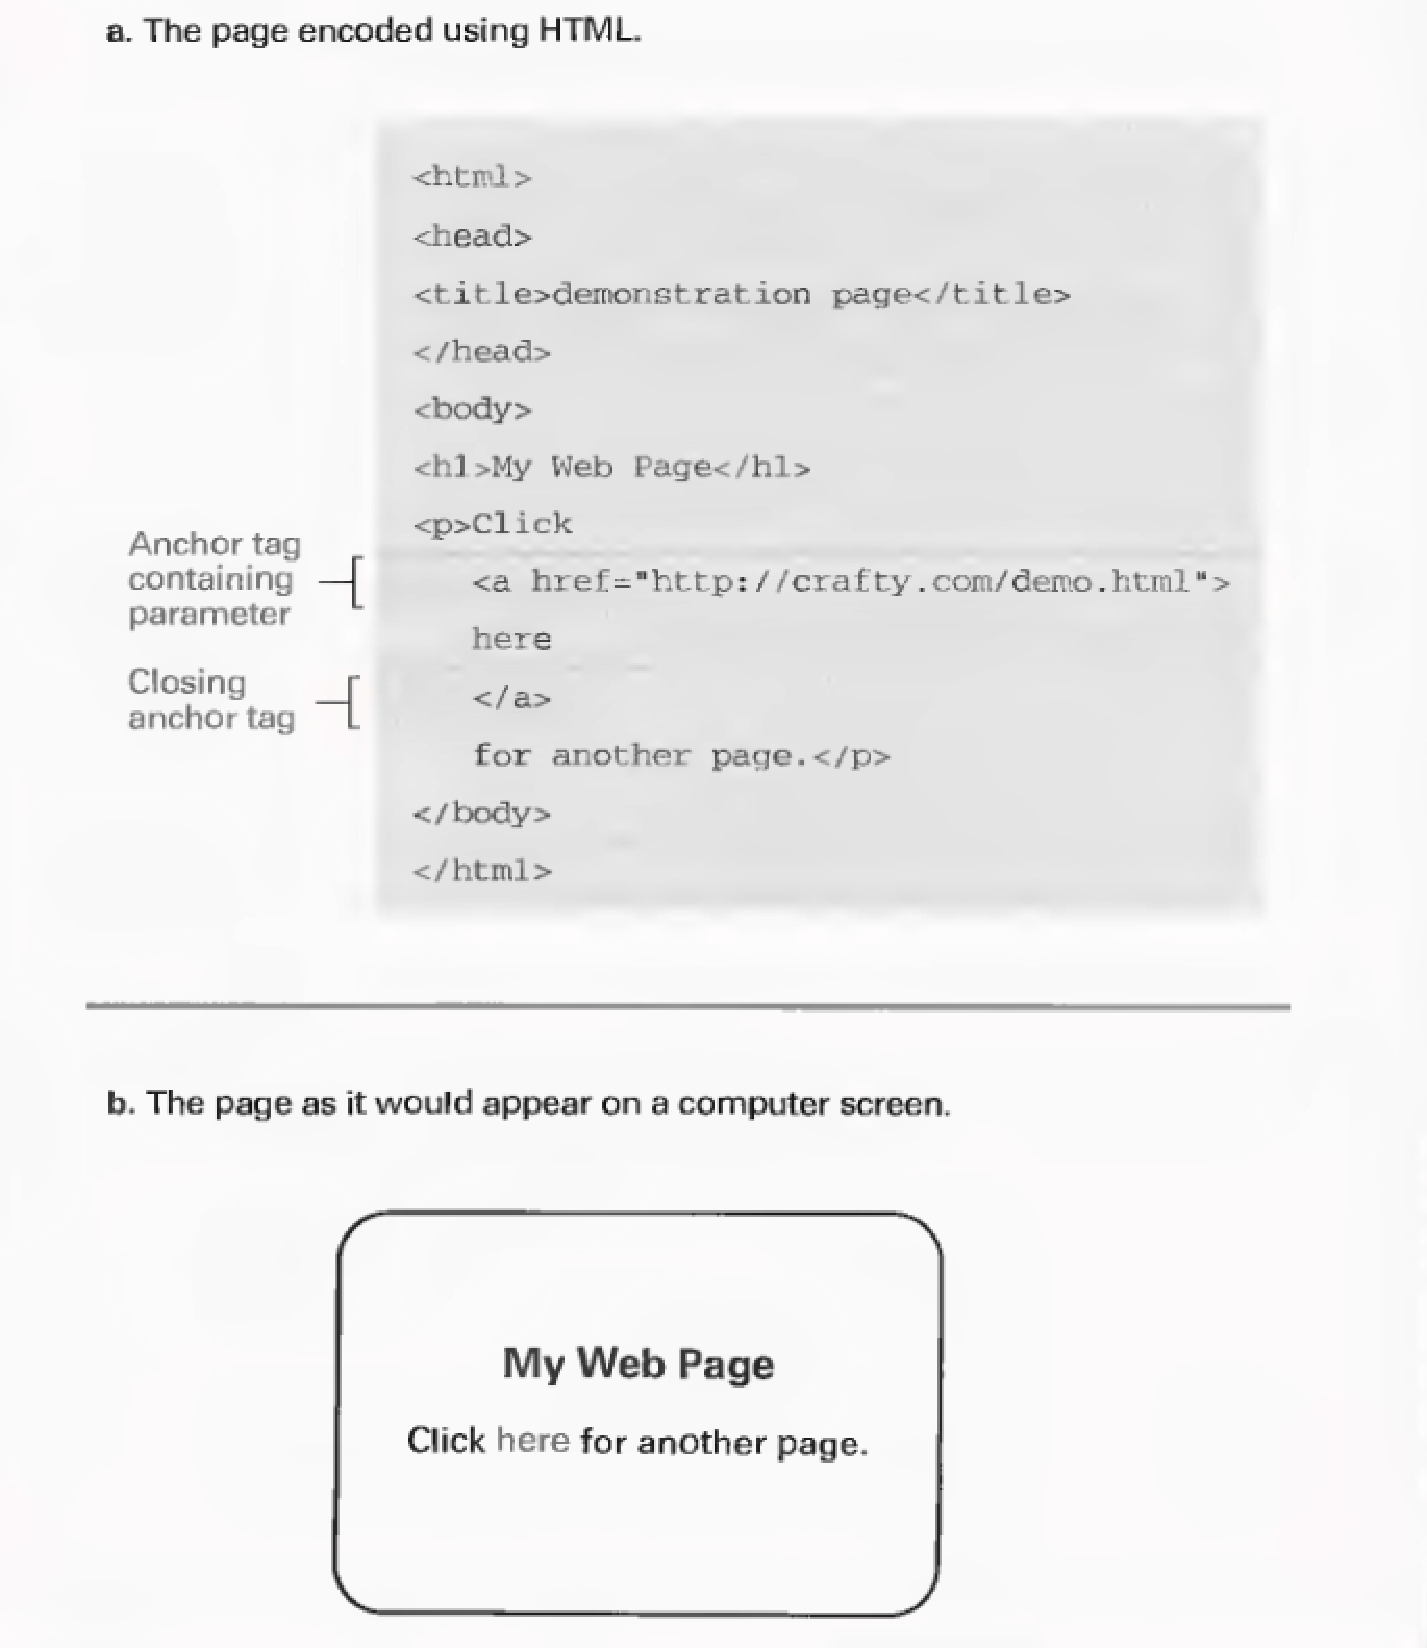
\includegraphics{ch5/fig410.pdf}}
  \caption{Một trang Web mở rộng}
  \label{fig:fig4.10}
\end{figure}

Ta giả sử rằng khi từ here được kích chuột vào, ta muốn trình duyệt truy lục và hiển thị
trang web tại URL \url{http://crafty.com/demo.html}. Để làm được điều đó, trước tiên ta
phải bao quanh từ \texttt{here} trong bản nguồn của trang bằng cặp thẻ \texttt{<a>} và
\texttt{</a>}, cặp thẻ này được gọi là thẻ mấu neo. Bên trong thẻ mở mấu neo, ta chèn thêm
tham số \texttt{href= “http://crafty.com/demo.html”} (như trong Hình~\ref{fig:fig4.10}a)
với mục đích chỉ ra siêu văn bản tham chiếu (href: hypertext reference) kết hợp với thẻ
trong URL ngay sau dấu bằng (\url{http://crafty.com/demo.html})

Khi có thêm các thẻ mấu neo, trang Web bây giờ sẽ hiển thị trên màn hình máy tính như
trong Hình~\ref{fig:fig4.10}b. Chú ý rằng sự hiển thị này tương tự như trong
Hình~\ref{fig:fig4.9}b ngoại trừ từ \textit{here} được làm cho nổi bật bằng mầu sắc, điều
đó chỉ ra rằng nó là một liên kết tới một tài liệu Web khác. Việc kích chuột vào những cụm
từ nổi bật như vậy sẽ khiến cho trình duyệt truy lục và hiển thị tài liệu Web kết hợp
trong liên kết đó. Chính vì vậy thông qua các thẻ mấu neo mà các tài liệu Web được liên
kết tới những tài liệu khác.

Cuối cùng, ta cũng cần phải được nói sơ qua làm thế nào để một hình ảnh có thể được
hiển thị trên một trang Web đơn giản. Với ý định này, giả sử rằng một ảnh mã hóa theo định
dạng JPEG mà ta muốn chèn vào được lưu trữ trong cùng thư mục với bản nguồn HTML của
trang Web trên site chủ HTTP. Ngoài ra, ta cũng giả sử rằng tên của tệp ảnh đó là
\texttt{OurImage.jpg}. Với những điều kiện như vậy, ta có thể ra chỉ thị cho một
trình duyệt hiển thị ảnh đó trên đầu của trang Web bằng cách chèn vào thêm thẻ hình ảnh
(img) \texttt{<img src = "OurImage.jpg">} ngay sau thẻ \texttt{<body>} trong tài liệu
nguồn HTML. Điều này diễn đạt cho trình duyệt hiểu là một ảnh có tên là
\texttt{OurImage.jpg} có thể được hiển thị tại vị trí đầu tiên của tài liệu. (Ký hiệu
\texttt{src} là dạng viết ngắn gọn của từ ``source'', có nghĩa là thông tin đằng sau dấu
bằng chỉ ra đường dẫn tới tệp hình ảnh mà sẽ được hiển thị.) Khi trình duyệt tìm thấy thẻ
này, nó sẽ gửi một thông điệp ngược trở về ứng dụng chủ HTTP mà từ đó, ứng dụng chủ sẽ
nhận được yêu cầu của tài liệu gốc tới tệp hình ảnh \texttt{OurImage.jpg} và sau đó trình
duyệt sẽ hiển thị hình ảnh một cách thích hợp.

Nếu ta di chuyển thẻ hình ảnh tới cuối cùng của tài liệu, ngay trước thẻ
\texttt{</body>}, khi đó trình duyệt sẽ hiển thị hình ảnh tại vị trí cuối cùng của trang
Web. Tất nhiên, có nhiều kỹ thuật phức tạp hơn cho việc đặt vị trí của một hình ảnh trên
một trang Web, nhưng chúng không nhất thiết phải được đề cập tới ở đây.

\subsection*{XML}

HTML về cơ bản là một hệ thống ký hiệu mà qua đó một tài liệu văn bản với việc hiển thị
của tài liệu đó có thể được mã hóa như là một tệp văn bản đơn giản. Theo cách thức tương
tự thì ta cũng có thể mã hóa một tài liệu không còn là nguyên bản như những tệp văn
bản--một ví dụ là về các bản nhạc. Khi lưu trữ thông tin về một mẫu khuông nhạc, các đường
gạch nhịp và nốt trong đó âm nhạc được miêu tả theo cách truyền thống không được thể hiện
theo định dạng từng ký tự một của những tệp văn bản. Tuy nhiên, ta có thể khắc phục
được vấn đề này bằng cách phát triển một hệ thống ký hiệu thay thế. Nói một cách chính xác
hơn, ta có thể thỏa thuận trình bày bắt đầu của khuông nhạc bằng thẻ \texttt{<staff
  clef = ``treble''>}, kết thúc một khuông nhạc bằng thẻ \texttt{</staff>}, trình bày ký
hiệu nhịp theo dạng \texttt{<time> 2/4 </time>}, thẻ bắt đầu và kết thúc của một nhịp là
\texttt{<measure>} và \texttt{</measure>}, và theo một thứ tự định sẵn thì một nốt như nốt
thứ tám trên điệu thứ C được ký hiệu là \texttt{<notes>eight C</notes>},… Khi đó, đoạn văn
bản sau:
\begin{verbatim}
      <staff clef = "treble">
           <key>C minor</key>
           <time> 2/4 </time>
           <measure> 
               <rest> egth </rest> 
               <notes> egth G, egth G, egth G </notes>
           </measure>
           <measure> 
               <notes> hlf E </notes>
           </measure>
      </staff>
\end{verbatim}
có thể được sử dụng để mã hóa bản nhạc chỉ ra trong Hình~\ref{fig:fig4.11}.

\begin{figure}[bt] 
  \centering \scalebox{0.4}{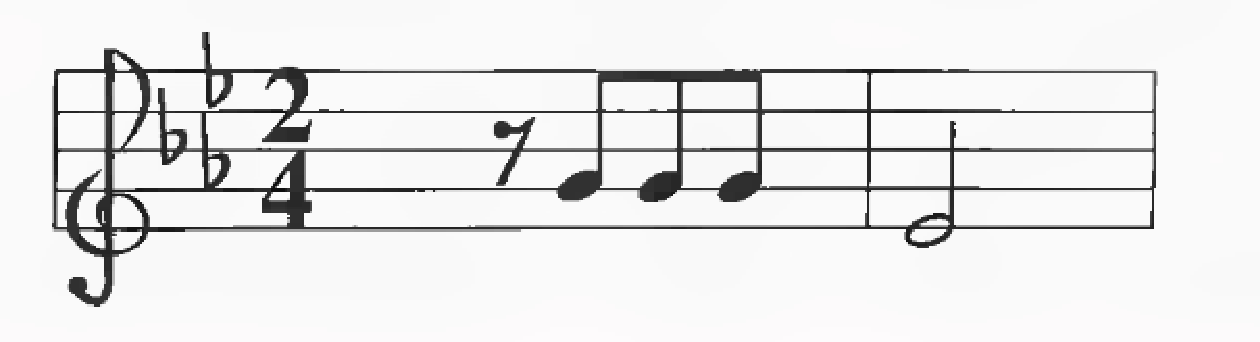
\includegraphics{ch5/fig411.pdf}}
  \caption{Hai khuông đầu tiên trong bản Symphony thứ năm của Beethoven}
  \label{fig:fig4.11}
\end{figure}


Bằng việc sử dụng những ký hiệu như vậy, một bản nhạc có thể được mã hóa, sửa đổi, lưu trữ
và truyền qua mạng Internet như những tệp văn bản. Hơn nữa, phần mềm có thể được viết ra
nhằm trình diễn nội dung của những tệp văn bản như vậy theo một khuôn dạng âm nhạc truyền
thống hay thậm chí có thể chơi được bản nhạc đó trên một nhạc cụ điện tử.

Chú ý rằng hệ thống mã hóa bản nhạc của ta bao gồm khuôn dạng tương tự được sử dụng bởi
ngôn ngữ HTML. Ta đã lựa chọn cách thức ký hiệu những thẻ nhận dạng các thành phần bởi cặp
ký tự \texttt{<} và \texttt{>}. Ta cũng quyết định chỉ ra điểm bắt đầu và kết thúc của
những cấu trúc đó (ví dụ như một khuông nhạc, một chuỗi các nốt nhạc, hay một nhịp nhạc)
bởi những thẻ có tên trùng nhau-–thẻ kết thúc được ký hiệu thêm một ký tự \texttt{/} (thẻ
\texttt{<measure>} được kết thúc bằng thẻ \texttt{</measure>)}. Và ta cũng đã quyết định
chỉ ra những thuộc tính đặc biệt bên trong các thẻ bằng các biểu thức như \texttt{clef =
  “treble”}. Khuôn dạng tương tự này có thể cũng được sử dụng để phát triển các hệ thống
mô tả những định dạng khác như các biểu thức toán học hay đồ họa.

Ngôn ngữ \textbf{đánh dấu mở rộng} (XML: Extensible Markup Language) là một khuôn dạng
được chuẩn hóa (tương tự như ví dụ về bản nhạc của ta) cho việc thiết kế những hệ
thống ký hiệu cho việc hiển thị những dữ liệu dạng như các tệp văn bản. (Trên thực tế, XML
là một ngôn ngữ dẫn xuất được làm đơn giản hóa từ một tập các chuẩn cũ hơn gọi là Standard
Generalized Markup Language, với ký hiệu viết tắt là SGML.)  Theo như chuẩn XML, những hệ
thống ký hiệu với tên gọi là \textbf{ngôn ngữ đánh dấu} được phát triển cho việc mô tả
toán học, trình diễn đa phương tiện, và âm nhạc. Nói tóm lại, HTML là ngôn ngữ đánh dấu
dựa trên chuẩn XML mà được phát triển nhằm hiển thị các trang Web. (Thực tế là phiên bản
gốc của HTML được phát triển trước chuẩn XML đã được làm cho vững chắc, và do đó một vài
tính năng của HTML không thích ứng hoàn toàn với XML. Điều này cũng giải thích vì sao bạn
có thể đã thấy những tham khảo về XHTML, đó là một phiên bản của HTML với một sự kết hợp
khá chặt chẽ với XML.)

XML cung cấp một tiền lệ tốt cho việc làm thế nào mà các chuẩn được thiết kế được ứng dụng
trong phạm vi rộng. Đúng hơn là với những ngôn ngữ đánh dấu không liên quan cho việc mã
hóa rất nhiều dạng tài liệu, việc thiết kế một cách độc đáo phương pháp biểu diễn bằng XML
là nhằm phát triển một chuẩn chung cho các ngôn ngữ đánh dấu khác. Với chuẩn này, những
ngôn ngữ đánh dấu có thể được khai thác trong rất nhiều các ứng dụng. Những ngôn ngữ đánh
dấu được phát triển theo cách thức này đều có một tính chất giống nhau mà cho phép chúng
kết hợp với nhau nhằm thu được những ngôn ngữ đánh dấu dùng cho những ứng dụng phức tạp
như những tài liệu văn bản chứa các phân đoạn của một bản nhạc và các biểu thức toán học.

Cuối cùng ta cũng cần phải chú ý rằng XML công nhận sự phát triển của những ngôn ngữ
đánh dấu mới khác so với HTML mà trong đó chúng có mục đích là làm nổi bật ngữ nghĩa hơn
là việc hiển thị. Ví dụ, với HTML các thành phần (ingredient) trong một công thức làm món
ăn có thể được đánh dấu sao cho chúng xuất hiện như là một danh sách mà trong đó mỗi thành
phần được đặt trên một dòng riêng biệt. Nhưng nếu ta sử dụng các thẻ định hướng có
ngữ nghĩa (semantic-oriented), các thành phần trong công thức đó có thể được đánh dấu dưới
dạng như những thành phần hợp thành tổng quát (có thể chỉ sử dụng các thẻ như
\texttt{<ingredient>} và \texttt{</ingredient>}) hơn là các mục chọn đơn thuần trong một
danh sách. Sự khác biệt ở đây tuy là rất nhỏ nhưng lại khá quan trọng. Cách tiếp cận theo
hướng có ngữ nghĩa sẽ cho phép các công cụ tìm kiếm có thể xác định những công thức món ăn
chứa hay không chứa những thành phần nào đó, đây sẽ là một cải tiến đáng kể vượt qua tình
trạng hiện tại của đề tài nghiên cứu mà trong đó chỉ những công thức chứa hay không chứa
những từ cụ thể mới được xác định. Nói một cách chính xác hơn, nếu các thẻ có ngữ nghĩa
được sử dụng, một công cụ tìm kiếm có thể xác định công thức cho món lasagna không chứa
rau bina (spinach), trong khi đó một cách thức tìm kiếm dựa vào chỉ đơn thuần là nội dung
của từ sẽ bỏ qua một công thức mà bắt đầu bằng câu ``This lasagna does not contain
spinach.'' Tóm lại, bằng việc sử dụng một chuẩn có phạm vi trên mạng Internet cho việc
đánh dấu các tài liệu theo hướng có ngữ nghĩa hơn là việc hiển thị, một Web \textit{ngữ
  nghĩa} phạm vi toàn cầu (World Wide Semantic Web) có thể sẽ được tạo ra thay thế cho Web
cú pháp phạm vi toàn cầu (World Wide Syntactic Web) mà ta đang có hiện nay.

\subsection*{Các hoạt động phía client và phía server}

Bây giờ ta xem xét các bước được yêu cầu đối với một trình duyệt để có thể truy nạp
được trang Web đơn giản đã chỉ ra trong Hình~\ref{fig:fig4.10} và hiển thị nó lên màn hình
máy tính qua trình duyệt. Trước tiên, đóng vai trò của một ứng dụng khách, trình duyệt sẽ
sử dụng thông tin có được trong URL (có thể nhận được từ người sử dụng trình duyệt) để
liên lạc tới ứng dụng phục vụ Web, điều khiển truy cập tới trang Web và yêu cầu một bản
sao của trang Web cần phải được truyền tới ứng dụng khách. Ứng dụng chủ sẽ đáp lại yêu cầu
bằng cách gửi tài liệu văn bản được hiển thị trong Hình~\ref{fig:fig4.10}a đến trình
duyệt. Trình duyệt sau đó sẽ dịch các thẻ HTML có trong tài liệu nhằm xác định trang Web
đó cần được hiển thị như thế nào và trình diễn tài liệu đó trên màn hình máy tính của
trình duyệt một cách phù hợp. Người sử dụng trình duyệt sẽ nhìn thấy một hình ảnh như được
mô tả trong Hình~\ref{fig:fig4.10}b. Nếu người dùng sau đó kích chuột vào từ
\textit{here}, trình duyệt sẽ sử dụng URL trong thẻ mấu neo kết hợp trong đó để liên lạc
tới ứng dụng chủ tương ứng nhằm thu nạp và hiển thị một trang Web khác. Nói tóm lại, quá
trình này bao gồm chỉ đơn thuần là thao tác lấy và hiển thị các trang Web một cách trực
tiếp bởi người dùng.

Nhưng nếu ta muốn một trang Web trong đó bao gồm cả hoạt ảnh (animation) hay một
trang Web cho phép khách hàng điền đầy đủ những thông tin vào một đơn đặt hàng và gửi đơn
đặt hàng đó đi? Những thứ đó cần phải yêu cầu hoạt động bổ trợ từ trình duyệt hay ứng dụng
phục vụ Web. Những hoạt động như vậy được gọi là những hoạt động \textbf{phía client}
(client-side) nếu chúng được thực hiện bởi một ứng dụng khách (ví dụ như một trình duyệt)
hay \textbf{phía server} (server-side) nếu chúng được thực hiện bởi một ứng dụng phục vụ
(ví dụ như ứng dụng phục vụ Web).

Hoạt ảnh trên một trang Web thông thường là một hoạt động phía client. Thông tin cần có
cho hoạt ảnh được truyền tới trình duyệt cùng với văn bản có trong trang Web. Sau đó hoạt
ảnh mới được thực thi dưới sự điều khiển của trình duyệt.

Ngược lại, giả sử một đại lý du lịch yêu cầu các khách hàng cần phải xác định đích đến
mong muốn và ngày du lịch, khi đó đại lý sẽ trình chiếu cho khách hàng một trang Web đã
được tùy biến chỉ chứa thông tin thích hợp với nhu cầu của khách hàng. Trong trường hợp
này, website của đại lý du lịch trước tiên sẽ cung cấp một trang Web và được hiển thị cho
một khách hàng với những đích đến có thể. Dựa trên những thông tin cơ bản này, khách hàng
sẽ chỉ ra những đích đến yêu thích và những ngày du lịch mà họ mong muốn (một hoạt động
phía client). Thông tin này sau đó sẽ được truyền về ứng dụng chủ của đại lý nơi mà nó sẽ
được dùng để tạo dựng một trang Web tương ứng đã được tùy biến (một hoạt động phía server)
và sau đó sẽ được gửi tới trình duyệt của khách hàng.

Một ví dụ tương tự xảy ra trong trường hợp một người sử dụng những dịch vụ của một công cụ
tìm kiếm. Ở đây, người này chỉ ra một chủ đề ưa thích (một hoạt động phía client) mà sau
đó được truyền tới công cụ tìm kiếm, nơi mà một trang Web được tùy biến xác định những tài
liệu nào có thể phù hợp được tạo dựng (một hoạt động phía server) và gửi trả về cho ứng
dụng khách.

Có rất nhiều hệ thống thực hiện các hoạt động phía client và phía server, mỗi hệ thống đều
cạnh tranh với hệ thống khác bằng những tính năng nổi bật của mình. Có một cách thức điều
khiển các hoạt động phía client tuy đã ra đời từ sớm những vẫn khá phổ biến, đó là việc
triển khai viết các chương trình dưới mã của ngôn ngữ Javascript (được phát triển bởi Công
ty truyền thông Netscape) bên trong tài liệu nguồn HTML của một trang Web. Khi đó, một
trình duyệt có thể bóc tách những chương trình này và thực hiện chúng theo đúng yêu
cầu. Một cách tiếp cận khác (được phát triển bởi Sun Microsystems) là trước tiên truyền
một trang Web tới trình duyệt và sau đó truyền những đơn vị chương trình bổ trợ gọi là
applet (được viết bằng ngôn ngữ Java) tới trình duyệt theo yêu cầu bên trong tài liệu
nguồn HTML. Vẫn còn một cách tiếp cận khác nữa đó là hệ thống Flash (được phát triển bởi
Macromedia), thông qua hệ thống Flash, những trình diễn đa phương tiện trên diện rộng có
thể được triển khai một cách đơn giản.


Một cách thức điều khiển các hoạt động phía server là sử dụng một tập các chuẩn gọi là CGI
(Common Gateway Interface) mà qua đó các ứng dụng khách có thể yêu cầu thực thi các chương
trình được lưu trữ trên một máy chủ. Một biến tố của cách tiếp cận này (được phát triển
bởi Sun Microsystems) là cho phép các ứng dụng khách khiến  những đơn vị chương trình
như servlet được thực thi trên phía ứng dụng chủ. Một phiên bản được đơn giản hóa của cách
tiếp cận servlet có thể được sử dụng khi yêu cầu được gửi tới phía server là việc tạo dựng
một trang Web được tùy biến, như trong ví dụ về đại lý du lịch. Trong trường hợp này, các
mẫu trang Web được gọi là JavaServer Pages (JSP) được lưu trữ tại máy chủ phục vụ Web và
được bổ sung từ những thông tin nhận từ phía một ứng dụng khách nào đó. Một cách tiếp cận
tương tự được sử dụng bởi Microsoft, nơi mà các mẫu từ những trang Web được tùy biến được
tạo dựng ra với tên gọi là Active Server Page (ASP). Ngược lại với những hệ thống đòi hỏi
cần phải có bản quyền, PHP (tiền thân xuất phát từ Personal Home Page nhưng ngày nay được
hiểu với nghĩa mới là PHP Hypertext Processor) là một hệ thống mã nguồn mở cũng rất thích hợp cho việc triển
khai các tính năng phía server.

Cuối cùng, sẽ thật là thiếu sót nếu ta không nhận ra những vấn đề về an ninh và 
quy tắc phát sinh từ việc cho phép những ứng dụng khách và ứng dụng phục vụ thực hiện những
chương trình trên máy tính của người khác. Trên thực thế những ứng dụng phục vụ Web đó
thường truyền tải các chương trình tới phía các ứng dụng khách nơi mà chúng được thực thi
dẫn tới những sự nghi ngờ liên quan đến vấn đề về nội quy trên phía ứng dụng chủ và những
vấn đề về bảo mật trên phía ứng dụng khách. Nếu ứng dụng khách thực thi bất kỳ chương
trình nào một cách mù quáng được gửi tới từ một ứng dụng phục vụ Web, nó có thể mở cửa
chính mình cho các hoạt động nguy hiểm được thực hiện bởi ứng dụng chủ. Tương tự như vậy,
trên thực tế những ứng dụng khách này có thể là nguyên nhân khiến cho các chương trình có
thể được thực thi trên ứng dụng chủ dẫn tới những vấn đề về nội quy trên phía ứng dụng
khách và những vấn đề liên quan đến bảo mật trên phía ứng dụng chủ. Nếu một ứng dụng chủ
nào đó thực hiện một cách mù quáng bất kỳ chương trình nào được gửi tới mình từ một ứng
dụng khách bất kỳ, những lỗ hổng an ninh và sự thiệt hại tiềm năng trên máy chủ có thể sẽ
xảy ra.

\subsection*{Câu hỏi \& Bài tập}

\begin{enumerate}
\item Một URL là gì? Một trình duyệt là gì?
\item Một ngôn ngữ đánh dấu là gì?
\item Sự khác nhau giữa HTML và XML là gì?
\item Mục đích của những thẻ HTML dưới đây là gì?

  \begin{inparaenum}[a.]
  \item \texttt{<html>} \qquad
  \item \texttt{<head>} \qquad
  \item \texttt{</body>} \qquad
  \item \texttt{<fa>}
  \end{inparaenum}

\item Những cụm từ phía client (client-side) và phía server (server-side) đề cập tới vấn
  đề gì?
\end{enumerate}






























%%% Local Variables: 
%%% mode: latex
%%% TeX-master: "../tindaicuong"
%%% End: 


\section{Phần đọc thêm: Các giao thức Internet}
\label{sec:4.4}
Trong phần này ta sẽ khám phá những thông điệp được truyền qua mạng Internet như thế
nào. Quá trình truyền này yêu cầu sự cộng tác của tất cả các máy tính trên hệ thống, và do
đó phần mềm điều khiển quá trình này cần phải đặt trên mọi máy tính trên mạng
Internet. Ta bắt đầu nghiên cứu cấu trúc toàn diện của phần mềm này.

\subsection*{Cách tiếp cận theo lớp tới các phần mềm trên mạng Internet}

Một nhiệm vụ chính của phần mềm mạng là cung cấp cơ sở hạ tầng cho việc truyền tải các
thông điệp từ một máy tính này đến một máy tính khác. Trên mạng Internet, hoạt động truyền
thông điệp được hoàn thành dựa trên phân cấp của các đơn vị phần mềm. Việc này tương tự
như bạn gửi một gói quà từ vùng West Coast ở Mỹ tới vùng East Coast ở Mỹ
(Hình~\ref{fig:fig4.12}). Trước hết, bạn sẽ thực hiện bọc quà lại thành một gói và viết
lên gói đó địa chỉ thích hợp. Sau đó, bạn sẽ gửi gói quà này tới một công ty vận chuyển
như U.S. Postal Service. Công ty vận chuyển có thể đặt gói quà đó cùng với những thứ khác
trong một công-ten-nơ và gửi nó tới một hãng hàng không mà các dịch vụ của nó đã được đăng
ký từ trước. Hãng hàng không này đặt công ten nơ trên một máy bay và chuyển tới thành phố
đích, hãng hàng không sẽ gỡ bỏ công ten nơ đó xuống từ máy bay chuyên chở của mình và giao
nó cho một công ty vận chuyển nhằm chuyển tới đích. Tiếp đó, công ty vận chuyển sẽ gỡ gói
hàng của bạn ra khỏi công ten nơ và giao nó tới địa chỉ.

\begin{figure} [tbh]
  \centering \scalebox{0.35}{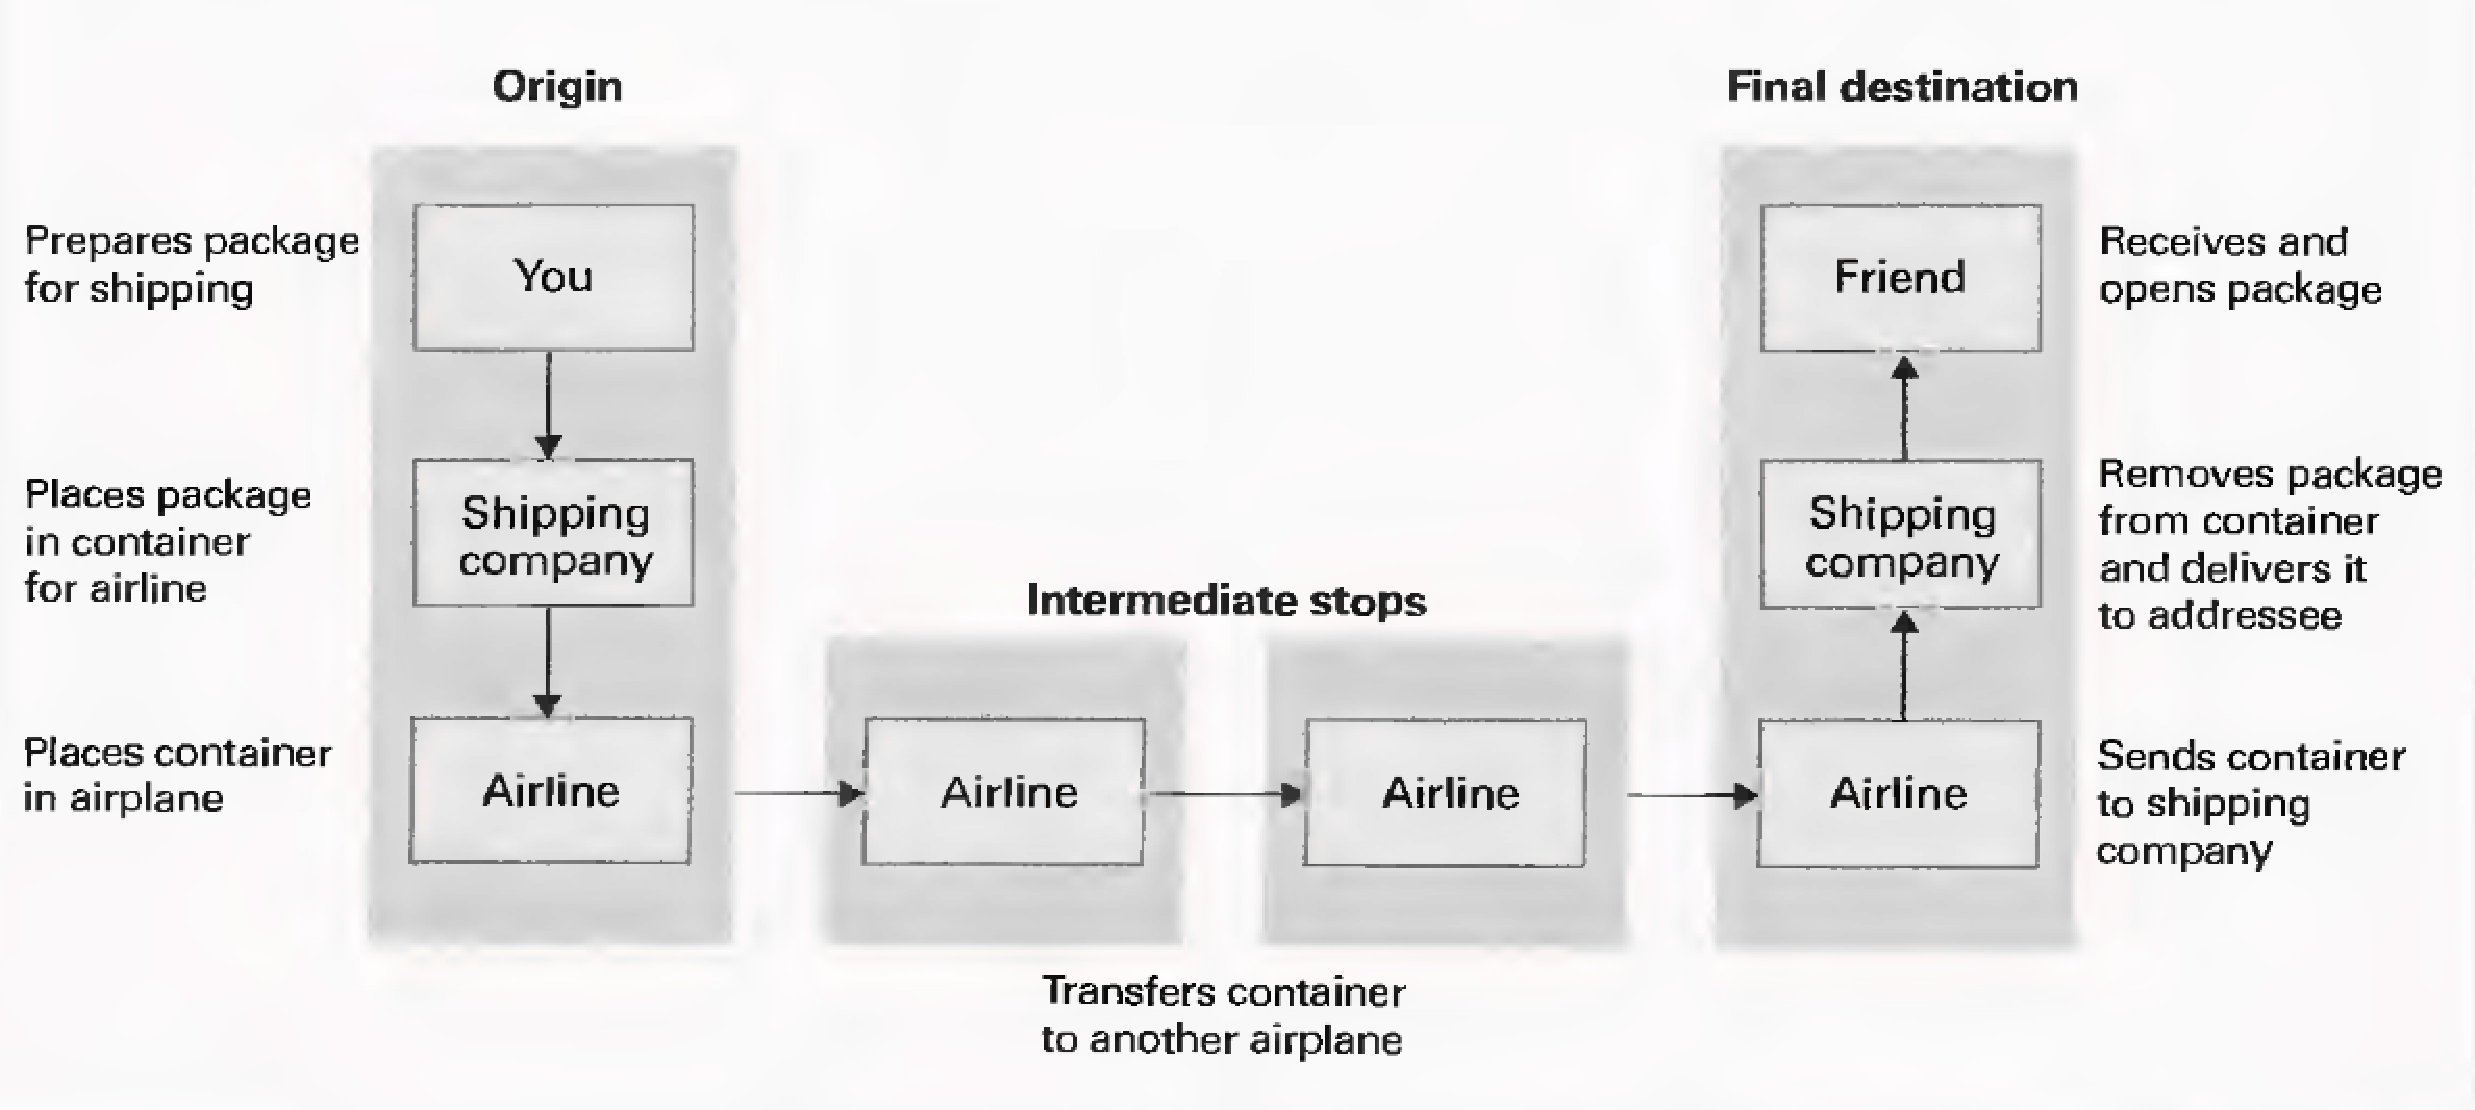
\includegraphics{ch5/fig412.pdf}}
  \caption{Ví dụ việc chuyển gói hàng hoá}
  \label{fig:fig4.12}
\end{figure}

Nói tóm lại, quá trình chuyên chở của gói hàng sẽ được thực hiện theo dạng cây ba cấp
(tầng):
\begin{inparaenum}[(a)]
\item cấp người sử dụng (bao gồm bạn và bạn bè của bạn),
\item công ty vận chuyển, và
\item hãng hàng không.
\end{inparaenum}
Mỗi cấp sử dụng cấp thấp hơn như là một công cụ trừu tượng. (Bạn không cần quan tâm tới
những chi tiết của công ty vận chuyển, và công ty vận chuyển cũng không cần quan tấm tới
những điều hành cục bộ của hãng hàng không.) Mỗi cấp độ trong cây ba cấp đều có những đại
diện ở cả nơi gửi và nơi nhận hàng,.

\begin{figure}[tbh]
  \centering \scalebox{0.35}{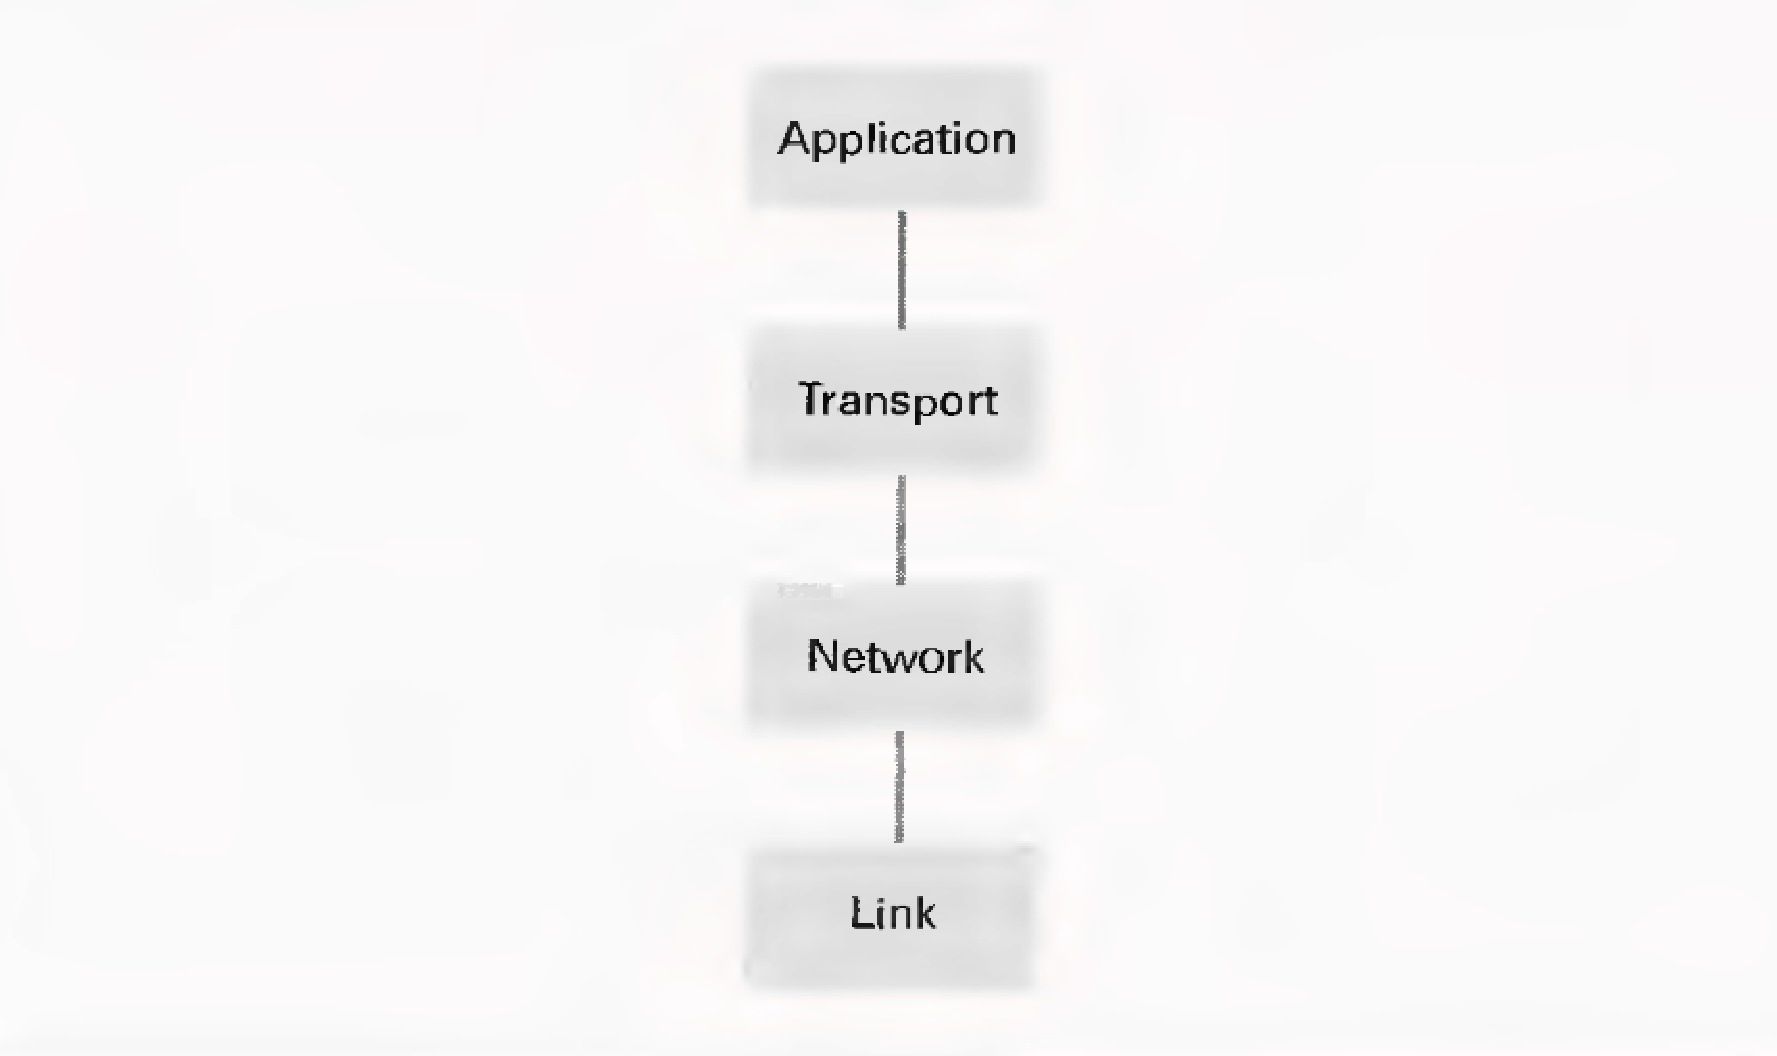
\includegraphics{ch5/fig413.pdf}}
  \caption{Các tầng phần mềm Internet}
  \label{fig:fig4.13}
\end{figure}

Ví dụ như trường hợp với sản phẩm điều khiển truyền thông qua mạng Internet, trừ phần mềm
Internet có bốn tầng chứ không phải ba tầng, thì mỗi phần mềm bao gồm một tập các chương
trình con đúng hơn là con người và công việc kinh doanh. Bốn tầng (cấp) này được biết đến
là \textbf{tầng ứng dụng}, \textbf{tầng vận chuyển}, \textbf{tầng mạng} và \textbf{tầng
  liên kết} (Hình~\ref{fig:fig4.13}). Tất cả các tầng đều hiện diện trên mỗi máy tính trên
mạng Internet. Một thông điệp thông thường đều bắt nguồn từ tầng ứng dụng. Từ đó nó được
chuyển qua xuống tầng vận chuyển và tầng mạng để chuẩn bị cho việc truyền tải, và cuối
cùng nó được truyền đi bởi tầng liên kết. Thông điệp đó được nhận bởi tầng liên kết phía
bên đích và được chuyển lên tầng trên cho đến khi nó được giao cho tầng ứng dụng tại đích
nhận của thông điệp.

Ta hãy xem xét quá trình này một cách kỹ lưỡng hơn bằng cách lần theo vết của một
thông điệp khi nó tìm đường qua hệ thống (Hình~\ref{fig:fig4.14}). Ta bắt đầu quá
trình lần vết tại tầng ứng dụng.


Tầng ứng dụng bao gồm các đơn vị phần mềm như phần mềm khách và phần mềm chủ mà sử dụng
truyền thông Internet để thực hiện những nhiệm vụ của chúng. Mặc dù tên của chúng là giống
nhau, tầng này không bị hạn chế các phần mềm theo sự phân loại ứng dụng được giới thiệu
trong Mục~\ref{sec:3.2}, nhưng cũng bao gồm nhiều gói tiện ích. Ví dụ, phần mềm truyền tải tệp sử
dụng giao thức truyền tệp (FTP) hay phần mềm cung cấp khả năng truy cập từ xa sử dụng
telnet trở nên phổ biến đến nỗi mà chúng thông thường được xem như là phần mềm tiện ích.


\begin{figure} 
  \centering \scalebox{0.5}{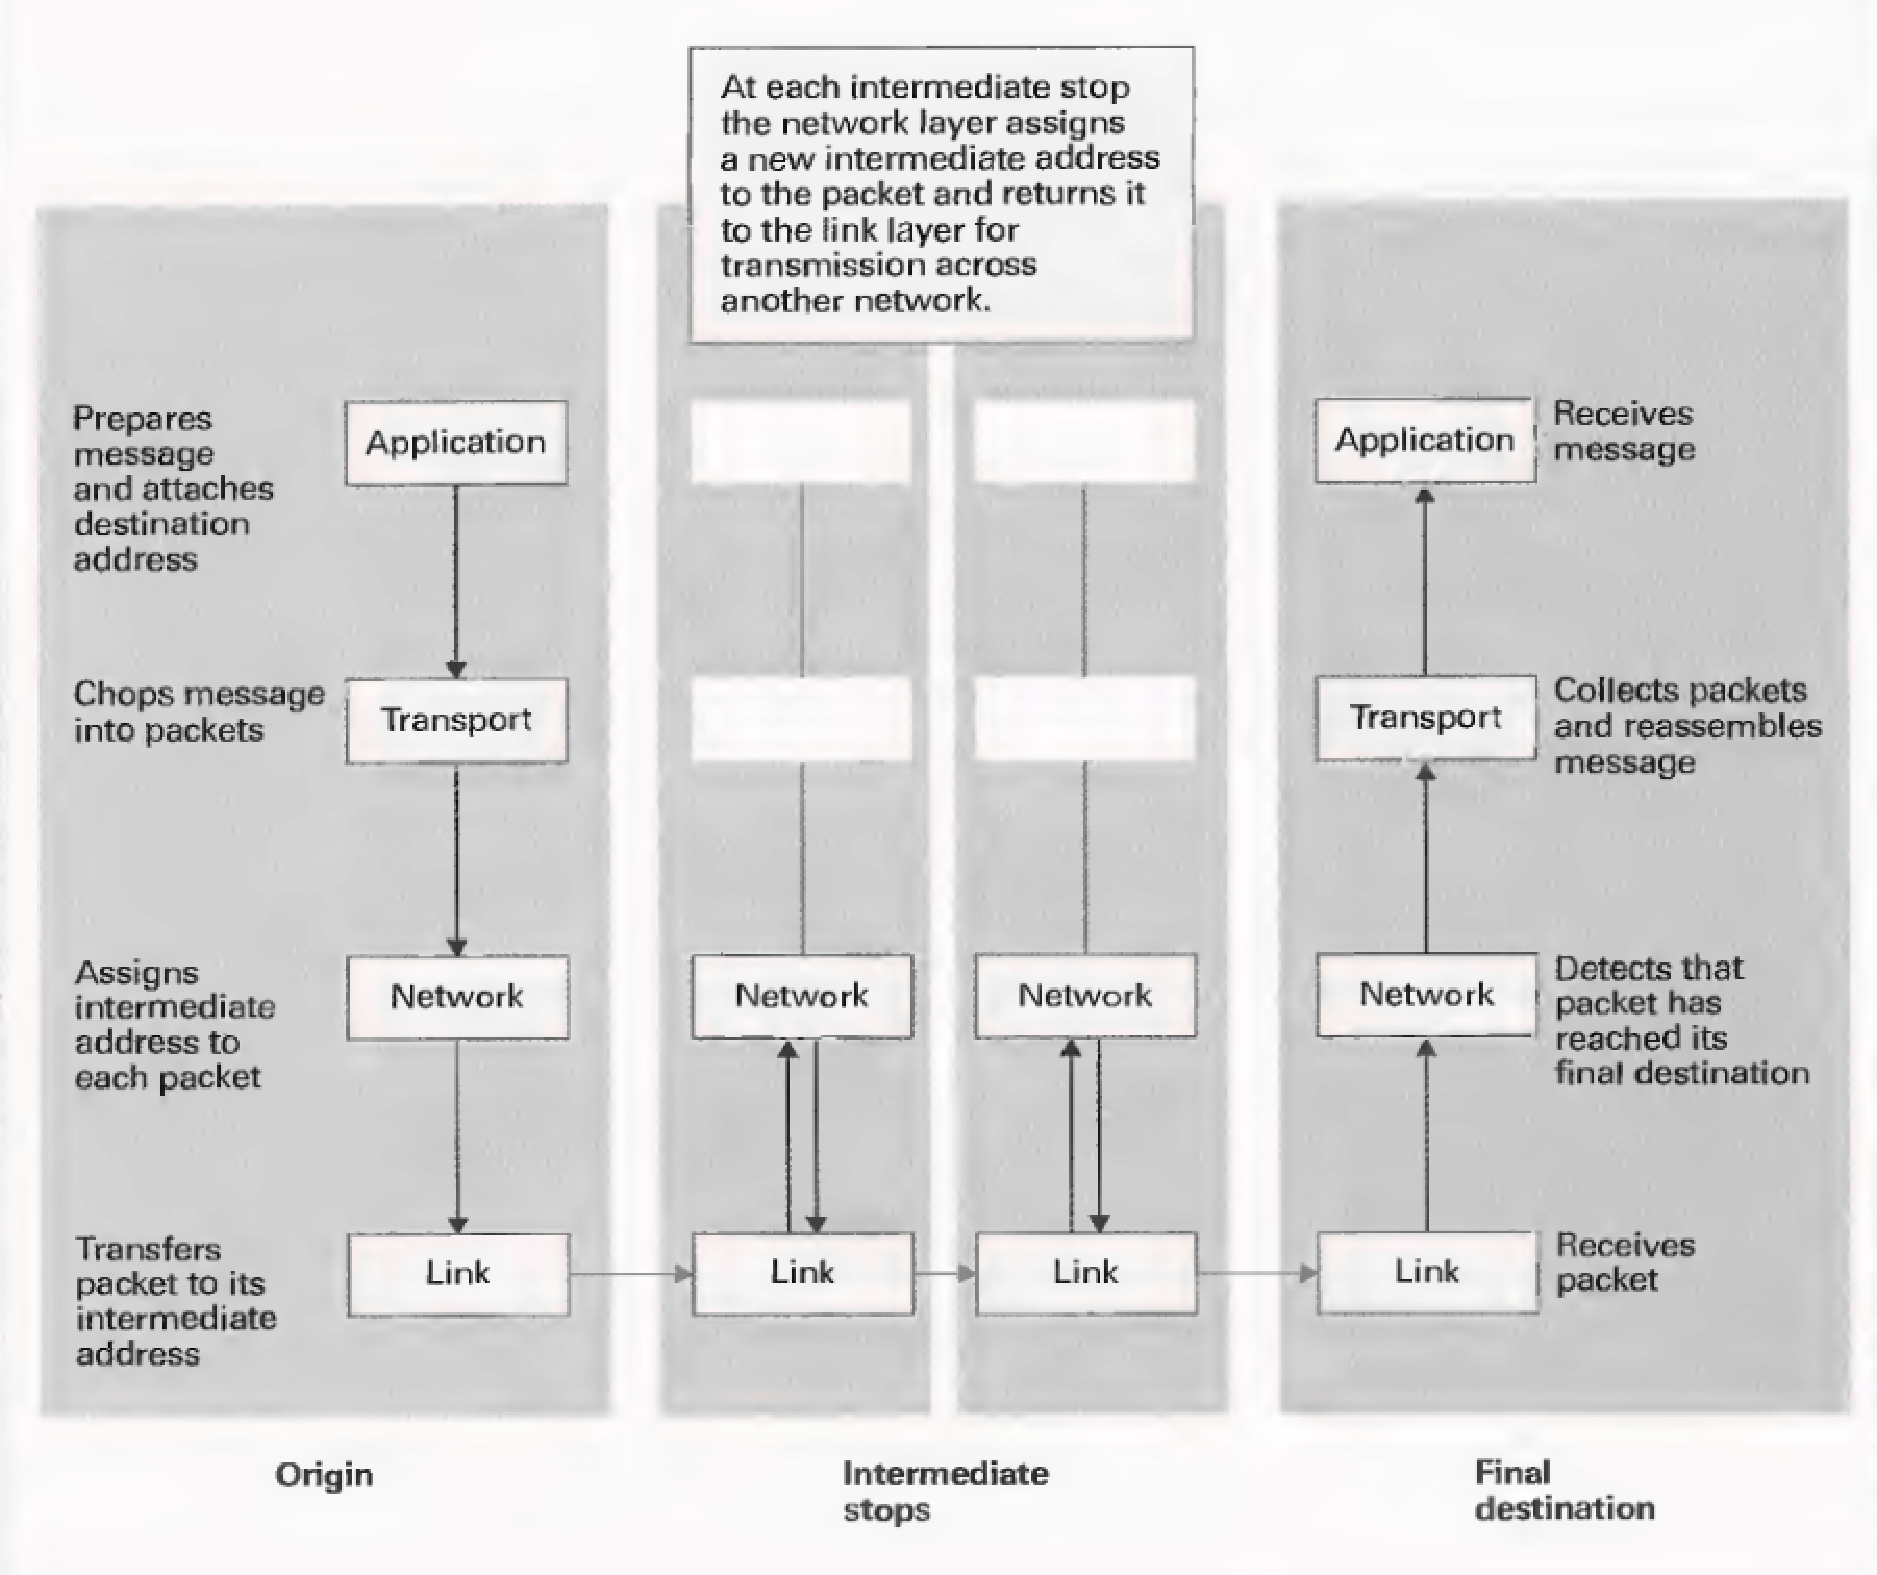
\includegraphics{ch5/fig414.pdf}}
  \caption{Truyền một thông điệp qua Internet}
  \label{fig:fig4.14}
\end{figure}


Tầng ứng dụng sử dụng tầng vận chuyển để gửi và nhận thông điệp qua Internet theo cùng một
cách thức mà ta sử dụng một công ty vận chuyển để gửi và nhận các gói hàng. Tương tự
như trách nhiệm của bạn là phải cung cấp một địa chỉ chi tiết hợp lệ với công ty vận
chuyển, trách nhiệm của tầng ứng dụng cũng là cung cấp một địa chỉ hợp lệ cho tầng vận
chuyển. (Để thực hiện được yêu cầu này, tầng ứng dụng có thể sử dụng các dịch vụ tên miền
trên Internet để chuyển đổi từ địa chỉ dễ nhớ được sử dụng bởi người dùng sang địa chỉ IP
tương thích với mạng Internet.)

Nhiệm vụ chính của tầng vận chuyển là chấp nhận các thông điệp đến từ tầng ứng dụng và đảm
bảo rằng những thông điệp này là đúng định dạng cho việc truyền tải qua mạng Internet. Để
phục vụ cho mục đích sau đó, tầng vận chuyển chia các thông điệp dài thành những đoạn nhỏ
(segment), mà sẽ được truyền qua mạng Internet như những đơn vị độc lập nhau. Việc chia
nhỏ này là cần thiết vì một thông điệp đơn và dài có thể làm tắc nghẽn luồng đi của những
thông điệp khác tại những điểm nút trên mạng Internet nơi mà rất nhiều thông điệp phải
được truyền qua những đoạn đường giao nhau.

Thật vậy, những đoạn thông điệp nhỏ có thể truyền xen lẫn với nhau tại những điểm nút thay vì một thông điệp dài bắt ép những thông điệp khác phải chờ trong khi nó truyền qua (giống
như những chiếc ô tô con phải chờ một đoàn tầu dài đi qua tại một ngã tư đường sắt).

Tầng vận chuyển thêm những số theo một trình tự vào những đoạn thông điệp nhỏ để các đoạn
này có thể được ghép nối lại tại đích của thông điệp. Sau đó nó gắn thêm địa chỉ đích vào
mỗi đoạn thông điệp và chuyển giao những đoạn thông điệp được đánh địa chỉ này, được biết
đến như là các gói tin (packet), cho tầng mạng. Từ đó, các gói tin được xử lý như những
thông điệp riêng rẽ và không liên quan đến nhau cho đến khi chúng được truyền tới tầng vận
chuyển tại đích cuối cùng của chúng.

Có thể nói là các gói tin gắn liền với một thông điệp chung có khả năng đi theo những
đường khác nhau qua mạng Internet.

Tầng mạng có nhiệm vụ là chuyển tiếp những gói tin nó nhận được từ một mạng trên Internet
tới một mạng khác trong quá trình chúng được chuyển tới đích cuối cùng của chúng. Theo
cách đó thì tầng mạng phải làm việc với mô hình của mạng Internet. Nói một cách cụ thể,
nếu đường đi của một gói tin qua mạng Internet phải được truyền qua rất nhiều mạng riêng
lẻ, nó chính là tầng mạng tại mỗi điểm dừng trung gian mà xác định hướng đi  gói tin sẽ
được gửi đi sau đó. Việt quyết định đưa ra ở đây là như sau: Nếu đích cuối cùng của gói
tin là thuộc bên trong của mạng hiện thời, tầng mạng sẽ gửi gói tin đến ngay đó; ngược
lại, tầng mạng sẽ gửi gói tin tới một thiết bị dẫn đường (router) trong mạng hiện tại,
thiết bị dẫn đường này sẽ có nhiệm vụ chuyển tiếp gói tin đến mạng gần kề. Theo cách thức
này thì một gói tin được gửi tới đích là một máy tính trong mạng hiện tại sẽ được gửi ngay
tới máy tính đó, ngược lại thì một gói tin được gửi tới một máy tính nằm ngoài mạng hiện
tại sẽ tiếp tục hành trình của nó từ mạng này sang mạng tiếp theo gần kề cho đến mạng đích
cuối cùng.

Để quyết định đích tiếp theo trong hành trình của gói tin, tầng mạng cập nhật thêm địa chỉ
này vào gói tin như là một địa chỉ trung gian và chuyển giao gói tin này xuống tầng liên
kết.

Tầng liên kết có trách nhiệm truyền tải gói tin tới địa chỉ trung gian mà đã được xác định
bởi tầng mạng ở trên. Do đó, tầng liên kết phải thỏa thuận với sự truyền thông tới mạng
riêng biệt của máy tính. Nếu mạng đó là mạng vòng tròn có sử dụng thẻ bài, tầng liên kết
phải đợi có quyền chiếm hữu thẻ bài trước khi truyền gói tin đi. Nếu mạng sử dụng CSMA/CD,
tầng liên kết phải lắng nghe khi đường trục truyền rỗi mới được thực hiện truyền tải.

Khi một gói tin được truyền đi, nó được nhận bởi tầng liên kết tại máy tính được chỉ định
rõ bởi địa chỉ cục bộ đã được gắn thêm vào thông điệp. Tại đó, tầng liên kết sẽ chuyển
giao gói tin lên tầng mạng, nơi mà đích cuối cùng của gói tin được so sánh và kiểm tra với
địa chỉ hiện tại. Nếu những địa chỉ này không trùng khớp, tầng mạng xác định một địa chỉ
trung gian mới cho gói tin, đính kèm địa chỉ đó vào gói tin và đưa gói tin quay trở về
tầng liên kết để tiếp tục thực hiện truyền gói tin đi. Trong cách thức này, mỗi gói tin
được chuyển qua từng máy tính trên hành trình tới đích của nó. Cần chú ý rằng chỉ có tầng
liên kết và tầng mạng mới liên quan tại những điểm dừng trung gian trong suốt hành trình
này (xem lại Hình~\ref{fig:fig4.14}).

Nếu tầng mạng xác định rằng một gói tin đến đã tiến tới được đích cuối cùng, nó sẽ chuyển
giao gói tin đó cho tầng vận chuyển. Khi tầng vận chuyển nhận được các gói tin được gửi
tới từ tầng mạng, nó sẽ bóc tách những thông tin cần thiết bên trong của những đoạn tin và
xây dựng lại thông điệp gốc ban đầu dựa trên những số trình tự mà đã được cung cấp bởi
tầng vận chuyển tại nơi gửi của thông điệp. Khi thông điệp được ghép nối lại, tầng vận
chuyển thực hiện chuyển giao nó cho đơn vị phần mềm thích hợp trên tầng ứng dụng--kết thúc
quá trình truyền thông của thông điệp.


Việc xác định xem đơn vị phần mềm nào trong tầng ứng dụng được phép nhận một thông điệp
được gửi tới là nhiệm vụ quan trọng của tầng vận chuyển. Nhiệm vụ này được thực hiện thông
qua việc gán những \textbf{số cổng} duy nhất (không liên quan đến những cổng I/O đã được
thảo luận trong Chương~\ref{chap:2}) cho các đơn vị phần mềm khác nhau và yêu cầu số cổng thích
hợp được chèn thêm vào địa chỉ của thông điệp trước khi bắt đầu gửi thông điệp. Sau đó,
khi thông điệp được nhận bởi tầng vận chuyển tại đích nhận, tầng vận chuyển chỉ đơn thuần
chuyển giao thông điệp đó cho phần mềm trên tầng ứng dụng có cổng được chỉ định trước.

Người sử dụng của mạng Internet rất hiếm khi cần phải quan tâm tới những con số cổng này
bởi vì những ứng dụng thông thường thường có những cổng đã được công nhận một cách phổ
biến. Ví dụ, nếu một trình duyệt Web được yêu cầu tải một tài liệu mà URL của nó là
\url{http://www.zoo.org/animals/frog.html}, trình duyệt sẽ thừa nhận rằng nó cần phải liên
lạc với một phần mềm chủ HTTP tại địa chỉ \url{www.zoo.org} thông qua cổng 80. Tương tự
như vậy, khi truyền tải một tệp, một phần mềm khách FTP cũng thừa nhận rằng nó cần phải
giao tiếp với phần mềm chủ FTP thông qua cổng~20 và 21.

Nói tóm lại, việc truyền thông qua mạng Internet bao gồm sự tương tác giữa bốn tầng của
phần mềm. Tầng ứng dụng xử lý các thông điệp đứng trên góc độ tầm nhìn của ứng dụng. Tầng
vận chuyển chuyển đổi những thông điệp này thành những gói tin mà tương thích với mạng
Internet và tập hợp những thông điệp mà nhận được trước khi giao chúng cho ứng dụng thích
hợp. Tầng mạng liên quan đến việc gửi trực tiếp những gói tin qua mạng Internet. Tầng liên
kết đảm nhận việc truyền thông thực sự của những gói tin từ máy tính này tới máy tính
khác. Với tất cả các hoạt động này, có thể nói là hết sức kinh ngạc với thời gian trả lời
của mạng Internet được đo lường theo đơn vị phần nghìn giây (millisecond) thì rất nhiều
giao dịch xuất hiện ngay tức thời.

\subsection*{Bộ giao thức TCP/IP}

Yêu cầu đặt ra cho các hệ thống mạng mở đã phát sinh một nhu cầu cho những chuẩn được
công bố bởi các hãng sản xuất có thể cung cấp thiết bị và phần mềm mà hoạt động một cách
đúng đắn với những sản phẩm của các hãng khác. Một chuẩn mà kết quả là mô hình tham chiếu
Hệ thống mở kết nối liên mạng (OSI: Open System Interconnection), đã được đưa ra bởi Tổ
chức quốc tế về tiêu chuẩn hóa (International Organization Standardization). Chuẩn này
được dựa trên một hệ thống phân cấp bảy tầng trái với hệ thống phân cấp bốn tầng mà chúng
ta đã xem xét ở trên. Nó là một mô hình often-quoted vì nó mang theo uy quyền của một tổ
chức quốc tế, nhưng nó cũng làm trì hoãn việc thay thế quan điểm về mô hình bốn tầng, chủ
yếu là bởi vì nó được thiết lập sau hệ thống phân cấp bốn tầng vốn đã trở thành một chuẩn
trên thực tế cho mạng Internet.


Bộ giao thức TCP/IP là một tập các giao thức được sử dụng bởi mạng Internet nhằm triển
khai việc liên lạc theo hệ thống phân cấp trên mạng Internet. Trên thực tế, \textbf{Giao
  thức Điều khiển Việc truyền tải(TCP)} (TCP: Transmission Control Protocol) và
\textbf{Giao thức Mạng Internet (IP)} (IP: Internet Protocol) là tên của chỉ hai trong số
những giao thức trong tập giao thức rộng lớn này--thực tế là toàn bộ tập hợp này được hiểu
như là bộ giao thức TCP/IP. Một cách chính xác hơn, TCP định nghĩa một phiên bản của tầng
vận chuyển. Ta phát biểu là một phiên bản bởi vì bộ giao thức TCP/IP cung cấp hơn
một cách thức thực thi tại tầng vận chuyển; một phiên bản khác được định nghĩa bởi giao
thức UDP (User Datagram Protocol). Việc tách đôi như vậy cũng tương tự như trên thực tế
khi việc vận chuyển một gói hàng, bạn có một lựa chọn giữa nhiều công ty vận chuyển, mỗi
công ty lại đưa ra dịch vụ cơ bản là giống nhau nhưng cũng vẫn có những nét đặc trưng duy
nhất cho từng công ty. Do phụ thuộc vào chất lượng đặc biệt của dịch vụ đã yêu cầu, một
đơn vị trên tầng ứng dụng có thể lựa chọn gửi dữ liệu đi thông qua một trong hai phiên bản
của tầng vận chuyển, TCP hoặc UDP (Hình~\ref{fig:fig4.15})

\begin{figure} [tbh]
  \centering \scalebox{0.5}{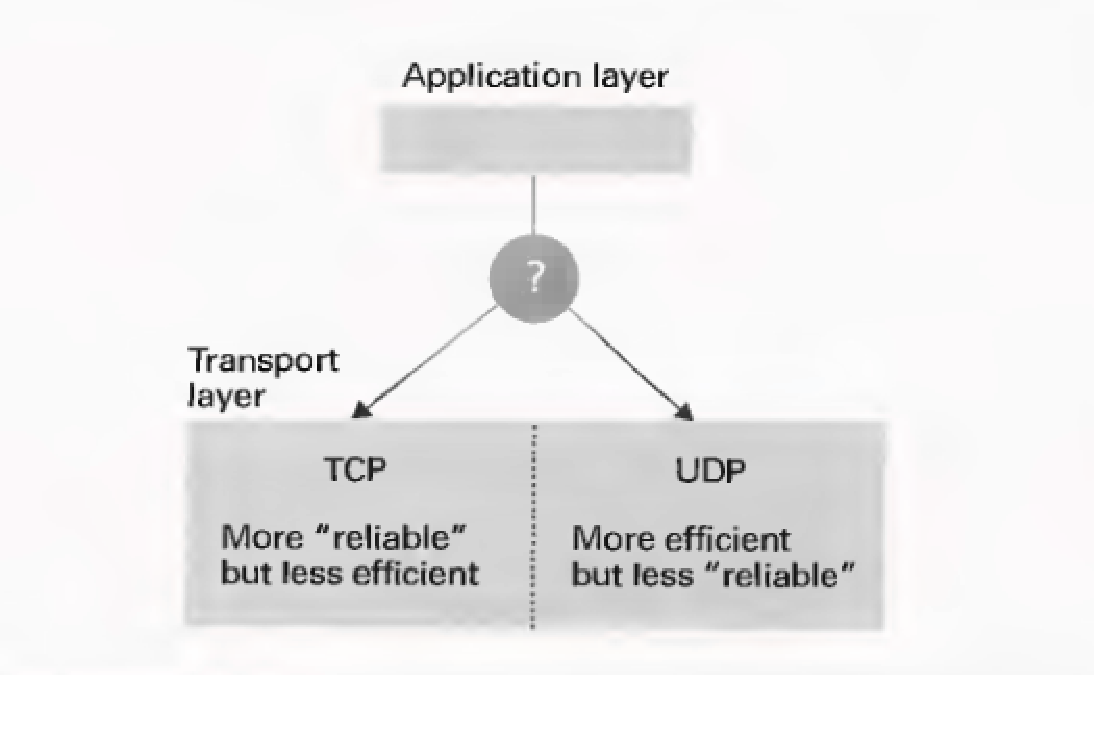
\includegraphics{ch5/fig415.pdf}}
  \caption{Lựa chọn giữa TCP và UDP}
  \label{fig:fig4.15}
\end{figure}


Có hai điểm khác biệt cơ bản giữa TCP và UDP. Thứ nhất là trước khi gửi một thông điệp
được yêu cầu bởi tầng ứng dụng, tầng vận chuyển sử dụng giao thức TCP để gửi thông điệp
của chính nó tới tầng vận chuyển của bên đích nói rằng một thông điệp sắp được gửi sang
đó. Sau đó nó sẽ chờ thông điệp này được công nhận trước khi bắt đầu gửi thông điệp của
tầng ứng dụng. Theo cách đó, tầng vận chuyển sử dụng giao thức TCP sẽ thiết lập một kết
nối trước khi gửi một thông điệp. Còn tầng vận chuyển sử dụng giao thức UDP không thiết
lập một kết nối như vậy trước khi gửi một thông điệp. Tầng vận chuyển chỉ đơn thuần gửi
thông điệp nào đó tới địa chỉ mà nó nhận được và không quan tâm đến địa chỉ đó. Với tất cả
những gì mà nó biết được, máy tính đích có thể không sẵn sàng hoạt động. Với lý do này,
UDP được gọi là giao thức không có kết nối.

Sự khác biệt cơ bản thứ hai giữa TCP và UDP là tầng vận chuyển sử dụng giao thức TCP tại
nguồn gửi và đích nhận là cùng làm việc với nhau theo cách thức trả lời xác nhận và truyền
lại gói tin nhằm chắc chắn rằng tất cả các đoạn tin của thông điệp thực sự đã được truyền
tới đích thành công. TCP được gọi là giao thức tin cậy, trong khi đó thì UDP do không đưa
ra dịch vụ truyền lại nên được gọi là giao thức không tin cậy. Điều này không có nghĩa là
UDP là một lựa chọn tồi. Sau tất cả những điều trên, ta có thể kết luận tầng vận
chuyển sử dụng giao thức UDP được tổ chức hợp lý hơn so với tầng vận chuyển sử dụng giao
thức TCP, và do đó nếu một ứng dụng được chuẩn bị để có thể đạt được những kết quả tiềm
tàng của UDP, ý kiến đó có thể sẽ là một sự lựa chọn tốt hơn. Ví dụ, thư điện tử (email)
thông thường được gửi thông qua giao thức TCP nhưng sự truyền tải thực hiện thông qua hệ
thống máy chủ tên miền khi chuyển đổi những địa chỉ từ dạng dễ nhớ sang dạng IP lại sử
dụng giao thức UDP.

IP là một chuẩn của mạng Internet đối với tầng mạng. Một trong số những đặc tính của nó là
mỗi khoảng thời gian tầng mạng sử dụng giao thức IP lại chuẩn bị một gói tin để gửi xuống
tầng liên kết, nó sẽ thêm một giá trị được gọi là bộ đếm bước truyền, hay thời gian sống
(time to live), vào gói tin đó. Giá trị này là một giới hạn cho số lần gói tin được chuyển
tiếp khi nó cố thử tìm một đường đi qua mạng Internet. Mỗi khoảng thời gian tầng mạng sử
dụng giao thức IP chuyển tiếp một gói tin, nó sẽ giảm bộ đếm bước truyền xuống một giá
trị. Với thông tin này, tầng mạng có thể bảo vệ cho mạng Internet bởi sự lặp vòng vô hạn
của các gói tin trong hệ thống. Cho dù mạng Internet vẫn tiếp tục phát triển từ những thời
sơ khai của nó, một bộ đếm bước truyền ban đầu với giá trị là 64 là chưa đủ để cho phép
một gói tin có thể tìm được đường đi của nó khi được truyền xuyên suốt qua mê cung của
những mạng LAN, MAN, WAN, và các bộ dẫn đường.

Cho đến nay một phiên bản của giao thức IP được biết đến là IPv4 (IP phiên bản 4) đã được
sử dụng trong việc thực thi tầng mạng trong mạng Internet. Tuy nhiên, mạng Internet đã
nhanh chóng phát triển và vượt ra ngoài phạm vi hệ thống 32 bít địa chỉ của IPv4. Do đó,
một phiên bản mới của giao thức IP được biết đến là Ipv6, sử dụng địa chỉ liên mạng bao
gồm 128 bít, đã được thiết lập. Quá trình chuyển đổi từ IPv4 sang IPv6 hiện nay vẫn đang
thực hiện. (Đây là sự chuyển đổi mà ta đã được xem xét qua phần giới thiệu về địa
chỉ Internet trong Mục~\ref{sec:4.2}) Trong một vài phạm vi, IPv6 đang được sử dụng trên thực tế;
một vài phạm vi khác, sự chuyển đổi vẫn đang tiếp diễn trong một vài năm nữa. Ví dụ, theo
những kế hoạch hiện tại của chính phủ Hoa Kỳ là chuyển đổi sang IPv6 trước năm 2008. Trong
bất kỳ trường hợp nào, địa chỉ 32 bít trên mạng Internet vẫn được mong đợi là sẽ không còn
được sử dụng trước năm 2025.

\subsection*{Câu hỏi \& Bài tập}

\begin{enumerate}
\item Những tầng nào trong hệ thống phân cấp của phần mềm Internet được sử dụng để chuyển
  tiếp một thông điệp đến sang một máy tính khác?

\item Chỉ ra một vài sự khác biệt giữa tầng vận chuyển sử dụng giao thức TCP và tầng vận
  chuyển sử dụng giao thức UDP?

\item Làm thế nào để phần mềm Internet có thể đảm bảo rằng các thông điệp không bị chuyển
  tiếp trên mạng Internet mãi mãi?

\item Điều gì khiến cho một máy tính trên mạng Internet tránh được thao tác ghi lại các
  bản sao của những thông điệp truyền qua nó?

\end{enumerate}


%%% Local Variables: 
%%% mode: latex
%%% TeX-master: "../tindaicuong"
%%% End: 

\section{An toàn và bảo mật}
\label{sec:4.5}
Khi một máy tính được kết nối vào một hệ thống mạng, nó trở thành một chủ thể cho sự truy
cập bất hợp pháp và những hành động cố ý phá hoại. Trong phần này ta bàn về những
chủ đề liên quan đến vấn đề này.

\subsection*{Các dạng tấn công}

Có rất nhiều cách thức mà một hệ thống máy tính và nội dung bên trong nó có thể bị tấn
công thông qua những kết nối mạng. Rất nhiều trong số đó kết hợp với nhau chặt chẽ qua
việc sử dụng những \textbf{phần mềm độc hại} (gọi chung là malware). Những phần mềm như
vậy có thể được truyền tới, hay thực hiện trên chính máy tính chứa nó, hay nó có thể tấn
công máy tính từ một điểm cách xa. Những ví dụ của phần mềm là nó được truyền tới, và thực
hiện trên những máy tính thông qua các dạng tấn công bao gồm vi rút (virus), sâu máy tính
(worm), con ngựa thành Troa (Trojan horse), và phần mềm gián điệp (spyware), tên của chúng
phản ánh đặc tính tiêu biểu của phần mềm.

\textbf{Vi rút} là một phần mềm tiêm nhiễm vào một máy tính thông qua việc chèn thêm chính
nó vào các chương trình có sẵn trên máy tính đó. Sau đó, khi chương trình ``chủ'' được
thực thi, vi rút đó cũng được thực thi. Khi được thực thi, nhiều vi rút thực hiện một công
việc là cố gắng lây nhiễm chính bản thân chúng sang các chương trình khác trên máy
tính. Tuy nhiên, một vài vi rút thực hiện những hành động tàn phá như là làm hỏng một vài
tính năng của hệ điều hành, xóa những khối dữ liệu lớn trên bộ nhớ thứ cấp, hay làm sai
lệch dữ liệu và các chương trình khác.

\textbf{Sâu máy tính} là một chương trình tự trị mà tự động truyền nó qua một mạng máy
tính, thường trú trên các máy tính và chuyển tiếp các bản sao của chính nó sang các máy
tính khác. Cũng tương tự như trường hợp của vi rút, một sâu máy tính có thể được thiết kế
đơn thuần là tạo bản sao chính nó hay thực hiện một vài hành động phá phách mang tính nguy
hại. Một đặc tính hệ quả của sâu máy tính là sự phát triển mạnh mẽ của các bản sao sâu máy
tính làm suy biến việc thực thi của các ứng dụng hợp pháp và có thể làm cho một hệ thống
mạng hay một hệ thống liên mạng bị quá tải thực sự.

\textbf{Con ngựa thành Troa} là một phần mềm mà xâm nhập vào một hệ thống máy tính và cải
trang như là một chương trình được người dùng mong đợi, như là một trò chơi hay một gói
ứng dụng có ích, nó được nạp một cách tự nguyện bởi chính nạn nhân. Tuy nhiên, khi đã ở
trong máy tính, con ngựa thành Troa thực hiện thêm những hành động mà có thể tạo ra những
hậu quả nguy hại. Đôi khi những hành động thêm vào đó bắt đầu được thực hiện ngay lập
tức. Trong một số trường hợp, con ngựa thành Troa có thể nằm im lìm cho đến khi được kích
hoạt thông qua một sự kiện đặc biệt như sự kiện của một ngày định trước nào đó. Con ngựa
thành Troa thường đến dưới dạng là những tệp đính kèm vào những thông điệp thư điện tử hấp
dẫn, lôi cuốn người dùng. Khi tệp đính kèm được mở ra (nghĩa là khi người nhận yêu cầu xem
tệp đính kèm), những hành vi xấu xa của con ngựa thành Troa được kích hoạt. Do đó, ta
không nên mở những tệp đính kèm thư điện tử từ những nguồn không quen biết.

Một dạng khác của những phần mềm độc hại là \textbf{phần mềm gián điệp} (đôi khi còn được
gọi là \textbf{sniffing} software), là một phần mềm mà thực hiện thu thập thông tin về
những hoạt động tại máy tính mà nó thường trú và thông báo những thông tin đó về kẻ chủ
mưu của cuộc tấn công. Một vài công ty sử dụng phần mềm gián điệp như là một cách thức để
xây dựng được bộ thông tin về các khách hàng của mình, và trong trường hợp này, vẫn còn có
những nghi ngờ về phẩm chất đạo đức của họ. Trong những trường hợp khác, những phần mềm
gián điệp được sử dụng cho những mục đích hiểm độc một cách hiển nhiên như là ghi lại
những chuỗi ký tự được gõ tại bàn phím của máy tính nhằm tìm ra được mật khẩu hay số thẻ
tín dụng của người dùng.


Ngược lại với việc thu thập thông tin một cách bí mật bằng cách sniffing thông qua phần
mềm gián điệp, \textbf{phishing} là một kỹ thuật thu thập thông tin một cách rõ ràng qua
việc xin phép một cách đơn giản. Cách thức của \textit{phishing} là lợi dụng kỹ thuật moi
từ khi tiến trình liên quan được tung ra dưới dạng vô số ``tuyến'' với hy vọng một ai đó
sẽ ``bị mắc bẫy''. Phishing thường được thực hiện thông qua thư điện tử, và theo dạng này,
nó thường nhỏ gọn hơn kiểu lừa đảo cổ bằng điện thoại. Thủ phạm gửi các thông điệp thư
điện tử giả dạng dưới sự giám sát của một tổ chức tài chính, một văn phòng chính phủ, hay
có lẽ một cơ quan thi hành luật nào đó. Bức thư điện tử yêu cầu nạn nhân tiềm năng của nó
cung cấp thông tin mà được cho rằng là cần thiết cho những mục đích hợp pháp. Tuy nhiên,
thông tin thu được đó lại được sử dụng bởi chính thủ phạm phát tán thư điện tử trong những
mục đích thù địch.

Trái ngược với sự tổn thất từ những lây nhiễm cục bộ bởi vi rút và phần mềm gián điệp, một
máy tính trong một mạng có thể cũng bị tấn công bởi một phần mềm được thực hiện trên các
máy tính khác trong cùng hệ thống. Một ví dụ là \textbf{tấn công từ chối dịch vụ}, là dạng
mà một máy tính bị quá tải khi phải xử lý những yêu cầu liên tiếp. Những kiểu tấn công từ
chối dịch vụ đã bắt đầu chống lại những phần mềm phục vụ Web thương mại trên mạng Internet
nhằm đánh sập sự kinh doanh của một công ty và trong một số trường hợp có thể khiến cho
các hoạt động thương mại của công ty bị đình trệ.

Một kiểu tấn công từ chối dịch vụ đòi hỏi phát sinh một số lượng lớn các yêu cầu trong một
khoảng thời gian ngắn. Để làm được điều đó, kẻ tấn công thường gài một phần mềm trên một
số lượng lớn các máy tính không bị nghi ngờ mà từ các máy tính này sẽ phát sinh các yêu
cầu khi nhận được một tín hiệu điều khiển. Sau đó, khi tín hiệu điều khiển được đưa ra,
tất cả các máy tính này sẽ làm máy phục vụ đích bị ngập lụt bởi các thông điệp.

Như vậy, tính vốn có trong các kiểu tấn công từ chối dịch vụ chính là tính sẵn sàng sử
dụng của những máy tính không bị nghi ngờ được sử dụng như là những kẻ tòng phạm. Điều này
cũng giải thích vì sao tất cả những người sử dụng máy tính cá nhân (PC users: Personal
Computer users) được khuyến cáo là nên ngắt kết nối máy tính của mình tới mạng Internet
khi không sử dụng đến. Người ta đã ước lượng là từ khi một PC được kết nối tới mạng
Internet, ít nhất một kẻ xâm phạm nào đó sẽ cố gắng khai thác sự tồn tại của nó trong vòng
20 phút. Tóm lại, một PC không được bảo vệ có thể là mối đe dọa đáng kể tới tính toàn vẹn
của mạng Internet.

Một vấn đề khác liên quan đến một số lượng lớn các thông điệp không mong đợi là sự gia
tăng nhanh của thư rác, được gọi là \textbf{spam}. Tự nhiên, không giống như kiểu tấn công
từ chối dịch vụ, một khối lượng lớn spam ít có khả năng làm ngập lụt một hệ thống máy
tính. Thay vào đó, hậu quả của spam là khiến cho chính người nhận được spam bị ngập lụt
trong đống thư rác. Vấn đề này có thể sẽ trở nên tồi tệ hơn bởi trên thực tế, như ta
đã được giới thiệu, spam là môi trường được thông qua một cách rộng rãi giúp cho phishing
và những con ngựa thành Troa có thể làm cho máy tính bị lây nhiễm bởi vi rút và những
chương trình có hại khác.

\subsection*{Phòng chống và chữa trị}

Câu châm ngôn cổ ``Phòng bệnh còn hơn chữa bệnh'' là hoàn toàn đúng trong bối cảnh của sự
kiểm soát bởi hành động cố ý phá hoại qua những kết nối mạng. Một kỹ thuật ngăn chặn chính
là lọc giao thông truyền qua một điểm nút trên mạng, thường thông qua một chương trình gọi
là \textbf{bức tường lửa} (firewall). Ví dụ, một bức tường lửa có thể được cài đặt tại
cổng vào/ra (gateway) của một vùng nhằm lọc các thông điệp truyền vào hay ra khỏi vùng
đó. Những bức tường lửa như vậy có thể được thiết kế nhằm chặn những thông điệp đi ra với
những địa chỉ đích được chỉ định hay nhằm chặn những thông điệp đi vào từ những đích được
biết đến như là những nguồn có vấn đề. Chức năng sau này trở thành một công cụ giúp cho
việc chấm dứt một cuộc tấn công từ chối dịch vụ từ khi nó cung cấp một cách thức chặn
luồng giao thông từ những máy tính tấn công. Một vai trò phổ biến khác của bức tường lửa
tại cổng vào/ra của vùng là chặn tất cả các thông điệp đi vào mà trong đó có những địa chỉ
nguồn thuộc mạng của vùng từ đó một thông điệp như vậy sẽ chỉ ra rằng một máy trạm ngoài
vùng đang giả mạo là một thành viên trong vùng. Việc giả mạo như là một đối tác khác chứ
không phải là chính mình được biết đến với tên gọi là \textbf{spoofing}.


Những bức tường lửa cũng được sử dụng để bảo vệ các máy tính cá nhân hơn là toàn bộ hệ
thống mạng hay vùng. Ví dụ, nếu một máy tính hiện đang được dùng như là một máy chủ phục
vụ Web, một máy chủ tên miền, hay một máy chủ thư điện tử, khi đó một bức tường lửa nên
được cài đặt trên máy tính đó nhằm ngăn chặn tất cả các lưu lượng đi vào đã gửi tới các
ứng dụng đó. Thực vậy, có một cách thức mà kẻ xâm nhập bất hợp pháp có thể đoạt được toàn
quyền điều khiển một máy tính là thông qua việc thiết lập một kênh liên hệ qua một “lỗ
thủng” trên một máy chủ không hiện hữu. Đặc biệt, một phương pháp thu thập thông tin được tập
hợp bởi phần mềm gián điệp là thiết lập một phần mềm chủ bí mật trên chính máy tính đã bị
lây nhiễm bởi các ứng dụng khách nguy hại có thể truy lục được những phát hiện của phần
mềm gián điệp. Một bức tường lửa được cài đặt đúng cách có thể chặn được những thông điệp
từ những phần mềm khách nguy hại.

Một vài biến thể của các bức tường lửa được thiết kế cho những mục đích đặc biệt--một ví
dụ là các \textbf{bộ lọc thư rác}, đó là những bức tường lửa được thiết kế nhằm chặn những
thư điện tử không mong đợi. Rất nhiều bộ lọc thư rác sử dụng những kỹ thuật tinh vi, phức
tạp hơn nhằm phân biệt được đâu là thư điện tử được mong đợi và đâu là thư rác. Một vài
trong số đó học cách tạo ra sự khác biệt này qua một quá trình rèn luyện mà trong đó người
sử dụng nhận dạng được các mục chọn của thư rác cho đến khi bộ lọc thu được đủ các mẫu
nhằm đưa ra được quyết định dựa trên chính nó. Những bộ lọc này là những ví dụ về sự đa
dạng các phạm vi chủ đề (lý thuyết xác suất, trí tuệ nhân tạo,…) có thể góp phần cùng nhau
phát triển trên những lĩnh vực khác như thế nào.

Một công cụ phòng ngừa khác mà có chức năng lọc là phần mềm \textbf{máy chủ ủy nhiệm}
(proxy server). Phần mềm máy chủ ủy nhiệm là một đơn vị phần mềm đóng vai trò trung gian
giữa một phần mềm khách và một phần mềm chủ với mục đích bảo vệ phần mềm khách khỏi những
hành động có hại của phần mềm chủ. Nếu không có phần mềm máy chủ ủy nhiệm, một máy trạm
kết nối trực tiếp với một phần mềm chủ, điều đó có nghĩa là phần mềm chủ đó có  cơ hội tiếp cận trực tiếp tới
 một số lượng nhất định phần mềm khách. Trải qua một quãng thời gian, khi nhiều
máy trạm trong cùng một vùng phải đối phó với một phần mềm chủ ở xa, phần mềm máy chủ đó
có thể thu thập được vô số những thông tin về vùng này - những thông tin này có thể được
sử dụng sau đó cho mục đích tấn công vùng. Để chống lại, trong một vùng có thể cần phải có
một máy chủ ủy nhiệm chuyên biệt cho các dịch vụ (FTP, HTTP, telnet, …). Mỗi khi một máy
trạm trong vùng cố gắng liên lạc tới một trong những máy chủ dịch vụ trên, máy trạm này
thực chất là liên lạc với máy chủ ủy nhiệm. Sau đó, máy chủ ủy nhiệm sẽ đóng vai trò của
máy trạm, liên lạc với máy chủ dịch vụ ở bên ngoài. Từ đó, máy chủ ủy nhiệm đóng vai trò
trung gian giữa máy trạm thực sự và máy chủ dịch vụ ở bên ngoài vùng thông qua việc chuyển
tiếp qua lại các thông điệp. Ích lợi đầu tiên của cách bố trí này là máy chủ dịch vụ sẽ
không biết được rằng máy chủ ủy nhiệm không phải là máy trạm đang kết nối tới nó, và trên
thực tế, nó cũng không cần phải quan tâm tới sự tồn tại của máy trạm đó. Ngược lại, máy
chủ dịch vụ cũng không có cách nào mà thu thập được thông tin liên quan đến những tính
năng cục bộ của vùng. Ích lợi thứ hai là máy chủ ủy nhiệm được đặt tại vị trí mà có thể
chặn lọc tất cả các thông điệp được gửi đến máy trạm từ máy chủ dịch vụ bên ngoài vùng. Ví
dụ, một máy chủ ủy nhiệm FTP có thể kiểm tra tất cả các tệp truyền qua nó vào trong vùng
nhằm tìm ra sự hiện diện của những vi rút nhận biết được và chặn tất cả những tệp đã bị
lây nhiễm.

Vẫn còn một công cụ khác có thể ngăn chặn được những vấn đề trên trong môi trường mạng máy
tính, đó là các phần mềm kiểm định tương tự như các gói ứng dụng mà ta đã được giới thiệu
trong những thảo luận về vấn đề bảo mật hệ điều hành (Mục~\ref{sec:3.5}). Bằng việc sử
dụng các phần mềm kiểm định ở tầng mạng, người quản trị có thể phát hiện ra sự tăng thêm
đột biến trong giao thông mạng tại các vô số các vị trí khác nhau trong nội vùng, giám sát
các hoạt động của bức tường lửa trong hệ thống, và phân tích các mẫu yêu cầu được tạo ra
bởi các máy tính cá nhân riêng lẻ thuộc vùng quản lý của người quản trị nhằm phát hiện ra
những vấn đề bất hợp pháp. Trong thực tế, phần mềm kiểm định là công cụ chính của người
quản trị nhằm xác định các vấn đề trước khi nó vượt ra khỏi tầm kiểm soát.


Một cách thức khác nhằm chống lại sự xâm phạm qua các kết nối mạng là \textbf{phần mềm
  chống vi rút}, chúng được sử dụng để phát hiện và loại bỏ sự hiện diện của những vi rút
nhận biết được và sự lây nhiễm khác. (Thực tế, phần mềm chống vi rút là đại diện cho một
lớp các sản phẩm phần mềm, mỗi phần mềm đó được thiết kế nhằm phát hiện và gỡ bỏ một loại
lây nhiễm cụ thể. Ví dụ, trong khi rất nhiều sản phẩm thực sự chuyên biệt hóa trong việc
kiểm soát vi rút, những sản phẩm khác lại chuyên biệt hóa trong việc bảo vệ khỏi các phần
mềm gián điệp.) Đối với những người sử dụng các phần mềm này, có thể nói là rất quan trọng
để hiểu rằng chỉ khi trong trường hợp của những hệ thống sinh học, những sự lây nhiễm máy
tính mới là liên tục xảy ra do đó yêu cầu các phần mềm chống vi rút phải được cập nhật
thường xuyên. Ngoài ra, phần mềm chống vi rút cũng phải được bảo trì thường xuyên bằng cách tải
những bản cập nhật từ nhà cung cấp phần mềm đó. Tuy nhiên, thậm chí trong trường hợp này
cũng có thể vẫn không đảm bảo được sự an toàn cho máy tính. Sau cùng, một vi rút mới phải
lây nhiễm trước tiên vào một vài máy tính trước khi nó bị phát hiện ra và một bản cập nhật
mới được đưa ra sau đó. Chính vì vậy, một người sử dụng máy tính sáng suốt là không bao
giờ mở những tệp đính kèm thư điện tử xuất phát từ những nguồn không quen biết, không tải
những phần mềm mà không có sự tin tưởng, không trả lời các cửa sổ quảng cáo mở ra bất
chợt, và không kết nối PC vào mạng Internet khi không cần thiết.


\subsection*{Mã hoá}

Trong một số trường hợp, mục đích của những hành động phá hoại mạng máy tính là làm sập
toàn bộ hệ thống (như trong trường hợp tấn công từ chối dịch vụ), nhưng trong những trường
hợp khác thì mục đích thực sự lại là đoạt quyền truy cập tới những thông tin quý
giá. Những cách thức cổ điển của việc bảo vệ thông tin là điều khiển truy cập nó thông qua
việc sử dụng mật khẩu. Tuy nhiên, mật khẩu có thể bị dàn xếp và cũng là một giá trị
khi dữ liệu được truyền qua các mạng và liên mạng nơi mà các thông điệp được chuyển tiếp
bởi những đối tượng không nhận biết được. Trong những trường hợp như vậy, việc mã hóa có
thể được sử dụng để ngay cả nếu dữ liệu bị rơi vào tay của tin tặc, thông tin được
mã hóa sẽ vẫn duy trì được tính mật của nó. Ngày nay, rất nhiều các ứng dụng Internet cổ
điển đã biến đổi bằng cách kết hợp với các kỹ thuật mã hóa, và đưa ra những ứng dụng với
``những phiên bản an toàn'' (secure versions). Ví dụ như \textbf{FTPS}, là một phiên bản
an toàn của FTP, và SSH như ta đã được giới thiệu trong Mục~\ref{sec:4.2} là một bản thay
thế an toàn của telnet.

Vẫn còn có một ứng dụng khác là phiên bản an toàn của HTTP, được biết đến với tên gọi
\textbf{HTTPS}, mà được sử dụng bởi hầu hết các cơ quan tài chính nhằm cung cấp cho khách
hàng một cách thức truy cập an toàn tới tài khoản của họ. Cột trụ của HTTPS là hệ thống
giao thức \textbf{SSL (Secure Sockets Layer)}, mà tiền thân được phát triển bởi Netscape
nhằm cung cấp một cách thức kết nối truyền thông an toàn giữa các ứng dụng khách Web và
các ứng dụng phục vụ. Hầu hết các trình duyệt đều chỉ ra cách thức sử dụng SSL thông qua
việc hiển thị một biểu tượng cái khóa nhỏ trên màn hình máy tính. (Một vài trình duyệt sử
dụng sự hiện diện hay vắng mặt của biểu tượng này chỉ ra là SSL có được sử dụng hay không,
những trình duyệt khác lại hiển thị cái khóa ở trạng thái được khóa hay không được khóa.)

Một trong những kỹ thuật khá hấp dẫn trong lĩnh vực mã hóa là \textbf{mã hóa khóa công
  khai} (public-key), kỹ thuật này là một hệ thống mã hóa mà nó cho biết làm thế nào để mã
hóa các thông điệp sao cho không cho phép bất kỳ ai có thể giải mã được chúng--một đặc
tính mà xem như là khác thường. Xét cho cùng, khả năng trực giác sẽ gợi ra rằng một người
mà biết được các thông điệp được mã hóa như thế nào sẽ có khả năng đảo ngược lại quá trình
nhằm giải mã được các thông điệp đó. Nhưng điều này là không thể xảy ra khi kỹ thuật mã
hóa khóa công khai được sử dụng.



Một hệ thống mã hóa khóa công khai đòi hỏi phải sử dụng hai giá trị được gọi là khóa. Một
khóa, được biết đến với tên gọi là \textbf{khóa công khai}, được sử dụng để mã hóa các
thông điệp; khóa còn lại, với tên gọi là \textbf{khóa bí mật}, được sử dụng để giải mã các
thông điệp. Để sử dụng hệ thống này, khóa công khai trước tiên cần phải được phân phát tới
cho những ai cần để gửi những thông điệp tới một đích nào đó. Khóa bí mật được giữ lại một
cách tin cậy tại đích nhận thông điệp. Sau đó, người gửi thông điệp có thể mã hóa thông
điệp bằng cách sử dụng khóa công khai và gửi thông điệp đó tới đích nhận với sự đảm bảo là
nội dung của nó được an toàn, thậm chí nếu nó bị chặn và được thu thập bởi một người trung
gian biết được khóa công khai. Thực vậy, chỉ có người nhận thông điệp đó một cách hợp pháp
và giữ khóa bí mật mới có thể giải mã được thông điệp. Do đó nếu Bob tạo ra một hệ thống
mã hóa công khai và trao cho Alice và Carol khóa công khai, sau đó cả Alice và Carol có
thể mã hóa các thông điệp rồi gửi cho Bob, nhưng họ không thể do thám được quá trình liên
lạc của người khác. Vậy là nếu Carol chặn đứng được một thông điệp được gửi từ phía Alice
cho Bob, cô ta cũng không thể giải mã được nó cho dù cô ta có biết được cách thức Alice mã
hóa nó như thế nào (Hình~\ref{fig:fig4.16}).
\begin{figure}[tbh] 
  \centering \scalebox{0.5}{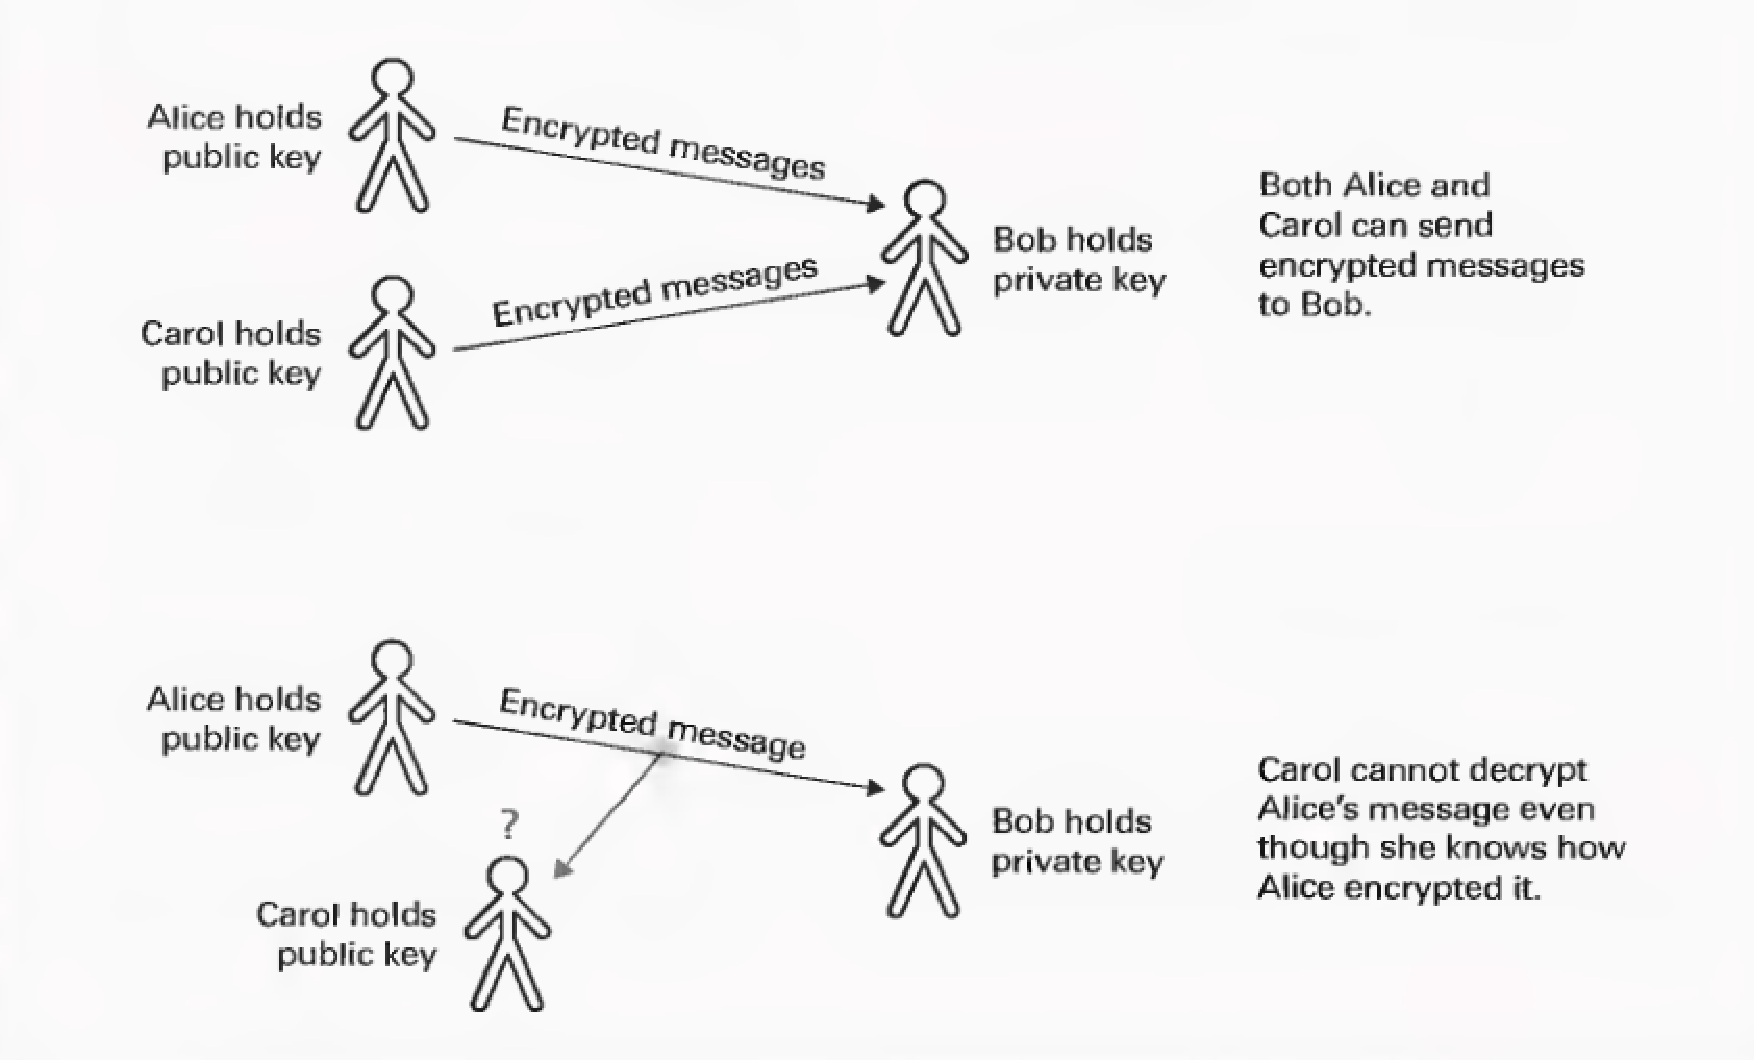
\includegraphics{ch5/fig416.pdf}}
  \caption{Mã khoá công khai}
  \label{fig:fig4.16}
\end{figure}

Tất nhiên, vẫn có những vấn đề không dễ phát hiện bị che dấu trong hệ thống mã hóa khóa
công khai. Một là phải đảm bảo rằng khóa công khai đang được sử dụng là khóa hợp pháp cho
người nhận thông điệp. Ví dụ, nếu bạn đang giao dịch với ngân hàng của bạn, bạn muốn chắc
chắn rằng khóa công khai mà bạn đang sử dụng để mã hóa là đúng của ngân hàng và nó không
bị mạo danh. Nếu một kẻ mạo danh tự giới thiệu là ngân hàng (một quá trình đã được giới
thiệu trước đó là spoofing) và đưa cho bạn khóa công khai của nó, các thông điệp mà bạn mã
hóa và gửi tới ``ngân hàng'' sẽ là có ý nghĩa đối với kẻ mạo danh chứ không phải cho ngân
hàng của bạn. Do đó, nhiệm vụ kết hợp các khóa công khai với các tổ chức uy tín là rất cần
thiết.

Một cách tiếp cận để có thể giải quyết được vấn đề này là thiết lập các điểm tin cậy trên
mạng Internet, thường được gọi là các \textbf{tổ chức chứng thực số} (CA: Certificate
Authority), nhiệm vụ của những tổ chức này là duy trì danh sách các đối tác cùng với các
khóa công khai của họ. Những tổ chức này, hoạt động dưới hình thức là các ứng dụng chủ,
sau đó cung cấp thông tin về khóa công khai tin cậy tới các ứng dụng khách thông qua các
gói được biết đến như là các chứng chỉ (certificates). Một \textbf{chứng chỉ số} là một
gói bao gồm tên của người tham gia và khóa công khai của anh ta hay cô ta. Ngày nay có rất
nhiều các tổ chức chứng thực số thương mại tồn tại trên mạng Internet, mặc dù nó cũng phổ
biến đối với các tổ chức nhằm duy trì chứng thực số của chính bản thân họ để bảo vệ sát sao việc điều khiển những hệ thống truyền thông vượt tầm kiểm soát của họ.

Cuối cùng, ta cũng nên bình luận về vai trò của những hệ thống mã hóa khóa công khai
trong việc giải quyết các vấn đề liên quan đến quá trình tạo sự \textbf{thẩm định quyền
  hạn} mà trên thực tế tác giả của một thông điệp cần gửi đi chính là người tham gia. Điểm
mấu chốt cần phê bình ở đây là trong những hệ thống mã hóa khóa công khai, vai trò của
khóa mã hóa và khóa giải mã có thể hoán đổi cho nhau. Thật vậy, văn bản có thể được mã hóa
bằng khóa bí mật, và khi chỉ có người tham gia vào hệ thống mới có quyền truy cập vào khóa
đó, bất kỳ văn bản nào được mã hóa đều phải bắt nguồn từ người tham gia đó. Theo cách này,
người giữ khóa bí mật có thể đưa ra một mẫu bít, gọi là chữ ký số, mà chỉ có người tham
gia hệ thống mới biết được cách thức sinh ra chữ ký số đó như thế nào. Bằng cách đính kèm
chữ ký số đó vào thông điệp, người gửi có thể chứng tỏ thông điệp cần gửi là đáng tin
cậy. Một chữ ký số có thể đơn giản như phiên bản mã hóa của chính thông điệp. Tất cả công
việc mà người gửi phải thực hiện là mã hóa thông điệp sẽ được truyền bằng cách sử dụng
khóa bí mật của anh ta hay cô ta (khóa mà được sử dụng để giải mã). Khi thông điệp được
nhận, người nhận sẽ dùng khóa công khai của người gửi để giải mã chữ ký số trong thông
điệp. Thông điệp đó đã thể hiện rõ là được đảm bảo đáng tin cậy bởi vì chỉ có người giữ khóa bí
mật mới có thể đưa ra được phiên bản mã hóa.

\subsection*{Những cách thức tiếp cận hợp pháp tới vấn đề an ninh mạng}
Một cách thức cho phép gia tăng sự an toàn của những hệ thống mạng máy tính là áp dụng các
biện pháp phòng chống mang tính pháp lý. Tuy nhiên, cũng có hai vấn đề trở ngại đối với
cách tiếp cận này. Trước tiên đó là việc tạo ra một hành động bất hợp pháp không ngăn chặn
được hành động đó. Tất cả những việc mà nó thực hiện là cung cấp một sự giúp đỡ hợp
pháp. Vấn đề trở ngại thứ hai là trạng thái nguyên thủy của các phương tiện hoạt động mạng
quốc tế thường rất khó khăn để có được sự giúp đỡ. Điều gì là bất hợp pháp đối với một
quốc gia có thể lại là hợp pháp đối với quốc gia khác. Cuối cùng thì việc gia tăng mức độ
an toàn của hệ thống mạng bằng các phương tiện pháp lý là một dự án quốc tế, và do đó cần
phải được thực hiện bởi những hội đồng hợp pháp--mà tổ chức có tiềm năng nhất là Tòa án
quốc tế (International Court of Justice) tại Hague.

Sau khi đã đưa ra những lời phủ nhận, ta cũng phải thừa nhận rằng, mặc dù chưa hoàn
hảo hơn, các lực lượng pháp lý cũng có một sự ảnh hưởng rất lớn, và do đó ta phải có
nhiệm vụ khám phá ra các bước hợp pháp mà đã đang được sử dụng để giải quyết các vấn đề
xung đột trong các hoạt động liên quan đến mạng máy tính. Với mục đích này, ta sử
dụng các ví dụ lấy ra từ các luật lệ liên bang của Hoa Kỳ. Những ví dụ tương tự có thể
được rút ra từ các cơ quan chính phủ của Liên minh Châu Âu.

Ta bắt đầu với sự gia tăng của phần mềm độc hại. Tại Hoa Kỳ, vấn đề này được chỉ ra
bởi luật Gian lận trong máy tính và Lạm dụng đạo luật (Computer Fraud and Abuse Act), mà
lần đầu tiên được thông qua năm 1984, mặc dù nó đã được sửa đổi nhiều lần. Đó là hành động
dưới này mà hầu hết các trường hợp liên quan đến việc giới thiệu về sâu và vi rút đã bị
truy tố. Tóm lại, các đạo luật đòi hỏi phải chứng minh rằng các bị đơn cố tình truyền tải
một chương trình hay dữ liệu có thể gây ra thiệt hại.


Đạo luật Gian lận trong máy tính và Lạm dụng đạo luật cũng bao gồm các trường hợp liên
quan đến sự hình thành hành vi trộm cắp. Đặc biệt, các hành động phạm pháp sẽ nhận được
bất cứ điều gì về giá trị thông qua việc truy cập trái phép vào một máy tính. Các phiên
toà có xu hướng chỉ định một mở rộng để làm sáng tổ cụm từ ``bất cứ điều gì về giá trị,''
và như vậy, đạo luật Gian lận trong máy tính và Lạm dụng Đạo luật đã được áp dụng nhiều
hơn cho các hành vi trộm cắp thông tin. Ví dụ, tòa án có quy định rằng các chỉ sử dụng một
máy tính có thể cấu thành nên ``bất cứ điều gì về giá trị.''

Sự đúng đắn của vấn đề riêng tư là ở chỗ khác, và có lẽ hầu hết đều gây ra các cuộc tranh
luận, các hoạt động mạng thường đối mặt với các vấn đề cơ sở pháp lý trong cộng đồng. Các
câu hỏi liên quan đến quyền giám sát những thông tin liên lạc từ phía các nhân viên của
một ông chủ và sự phản ảnh mức độ một nhà cung cấp dịch vụ Internet có thẩm quyền để truy
cập thông tin được truyền đạt bởi các khách hàng của nó đã tạo ra được số lượng đáng kể
những ý tưởng. Ở Hoa Kỳ, rất nhiều câu hỏi đã được đưa ra bởi Electronic Communication
Privacy Act (ECPA) vào năm 1986, có nguồn gốc của nó trong luật pháp để kiểm soát
wiretapping. Mặc dù các hành động kéo dài một cách nhàm chán, nhưng mục đích của nó có
được một vài trích dẫn ngắn ngủi. Đặc biệt, nó cũng nói rõ rằng

\begin{quotation} \small Trừ khi có những quy định cụ thể khác đã được đưa ra trong chương
  này, bất kỳ ai có ý chặn, cố gắng chặn, hay dẫn dắt người nào đó chặn hay cố gắng chặn
  bất kỳ một đoạn thư tín, một cuộc nói chuyện, hay một giao dịch điện tử… đều sẽ bị phạt
  theo quy định đã đề ra trong phần (4) hay sẽ bị giám sát nhu cầu theo quy định đề ra
  trong phần (5).
\end{quotation}
và
\begin{quotation} \small …bất kỳ cá nhân hay một tổ chức cung cấp dịch vụ truyền thông
  điện tử cho công chúng sẽ không được tiết lộ nội dung của bất kỳ một giao dịch truyền
  thông nào… mà dịch vụ đó được gửi tới bất kỳ ai hay một tổ chức nào đó chứ không chỉ đơn
  thuần là một cá nhân nhận thư hay nhận một giao dịch truyền thông như vậy hay một nhóm
  người nhận.
\end{quotation}


Tóm lại, ECPA xác định quyền giao tiếp của một cá nhân, đó là bất hợp pháp đối với một nhà
cung cấp dịch vụ Internet để phát hành các thông tin về sự truyền thông của các khách
hàng, và nó là bất hợp pháp cho nhân viên không có thẩm quyền nghe lén trái phép một cuộc
giao tiếp của người khác. Nhưng ECPA lại rời bỏ khỏi cuộc tranh luận. Ví dụ, các câu hỏi
liên quan đến các quyền của một chủ nhân để giám sát các giao tiếp của nhân viên sẽ trở
thành một vấn đề liên quan đến sự cấp phép, mà các toà án có xu hướng cấp quyền cho người
sử dụng lao động khi sự truyền thông được thực hiện bằng cách sử dụng các thiết bị của họ.


Hơn nữa, các hoạt động được tiếp tục trình lên một số cơ quan chính phủ có thẩm quyền để
giám sát sự truyền thông điện tử với một số hạn chế nhất định. Các điều khoản này đã trở
thành nguồn gốc của nhiều tranh cãi. Ví dụ, trong năm 2000, FBI tiết lộ sự tồn tại của hệ
thống, gọi là Carnivore, tiết lộ đó chỉ đưa ra các báo cáo về sự truyền thông của tất cả
các thuê bao thuộc một nhà cung cấp dịch vụ Internet hơn là một tòa án thiết kế nhắm mục
tiêu, và vào năm 2001 để phản ứng lại sự tấn công khủng bố trên Trung tâm Thương mại Thế
giới, hội Mỹ thông qua vấn đề USA PATRIOT (Liên minh Tăng cường Mỹ do cung cấp các Thích
hợp Công cụ bắt buộc để ngăn cản trở và khủng bố) Luật sửa đổi các hạn chế mà theo đó các
cơ quan chính phủ phải hoạt động.

\begin{figure}
  \begin{quotation}
    \noindent
    \textbf{Các đội phản ứng khẩn cấp máy tính}\vspace{0.3cm}
    \\
    Trong tháng 11 năm 1988, một sâu máy tính đã được thả vào Internet và đã gây ra sự sụp
    đổ một cách đáng kể các dịch vụ. Do đó, Cơ quan nghiên cứu các dự án cao cấp của Hoa
    Kỳ đã hình thành Đội phản ứng khẩn cấp máy tính CERT (CERT được đánh vần là ``SERT''),
    được đặt tại Trung tâm điều phối CERT tại trường Đại học Carnegie-Mellon. CERT chính
    là trung tâm quản lý sự an toàn của Internet (``watchdog''). Một trong số nhiệm vụ của
    trung tâm này là điều tra về các vấn đề an ninh, đưa ra các cảnh báo về an ninh, và
    thực hiện các chiến dịch nhận thức công cộng để cải thiện an ninh Internet. Trung tâm
    CERT duy trì một trang web có địa chỉ là \url{http://www.cert.org} mà tại đó đăng tải
    các bài viết, những thông báo về các hoạt động của nó.
  \end{quotation}
\end{figure}

%%% Local Variables: 
%%% mode: latex
%%% TeX-master: "../tindaicuong"
%%% End: 

\newpage
\section{Bài tập cuối chương}
\begin{multicols}{2}
  \begin{enumerate}

  \item Giao thức là gì? Chỉ ra 3 giao thức đã giới thiệu trong chương và mô tả mục đích
    của mỗi giao thức.

  \item Xác định và mô tả một giao thức máy trạm/máy chủ được sử dụng trong cuộc sống hàng ngày.

  \item Mô tả mô hình máy trạm/máy chủ.

  \item Chỉ ra 2 cách thức phân loại mạng máy tính.

  \item Sự khác nhau giữa hệ thống mạng mở và hệ thống mạng đóng?

  \item Có những giao thức dựa trên thẻ bài có thể được sử dụng để điều khiển quyền truyền
    phát tín hiệu mà không theo mô hình mạng vòng tròn. Thiết kế một giao thức dựa trên
    thẻ bài nhằm điều khiển quyền truyền phát tín hiệu trong một mạng LAN với mô hình mạng
    hình tuyến.

  \item Mô tả các bước thực hiện bởi một máy tính muốn truyền một thông điệp trong hệ
    thống mạng sử dụng giao thức CSMA/CD.

  \item Hub khác biệt so với Repeater như thế nào?

  \item Chỉ ra sự khác biệt khi so sánh Router với các thiết bị như Repeater, Bridge, Switch.

  \item Phân biệt một mạng nói chung với một mạng Internet nói riêng.

  \item Chỉ ra 2 giao thức điều khiển việc truyền tải một thông điệp trong một hệ thống mạng.

  \item 1.Mã hóa mỗi chuỗi bit sau đây bằng cách sử dụng ký hiệu dấu chấm thập phân:
    \begin{enumerate}
    \item $000000010000001000000011$

    \item $1000000000000000$

    \item $0001100000001100$
    \end{enumerate}

  \item Chuỗi bit tương ứng với mỗi mẫu ký hiệu dấu thập phân sau:
    \begin{enumerate}
    \item $0.0$ 
    \item $25.18.1$
    \item $5.12.13.10$
    \end{enumerate}

  \item Giả sử địa chỉ của một máy chủ trên mạng Internet là $138.48.4.123$. Địa chỉ tương
    ứng ở dạng Hexa (hệ cơ số mười sáu) là gì?

  \item Nếu phần xác định địa chỉ mạng của một vùng là $192.207.77$, có bao nhiêu địa chỉ
    IP có thể sử dụng được để cấu hình cho các máy tính trong vùng? (Sau khi bạn tìm ra
    được câu trả lời, bạn có thể phỏng đoán rằng có thể có ít hơn địa chỉ IP so với số
    lượng máy tính có trong vùng, và đây cũng là trường hợp thường xảy ra. Một giải pháp
    để có thể đặt địa chỉ IP cho các máy tính chỉ khi máy cần dùng đến, đó là hệ thống đặt
    địa chỉ IP động).


  \item Nếu một địa chỉ theo dạng tên dễ nhớ của một máy tính trên mạng Internet có dạng:\\
    \url{batman.batcave.metropolis.gov}\\ Bạn có thể phỏng đoán vùng chứa máy tính đó là
    gì?


  \item Giải thích các thành phần xuất hiện trong địa chỉ\\ \url{kermit@animals.com}

  \item Trong trường hợp truyền tải tệp sử dụng giao thức FTP, sự khác biệt rõ nét giữa
    ``tệp văn bản'' và ``tệp nhị phân'' là gì?

  \item Vai trò của máy chủ thư trong một vùng là gì?

  \item Định nghĩa lại mỗi khái niệm sau:
    \begin{enumerate}
    \item Name server
    \item Domain
    \item Router
    \item Host
    \end{enumerate}

  \item Vai trò của Network Virtual Terminal trong giao thức telnet?

  \item Định nghĩa lại mỗi khái niệm sau:
    \begin{enumerate}
    \item Hypertext
    \item HTML
    \item Browser
    \end{enumerate}


  \item Có nhiều cách nhìn nhận về sự hoán đổi giữa hai thuật ngữ \textit{Internet} và
    \textit{World Wide Web} trong mạng Internet. Mỗi thuật ngữ trên đề cập tới vấn đề gì?

  \item Khi thực hiện xem một trang web đơn giản, yêu cầu trình duyệt hiển thị nguồn của
    trang web đó. Sau đó xác định cấu trúc cơ bản của tài liệu nguồn hiện ra, xác định
    phần tiêu đề và phần thân của tài liệu đồng thời chỉ ra một vài câu lệnh tìm thấy
    trong mỗi phần.


  \item Sửa tài liệu HTML duới đây với yêu cầu là từ ``Rover'' được liên kết tới tài liệu
    khác theo đường dẫn sau: \url{http://animals.org/pets/dogs.html}
\begin{verbatim}
<html>
<head>
<title>Example</title>
</head>
<body>
<h1>My Pet Dog</h1>
<p>My dog’s name is Rover./p>
</body
<html>
\end{verbatim}

  \item Vẽ ra một bản phác họa mô tả xem một tài liệu HTML sau đây sẽ xuất hiện như thế
    nào khi nó hiển lên màn hình máy tính.
\begin{verbatim}
<html>
<head>
<title>Example</title>
</head>
<body>
<h1>My Pet Dog</h1>
<p>My dog’s name is Rover./p>
</body
<html>
\end{verbatim}

  \item Xác định các phần tử cấu thành trong địa chỉ sau và nêu ý nghĩa của chúng:\\
    \url{http://lifeforms.com/animals/moviestars/kermit.html}

  \item Xác định các phần tử cấu thành trong các địa chỉ vắn tắt sau:

    \begin{enumerate}
    \item \url{http://www.farmtools.org/windmills.html} 

    \item \url{http://castles.org/} 

    \item \url{www.coolstuff.com}
    \end{enumerate}

  \item Trình duyệt sẽ đáp ứng lại khác nhau như thế nào khi bạn yêu cầu nó tìm một tài
    liệu qua địa chỉ:\\
    \url{telnet://stargazer.universe.org} \\
    so với \\
    \url{http://stargazer.universe.org }

  \item Đưa ra $2$ ví dụ về các hoạt động ở phía máy trạm và $2$ ví dụ về các hoạt động ở
    phía máy chủ.

  \item Giả sử mỗi máy tính trong một mạng vòng tròn được lập trình để truyền tức thì về
    cả hai phía các thông điệp mà xuất phát từ một máy trạm nào đó và được đánh địa chỉ
    gửi tới tất cả các trạm làm việc khác trong mạng. Hơn nữa, giả sử điều này được thực
    hiện thông qua việc giành được quyền truy cập đầu tiên tới đường truyền truy cập tới
    các máy phía bên trái, duy trì truy cập này cho tới khi đường truyền truy cập phía bên
    phải được yêu cầu và sau đó truyền tải thông điệp đi. Xác định khi nào
    \textup{deadlock} (xem thêm Mục~\ref{sec:3.4}) xảy ra nếu tất cả các máy tính trong
    mạng đều cố gắng gửi một thông điệp cùng tại một thời điểm.


  \item Mô hình tham chiếu OSI là gì?

  \item Trong một hệ thống mạng được thiết kế theo dạng hình tuyến, trục bus là một dạng
    tài nguyên không thể chia sẻ được mà trong đó các máy trạm đều cần phải cạnh tranh với
    nhau để có thể gửi được các thông điệp một cách có thứ tự. Trong trường hợp này, tắc
    nghẽn (deadlock) (xem thêm Mục~\ref{sec:3.4}) được điều khiển như thế nào?

  \item Liệt kê 4 tầng trong mô hình Internet và xác định nhiệm vụ được thực hiện bởi mỗi
    tầng.

  \item Tại sao tầng vận chuyển lại thực hiện chia nhỏ các thông điệp (messages) lớn thành
    những gói tin nhỏ (packets).

  \item Khi một ứng dụng yêu cầu tầng vận chuyển sử dụng giao thức TCP để truyền tải một
    thông điệp, những thông điệp nào khác sẽ được truyền tải bởi tầng này nhằm đáp ứng đủ
    các yêu cầu của tầng ứng dụng?

  \item Theo cách thức nào mà có thể nhận xét giao thức TCP được xem là tốt hơn so với
    giao thức UDP trong việc thực thi tại tầng vận chuyển? Trong trường hợp nào thì giao
    thức UDP được coi là tốt hơn so với giao thức TCP?

  \item Điều gì khẳng định nhận xét UDP là một giao thức không có kết nối
    (connectionless)?

  \item Tại tầng nào trong mô hình phân cấp giao thức TCP/IP ta có thể đặt một bức tường
    tại đó nhằm lọc các luồng giao thông đi tới theo:
    \begin{enumerate}
    \item Nội dung của thông điệp

    \item Địa chỉ nguồn của thông điệp

    \item Kiểu của ứng dụng
    \end{enumerate}

  \item Giả sử bạn muốn thiết lập một bức tường lửa nhằm lọc các thông điệp thư điện tử
    chứa các câu hay cụm từ chỉ định. Bức tường lửa này nên được đặt tại cổng vào ra của
    vùng hay đặt tại máy chủ thư của vùng? Giải thích câu trả lời của bạn.

  \item Máy chủ proxy là gì và lợi ích của nó đem lại?

  \item Tóm tắt các nguyên lý của mật mã hóa khóa công khai.

  \item Mạng toàn cầu Internet thường gây nguy hại cho một máy tính không được bảo vệ theo
    cách thức nào?

  \end{enumerate}
\end{multicols}

%%% Local Variables: 
%%% mode: latex
%%% TeX-master: "../tindaicuong"
%%% End: 


%%% Local Variables: 
%%% mode: latex
%%% TeX-master: "../tindaicuong"
%%% End: 
